\documentclass[degree=bachelor,tocarialchapter]{thuthesis}
% 选项
%   degree=[bachelor|master|doctor|postdoctor], % 必选,学位类型
%   language=[chinese|english], % 可选(默认:chinese),论文的主要语言
%   secret,                % 可选(默认:关闭),是否有密级
%   tocarialchapter,       % 可选(默认:关闭),章目录中使用黑体(这项表示同时打开下面两项)
%   tocarialchapterentry,  % 可选(默认:关闭),单独控制章标题在目录中使用黑体
%   tocarialchapterpage,   % 可选(默认:关闭),单独控制章页码在目录中使用黑体

% 所有其它可能用到的包都统一放到这里了,可以根据自己的实际添加或者删除。
\usepackage{thuthesis}
\usepackage{xcolor}
\renewcommand{\emph}[1]{\textcolor{purple}{\textit{#1}}} % for emph color

\usepackage{siunitx} % \SI{1.234}{\m\per\square\s} \SI{1e-4}{\metre}
\DeclareSIUnit{\rad}{rad} % \rad is removed frmo siunitx 2 since it is not a SI unit. 

% \usepackage{amsmath}
\newcommand\vect{\mathbf}
% \newcommand\matr{\mathbf} % \matrix is defined in LaTeX2e kernel
% \newcommand\tens{\mathcal}

\usepackage{romannum}  % \Romannum{3} \romannum{3}


\def\degree{${}^{\circ}$} % degree symbols
\sisetup{math-micro=\text{µ},text-micro=µ} 
% Very strange that the micro symbol does not appear in \SI{}{}, 
% this is a bug found at https://tex.stackexchange.com/questions/33965/siunitx-µ-doesnt-work 
\usepackage[super]{nth} % 1st, 2nd, ...


% Conflict with thuthesis
% \usepackage[math-style=ISO]{unicode-math} % XeTeX driver only supports unicode.  (hyperref)  Enabling option `unicode'. 
% Sometimes pasted texts may contain unicode math symbols which may cause compiling errors, the package is capable to help you skip those trivial errors caused by compiling those symbols which used to be uncompilable properly.

\usepackage{etoolbox}
\newbool{isBeamer} 
% \booltrue{isBeamer}
\boolfalse{isBeamer}
% \ifbool{isBeamer}{<true>}{<false>}

\usepackage{booktabs}

\makeatletter
\newcommand{\rmnum}[1]{\romannumeral #1}
\newcommand{\Rmnum}[1]{\expandafter\@slowromancap\romannumeral #1@}
\makeatother
\usepackage{hyperref}


% \usepackage[T1]{fontenc} //This may cause some alignment problem in cover
\usepackage[utf8]{inputenc}


% Special scientist naem 
\usepackage{xspace}
\newcommand{\Poincare}{Poincar\'e\xspace}
\newcommand{\adele}{ad\`ele\xspace}
\newcommand{\Cech}{\v{C}ech\xspace}
\newcommand{\Erdos}{Erd\H{o}s\xspace}
\makeatletter
\newcommand{\etale}{\'etal\@ifstar{\'e}{e\xspace}}
\makeatother


\newcommand{\vE}{\vect{E}}
\newcommand{\vx}{\vect{x}}
\newcommand{\vv}{\vect{v}}
\newcommand{\ftxv}{f(t, \vect{x}, \vect{v})}
\newcommand{\bbRRR}{\bbR^{3}}
\newcommand{\bbRx}{\bbR_{x}^{3}}
\newcommand{\bbRv}{\bbR_{v}^{3}}

% 定义所有的图片文件在 figures 子目录下
\graphicspath{{figures/}}



% 可以在这里修改配置文件中的定义。导言区可以使用中文。
% \def\myname{薛瑞尼}

\begin{document}

%%% 封面部分
\frontmatter
\thusetup{
  %******************************
  % 注意:
  %   1. 配置里面不要出现空行
  %   2. 不需要的配置信息可以删除
  %******************************
  %
  %=====
  % 秘级
  %=====
  % secretlevel={秘密},
  % secretyear={10},
  %
  %=========
  % 中文信息
  %=========
  ctitle={三维扰动场对等离子体边界磁拓扑影响的协同优化模拟},
  cdegree={工学本科},
  cdepartment={工程物理系},
  cmajor={工程物理},
  cauthor={魏文崟},
  csupervisor={梁云峰教授},
  cassosupervisor={高喆教授}, % 副指导老师
  ccosupervisor={高喆教授}, % 联合指导老师
  % 日期自动使用当前时间,若需指定按如下方式修改:
  % cdate={超新星纪元},
  %
  % 博士后专有部分
  % catalognumber     = {},  % 可以留空
  % udc               = {},  % 可以留空
  % id                = {},  % 可以留空: id={},
  % cfirstdiscipline  = {},  % 流动站(一级学科)名称
  % cseconddiscipline = {},  % 专 业(二级学科)名称
  % postdoctordate    = {},  % 工作完成日期
  % postdocstartdate  = {},  % 研究工作起始时间
  % postdocenddate    = {},  % 研究工作期满时间
  %
  %=========
  % 英文信息
  %=========
  etitle={Collaborative Optimization of Multiple 3D Magnetic Perturbation Fields according to Their Effects on Plasma Edge Magnetic Topology in EAST tokamak},
  % 这块比较复杂,需要分情况讨论:
  % 1. 学术型硕士
  %    edegree:必须为Master of Arts或Master of Science(注意大小写)
  %             “哲学、文学、历史学、法学、教育学、艺术学门类,公共管理学科
  %              填写Master of Arts,其它填写Master of Science”
  %    emajor:“获得一级学科授权的学科填写一级学科名称,其它填写二级学科名称”
  % 2. 专业型硕士
  %    edegree:“填写专业学位英文名称全称”
  %    emajor:“工程硕士填写工程领域,其它专业学位不填写此项”
  % 3. 学术型博士
  %    edegree:Doctor of Philosophy(注意大小写)
  %    emajor:“获得一级学科授权的学科填写一级学科名称,其它填写二级学科名称”
  % 4. 专业型博士
  %    edegree:“填写专业学位英文名称全称”
  %    emajor:不填写此项
  edegree={Bachelor of Engineering Physics},
  emajor={Engineering Physics},
  eauthor={Wei, Wenyin},
  esupervisor={Professor Liang, Yunfeng},
  % eassosupervisor={Chen Wenguang},
  % 日期自动生成,若需指定按如下方式修改:
  % edate={December, 2005},
  %
  % 关键词用“英文逗号”分割
  ckeywords={扰动场, 边界局域模, 共振磁扰动, 高 m 线圈, 低杂波, 螺旋电流丝},
  ekeywords={magnetic perturbation field, edge localized mode (ELM), resonant magnetic perturbation (RMP),high m coil, lower-hybrid (LH), helical current filament (HCL)}
}

% 定义中英文摘要和关键字
\begin{cabstract}
  本课题来自目前的先进托卡马克位型所面临的现实问题,尽管参数优良的 \Hmode 等离子体使得聚变达到所需参数目标有了更大的可能性,但同时也带来了新的问题。\Hmode 下等离子体边界高压力梯度和强电流密度蕴含的自由能,引起了边界局域模不稳定性。边界局域模会引起热负荷和粒子流强出现近似周期性的脉冲峰值,而这在 DEMO 堆中是不被允许的。

  为了抑制边界局域模, EAST 上先后测试了共振磁扰动线圈 RMP、高 m 线圈和低杂波驱动的螺旋电流丝,这三种扰动场产生机制有所差异,产生的效果也不尽相同。为了使扰动场相互配合达到最优的弱化乃至抑制边界局域模的效果,对它们在等离子体边界造成的扰动场协同作用的研究是很有必要的。 (1) 低 n 线圈,一般称为 RMP 线圈,布置在腔内,它激发起环向模数为 $n=1,2$ 的扰动场在 \east, \ddd 等托卡马克装置上验证了其抑制边界局域模的效应。 (2) 高 m 线圈,是 EAST 团队近两年实验中的线圈,在等离子体环外加上一组四个的线圈,它的特征是扰动场环向模数 $n$ 分布较宽,极向模数 $m$ 较高,由于一组高 $m$ 线圈只分布在一个极向截面处,扰动场的局域性很强。(3) 低杂波驱动的螺旋电流丝,电流丝的具体物理机制还不甚明晰,但其亦能调节边界磁拓扑。由于低杂波天线不像共振磁扰动线圈在腔内易受到损坏且激发出的螺旋电流丝紧靠边界,它有望在 DEMO 堆及日后商业堆中灵活地调节磁拓扑结构。
  
  第二章便进入本文主体,线圈之间如何配合以能够对等离子体施加合适的磁扰动场,为此对磁扰动场径向分量在边界附近的磁面 Fourier 分析得到的磁谱 $\tilde{b}^1_{mn}$ 和 \Poincare 图是必要的。这一章的主体是通过扰动场之间的配合达到较好的抑制 ELM 及保持芯部等离子体较好约束的效果。进一步在第三章中将讨论不同扰动场的配置下第一壁材料上的热负荷和粒子流分布。尽管主要依赖于对 ELM 的抑制效果来选择磁扰动场,但基于扰动场的热负荷优化分布或时间调制能够给出了一种新的调节视角。%对下一代托卡马克而言,%\Hmode 等离子体会造成难以承受的热流和粒子流,
  % 扰动场可以此提供一种调节手段,避免脉冲式的 ELM 破裂造成的材料损害。

\end{cabstract}

% 如果习惯关键字跟在摘要文字后面,可以用直接命令来设置,如下:
% \ckeywords{\TeX, \LaTeX, CJK, 模板, 论文}

\begin{eabstract}
  The thesis discusses the realistic problem confronted by advanced tokamaks research. Though better confinement is obtained with \Hmode plasma than \Lmode, which makes it possible to achieve the threshold acquired by the fusion energy, new problems are also coming. The free energy stored in the high pressure gradient and strong current density in the edge of confined plasma induces edge localized mode (ELM) instability. ELM may cause too intense transient pulses of heat load and particle flux to sustain, which is not allowable in future tokamaks.

  In order to realize ELM suppression, multiple varieties of perturbation fields have been tested in EAST, \textit{i.e.} resonant magnetic perturbation coils, high $m$ coils and helical current filaments induced by lower hybrid wave. Each of these approaches has advantages and disadvantages. It is necessary to research on the collaborative effect if an optimal ELM suppression effect is anticipated. (1) Low n coils,also known as RMP coils, are distributed inside the vessel to stimulate the perturbant field with dominant toroidal mode number $n=1,2$. Its effect to mitigate or suppress ELM is verified in \east, \ddd tokamaks \textit{etc.}. (2) High m coils are under design by \east team in these two years. Normally four coils are imposed in one poloidal crosssection $\phi=\text{const.}$ with various theta. High $m$ coils have the characteristics that perturbant spectrum distribute widely in toroidal mode number $n$ while relatively high in poloidal mode number $m$. (3)Helical current filanments(HCFs) induced by lower hybrid waves(LHW). LHW is originally designed to drive core plasma current by Landau damping, but experimental evidence shows that there exists helical current filaments in the scrape-off layer (SOF) while LHW system switches on. Because of the fact that LHW antennas are shielded by limiters, therefore not easy to be damaged, and HCFs are close to the plasma edge, it has the potential to modify the magnetic topology near the edge of plasma flexibly in DEMO and next-generation tokamaks.

  Appropriate collaborative coils setup are discussed in chapter two to exert the suitable perturbation field on the plasma, in which the Fourier spectrum $\tilde{b}^1_{mn}$ of the radial component of perturbation field near the edge of plasma and \Poincare plots are necessary to analyze the topology. How to acquire a satisfactory perturbant result, \textit{i.e.} suppress ELM and sustain well confinement of plasma, constitutes the main content of chapter two. Furthermore, the heat load distribution patterns of various perturbant field combinations are analyzed in chapter three. Though we mainly rely on the ELM suppression effect to alter perturbant recipes, the possibility of adjustment of heat load distribution is considered to provide another perspective on the perturbant field. For next generation tokamaks, \Hmode plasma causes unafforable heat flux and particle flux pulses to the plasms-facing components, for which schemes to adjust the heat pattern are required.
\end{eabstract}

% \ekeywords{\TeX, \LaTeX, CJK, template, thesis}

% 如果使用授权说明扫描页,将可选参数中指定为扫描得到的 PDF 文件名,例如:
% \makecover[scan-auth.pdf]
\makecover

%% 目录
\tableofcontents

%% 符号对照表
\begin{denotation}[3cm]
\item[$(R, \phi, Z)$] 磁约束聚变常用柱坐标
\item[$\kappa$] 热导率或者等离子体延伸率,视其上下文而定。
\item[$q, \vect{q}, |\vect{q}|$] $\vect{q}$ 表示热流强度,$|\vect{q}|$ 表其幅值,$q$ 本文中均表示安全系数
\item[$\delta$] 三角变形系数 triangularity
\item[$a, R_0$] 托卡马克装置小半径、大半径  
\item[$\varepsilon$] 环径比 $=a/R_0$ aspect ratio 
\item[ELM] 边界局域模 Edge Localized Mode
\item[RMP] 共振扰动场线圈 Resonant Magnetic Perturbance
\item[ICRH] 离子回旋共振加热 Ion Cyclotron Resonance Heating  
\item[ITER] 国际热核聚变实验堆计划 International Thermonuclear Experimental Reactor 
\item[DEMO] 示范聚变堆 DEMOnstration power plant
\item[SOL] 刮削层 scrape-off layer
\item[HRB] 螺旋辐射带 Helical Radiation Belt  
\item[HCF] 螺旋电流丝 Helical Current Filament
\end{denotation}



% % 也可以使用 nomencl 宏包:

% \printnomenclature[3cm]




%%% 正文部分
\mainmatter
\chapter{课题介绍}

\section{EAST}
EAST (\textbf{E}xperimental \textbf{A}dvanced \textbf{S}uperconducting \textbf{T}okamak) 实验先进超导托卡马克位于合肥等离子体物理研究所。

\begin{table}[htb]
    \centering
    \caption{\east 设计参数}
    \label{tab:east_parameter}
    \begin{tabularx}{\linewidth}{lXlXlX}
        \toprule[1.5pt]
        $R$ 大半径 &   & $a$ 小半径 &  & $\delta$ 三角形变系数 & \\
        $B_t$ 环向中心磁感应强度 &   & *** &  & *** & \\
        % \midrule[1pt]
        \bottomrule[1.5pt]
    \end{tabularx}
\end{table}

\section{边界局域模}
边界局域模 (Edge Localize Mode, ELM) 是一种在\Hmode 等离子体中存在的磁流体不稳定性,相比于\Lmode 等离子体,\Hmode 等离子体边界密度梯度和温度梯度更为显著,当梯度达到阈值时,等离子体边界会间歇性地将能量和粒子从边界脉冲式地释放出去,周而复始。\Hmode 最早在ASDEX 托卡马克上被发现了,其特点在于边界压强梯度较大,从而形成台基区(pedestal)。ELM 在 \ddd 上得到了充分的研究,其分类很大程度上受到了 \ddd 的影响,其提出的 。不过 ELM 并不是完全不好,重复可控的边界局域模发生也可以帮助控制等离子体中的粒子存量。



边界局域模相关的理论难以给出能量和粒子损失速率的定量描述,于是便很难和实验的对比。可以比较的是实验观测到的时间尺度,例如,边界局域模的上升时间尺度,持续时间尺度以及在以及边界局域模重复频率的变化趋势,另外,边界局域模发生的径向范围可以用理论给出,而且可以和实验的发现进行一个对比。

从目前聚变等离子体中 ELM 现象来看,\cite{zohm_edge_1996} 将其清晰地划分为三种。


\begin{itemize}
    \item \textit{\typeone ELM}  重复频率 $\nu_{ELM}$ 随着加热功率的增加而增加。在高温时,\typethr 的 ELM 已经被抑制住了,此时理想气球模限制了可以达到的边界最大压力梯度 $\alpha/\alpha_{\text{crit}}\approx 1$,如果理想气球模耦合了一种低 $n$ 的不稳定性(由于强边界电流密度,很有可能是一种类扭结的不稳定性),\typethr ELM 就会发展起来。如果通过等离子体塑形可以使等离子体边界符合气球模的第二类稳定域,那么该类型 ELM 就会被抑制住,而此时对边界压力梯度的限制,就将由低 $n$ 的磁流体不稳定性所决定。\\
    ELM 在目前的实践中,没有显著的磁前兆振荡被检测到,不过这类 ELM 发生之前会有密度湍流波动的增强。这类不稳定性会使得 $D_\alpha$ 信号产生间断的剧烈爆发。
    \item \textit{\typethr ELM} 重复频率 $\nu_{ELM}$ 随着加热功率的增加而减小.在 L-H 转换之后,在边界的电子温度不太高的情况下,由于边界输运壁垒的存在,边界的压力梯度和电流密度变得更加强烈,构成了有阻磁流体不稳定性的自由能的源头。但随着输入功率增高,足够高的温度使阻尼效应可忽略时,\typethr ELM 会被抑制住。\\
    可以通过赤道面的磁探针获得其前兆磁湍动,频率范围 $\nu_{\text{prec}}\approx \SI{50}{\kilo\hertz} \sim \SI{70}{\kilo\hertz}$ 。等离子体边界压力梯度显著低于理想气球模的极限,即 $0.3\leq \alpha/\alpha_{\text{crit}}\leq 0.5$。
    \item \textit{Dithering Cycles, 振荡循环型} 在 L-H 转换过程中,由于\Hmode 功率的滞后而在阈值上下而往复的循环是有可能的。边界的压力和电流梯度和 \Lmode 时类似,所以可以说,振荡周期型不是一种典型的磁流体不稳定性,而是一种 L-H-L 模转换连续发生的现象。
\end{itemize}

尽管受 ELM 复杂的非线性物理所限,这样的物理描述不能作为一种 ELM 的精确定义。但这种唯象的理解是基于实验观测到的结果,并且和目前对磁流体稳定性的分析相差不甚。



\cite{2003PPCF...45.1549L} 基于目前装置上实验参数的外推结果,\iter 上 \typeone ELM 可能会导致损失 $5\sim \SI{22}{\mega\joule}$ ,其中约一半分布在 $\sim \SI{1}{\meter^2}$ 壁上的热沉积范围\inlinecite{Loarte_2014}。壁材料瞬态接受的能量密度在 $2.5\sim \SI{11}{\mega\joule/\meter^2}$,是目前材料(钨或碳纤维材料)承受热负荷能力的 $5\sim 20$ 倍。如何控制或者抑制 ELMs 成为了相当关键的一个问题。由共振磁扰动(RMP)引起的共振及边界随机场被认为可以抑制在等离子体边界周期性或拟周期性的破裂。


不过等离子体对扰动的响应往往会屏蔽掉 RMP 线圈施加的影响并且大大地降低磁场的随机程度\inlinecite{sun_nonlinear_2016},这使得通过 RMP 线圈有效可靠地抑制边界局域模 ELM 需要深入的研究。

目前学界对 ELM 的弱化和抑制之间的关键区别还不明晰,同时等离子体对 ELM 抑制的线性/非线性响应均有待探索。

\section{本课题中涉及的扰动场}

在聚变等离子体中用到的外加扰动场(magnetic perturbation, MP)是指螺旋形或鞍形线圈产生的量级为 $\delta B_r/\delta B_t=10^{-5}\sim 10^{-3}$ 的磁场扰动。将外加磁扰动在磁面坐标系中并进行空间傅里叶分解运算,可以得到多个极向模数为 $m$, 环向模数为 $n$ 的分量。其分布在 $q_{min}<m/n<q_a$ 分量螺旋程度与安全因子为 $q_s=m/n$ 的有理面相同的螺旋度,从而可以实现通过共振效应对有理面上的不稳定性造成较大影响。因此,磁扰动中的这些分量特别地命名为共振磁扰动(Resonant Magnetic Perturbation, RMP)。RMP 使得其在某个特定的磁面产生共振(通常指等离子体边界区域)。这里共振指的是在目标磁面施加的径向磁场螺旋度和平衡场的相近。

RMP 的目的在于稳定 ELM,避免脉冲式的粒子流和热负荷,使得直面等离子体的材料能够长时间工作。


\subsection{腔内低场侧 RMP}
一套 RMP 线圈系统于 2014 年安装在 EAST 的低场侧,它包含有两组线圈($2*8=16$)。EAST 团队通过扰动场环向模数为 $n=1, 2$ 的 RMPs 实现了 \typeone 边界局域模的弱化和完全的抑制。

\subsection{高 m 线圈}
等离子体所新近研发的高 m 线圈 \inlinecite{zhang_highm} 激发出的扰动场有着高 m,宽 n 特征,分为上下对称两组($2*2=4$),几何最大电流为 \SI{5}{\kilo\ampere}。 
物理计算过程中采用的线圈几何尺寸如图 \ref{fig:highm-pos} 所示。其对等离子体的影响现正被研究,由于高 $m$ 线圈组设计位于一个极向截面内,即 $\phi\equiv \text{const}$ 处,其对等离子体的影响局域性很明显,此类强局域性扰动磁场对等离子体边界稳定性的影响也可以从中得到研究。

采用与现有 RMP 系统相同线圈材料 线圈位置位于低场侧限制器后方,利用限制器作为线圈的保护,尽可能靠近等离子体 


\begin{figure}[htbp]
    \centering%
    % \hspace{4em}%
    \begin{subfigure}{0.45\textwidth}
      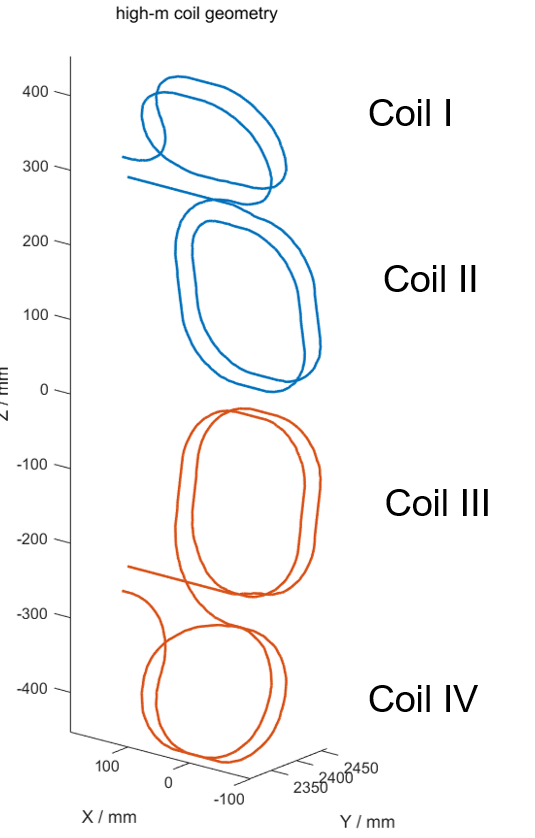
\includegraphics[height=8cm]{highm/coil_geometry.png}
      \caption{高 $m$ 线圈的立体几何位置}
    \end{subfigure}
    % \hspace{4em}%
    \begin{subfigure}{0.45\textwidth}
      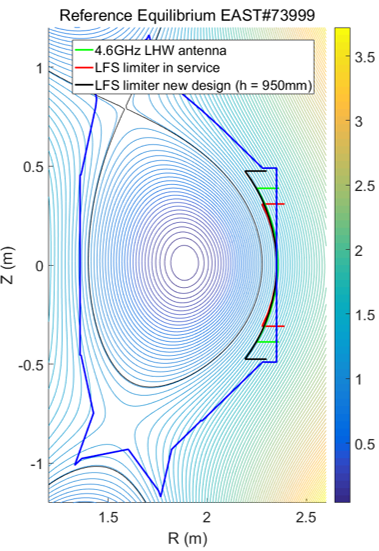
\includegraphics[height=8cm]{highm/coil_limiter_pos.png}
      \caption{极向截面上高 $m$ 线圈的位置}
    \end{subfigure}
    \caption{高 $m$ 线圈在 \east 中的设计和所处的几何位置,来源于张华祥研究员 \cite{zhang_highm} 的报告}
    \label{fig:highm-pos}
  \end{figure}

根据两组线圈内电流的相对方向,有两种工作模式,见图 \ref{fig:highm-pos}。\textit{主要工作模式}时两组线圈通同向电流;\textit{次要工作模式}时则反向。



\begin{figure}[htbp]
    \centering%
    \begin{subfigure}{0.33\textwidth}
      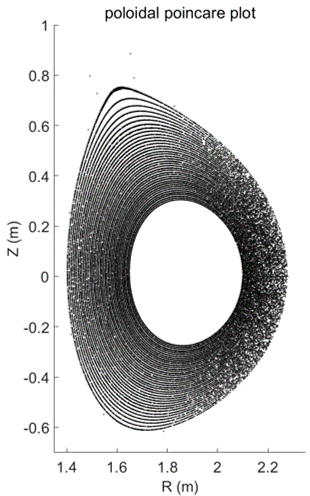
\includegraphics[height=8cm]{highm/original_equilibrium_no_high_m.png}
      \caption{平衡场}
    \end{subfigure}%
    % \hspace{4em}%
    \begin{subfigure}{0.33\textwidth}
      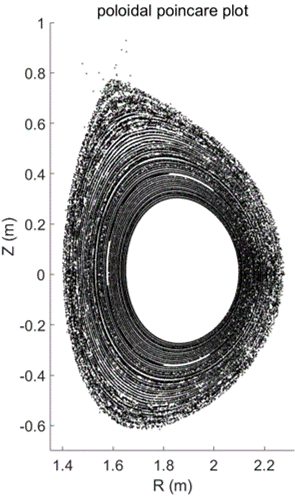
\includegraphics[height=8cm]{highm/original_equilibrium_with_high_m.png}
      \caption{主要工作模式的线圈场}
    \end{subfigure}
    % \hspace{4em}%
    \begin{subfigure}{0.33\textwidth}
      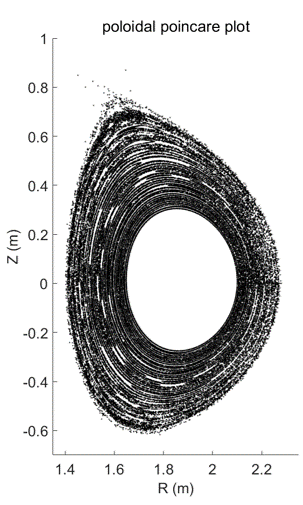
\includegraphics[height=8cm]{highm/original_equilibrium_with_high_m_inverse.png}
      \caption{次要工作模式的线圈场}
    \end{subfigure}
    \caption{高 m 线圈作用下的平衡场扰动情况,次要工作模式下的磁扰动情况较主要模式更深,来源于张华祥研究员 \cite{zhang_highm} 的报告}
    \label{fig:highm-three-subfig-poincare}
  \end{figure}

  
\begin{figure}[htbp]
    \centering%
    % \hspace{4em}%
    \begin{subfigure}{0.8\textwidth}
        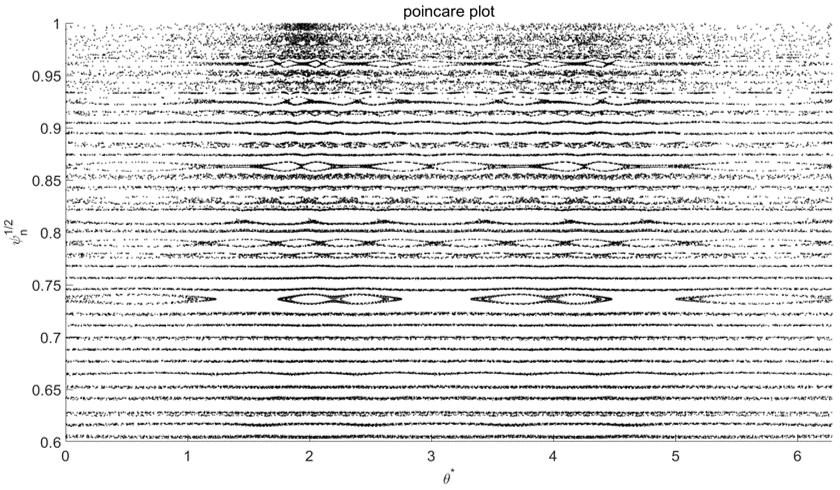
\includegraphics[height=6.6cm]{highm/stretched_poincare_primary_state.png}
        \caption{高 $m$ 线圈主要工作模式下展开的 \Poincare 图}
    \end{subfigure}
    % \hspace{4em}%
    \begin{subfigure}{0.8\textwidth}
        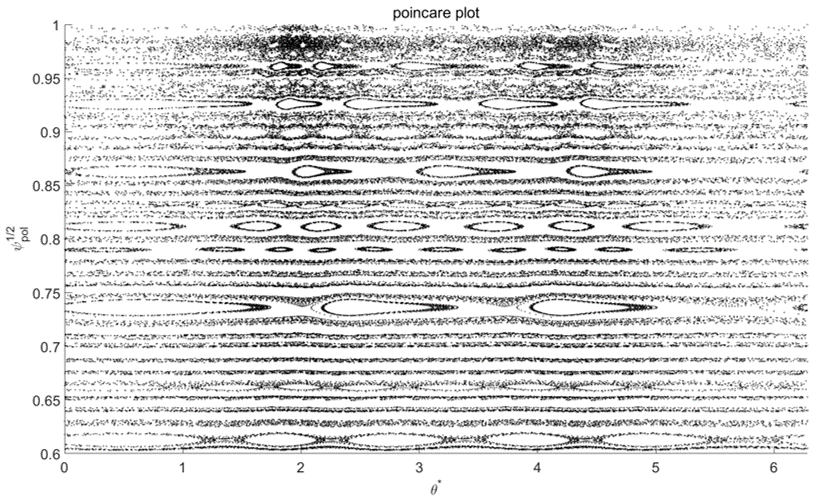
\includegraphics[height=6.6cm]{highm/stretched_poincare_secondary_state.png}
        \caption{高 $m$ 线圈次要工作模式下展开的 \Poincare 图}
    \end{subfigure}
    \caption{高 $m$ 线圈作用下的 \Poincare 图,次要工作模式下的磁扰动情况较主要模式更深,来源于张华祥研究员 \cite{zhang_highm} 的报告}
    \label{fig:highm-stretched-poincare}
\end{figure}
  

% \begin{figure}[H] % use float package if you want it here
%     \centering
%     \includegraphics{thu-whole-logo.pdf}
%     \caption{利用 Xfig 制图}
%     \label{fig:xfig1}
% \end{figure}







\subsection{低杂波驱动的螺旋电流丝}
RMP 其致命的弱点是线圈置于腔内,这在 DEMO 堆的设计中是不被允许的,研究人员只能通过其他手段来改变边界磁拓扑。 在低杂波加热设计之外得到的螺旋电流丝,是一个很有吸引力的在下一代聚变设备中应用的 RMP 手段。

低杂波加热原本用于芯部等离子体电流驱动,它通过朗道阻尼将动量传给等离子体,可以实现不依赖于离子回旋共振加热 (ICRH) 的长脉冲\Hmode 运行。但在原本被设计好的加热作用之外,还在 \ddd、\east 等不同装置上发现了低杂波驱动的螺旋电流丝,低杂波启动后毫秒内电流丝即响应出现,电流丝数量和托卡马克中低杂波天线的行数相同。


\begin{figure}[htbp]
    \centering%
    % \hspace{4em}%
    \begin{subfigure}{0.45\textwidth}
        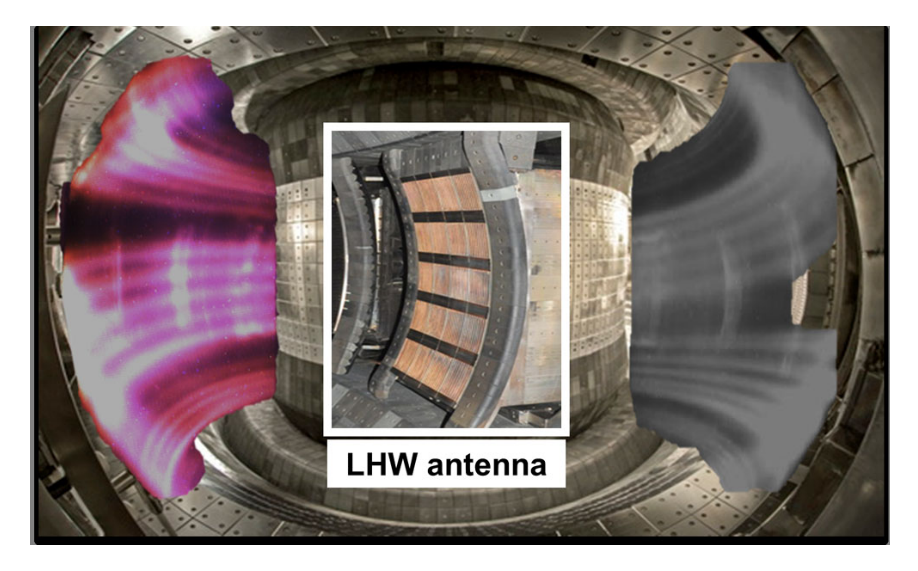
\includegraphics{hcf/hcf_visible_image.png}
        \caption{\east 以氦气放电实验来用可见光显著地表现螺旋电流丝的三维几何分布,低杂波天线截图置于图中间。}
    \end{subfigure}
    % \hspace{4em}%
    \begin{subfigure}{0.45\textwidth}
        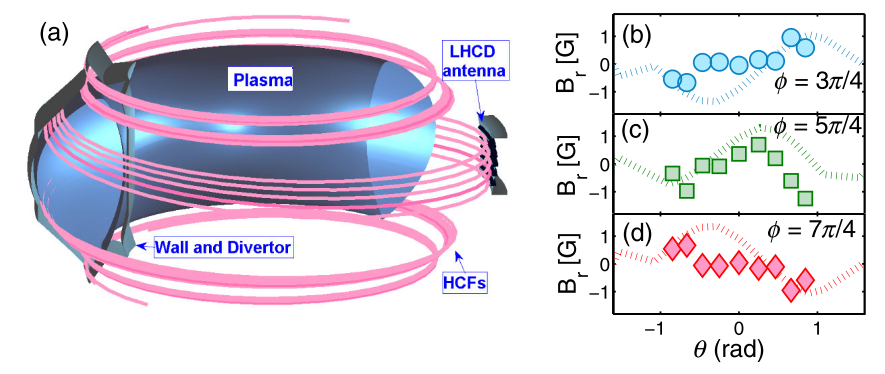
\includegraphics{hcf/hcf_model_sketch.png}
        \caption{对低杂波激发的螺旋电流丝以图 (a) 中的电流分布进行了模拟,计算结果得到环向非对称的磁扰动径向分布,图中显示了 (b) $\phi=3\pi/4$  (c) $\phi=5\pi/4$  (d) $\phi=7\pi/4$ 的计算和实验结果。极向角 $\phi$ 在低场侧赤道面为零顺时针方向增长;从上往下看托卡马克,环向角 $\phi$ 在低杂波天线处为零逆时针方向增长。}
    \end{subfigure}
    \caption{高 $m$ 线圈作用下的 \Poincare 图,次要工作模式下的磁扰动情况较主要模式更深,来源于张华祥研究员 \cite{zhang_highm} 的报告}
    \label{fig:highm-stretched-poincare}
\end{figure}
  

在 EAST 中为了研究低杂波及螺旋电流丝,以方波调制的低杂波功率进行了间断性的螺旋电流丝激励 \inlinecite{the_east_team_magnetic_2013}。低杂波天线运转时,螺旋电流丝引起的三维磁拓扑(磁连接长度计算如图 \ref{fig:hcf-connection}) 导致了粒子流三维分裂的落点图案。\cite{the_east_team_magnetic_2013}

\begin{figure}[htbp]
    \centering%
        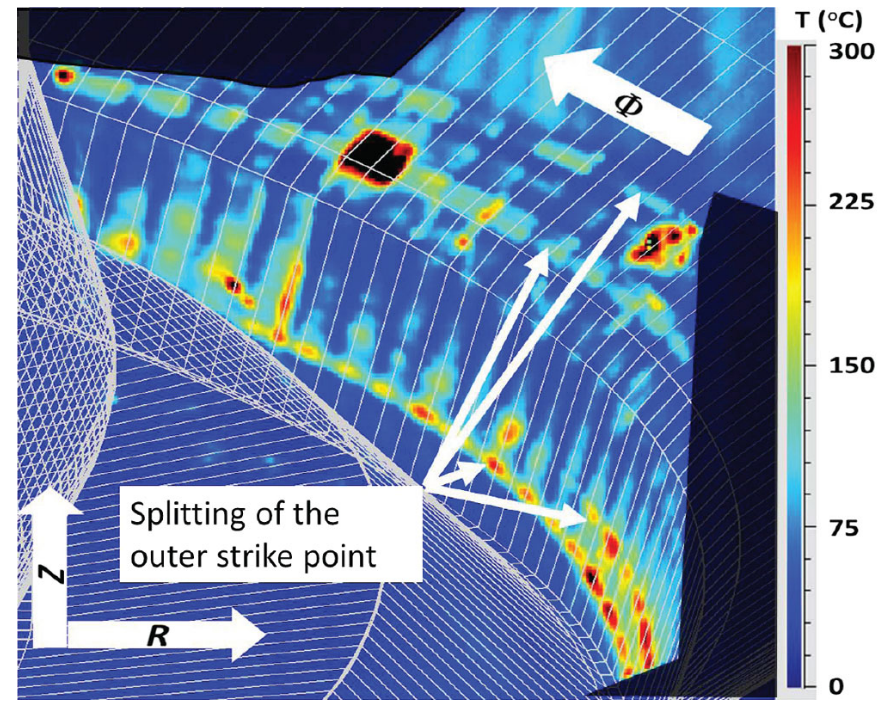
\includegraphics[height=9cm]{hcf/splitting_strike_point_ir.png}
        \caption{红外摄像机分析得到的\east 外侧偏滤器平板上$\phi=1.3\pi\sim 1.5\pi$低杂波运转时的温度分布。图中可见落点分裂为多个条状加热图案,还可以发现环向上分布的不对称性。腔壁网格重叠在图中以白线显示环形腔结构。}
        \label{fig:hcf-strike-point}
\end{figure}

\begin{figure}[htbp]
    \centering%
        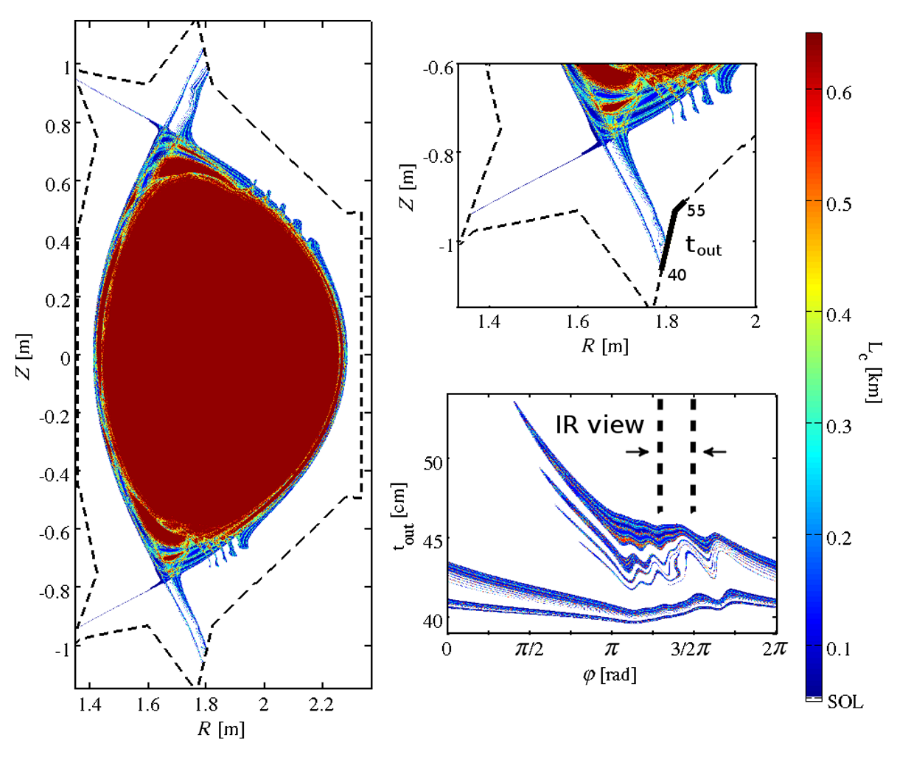
\includegraphics[height=9cm]{hcf/connection_contour.png}
        \caption{用上图 \ref{fig:hcf-strike-point} 实验中测量值重建的 \east 中磁连接长度在极向截面 $\phi=1.3\pi$ 上的等位线分布,其下偏滤器处的分布可见用右上小图。对落点的分布计算可见右下小图,右图 \ref{fig:hcf-strike-point} 红外拍照区域在小图中标注。}
        \label{fig:hcf-connection}
\end{figure}


\section{\Poincare 图及傅里叶模数分析}
\Poincare 图是对磁面结构的描述,通过在给定极向截面上进行沿磁力线的迭代来标记在同一磁面上的点,以描绘出磁面的嵌套结构。

\section{数值计算工具}
\subsection{有限元、有限体积法}
偏微分方程的求解问题构成了现代工程领域许多重要的设计工作,计算框架和数值理论在各种高性能计算处理器的基础上的组合计算成为了现代工业设计的重要设计及优化工作。

有限元法(Finite Element Method, FEM)在多物理场分析中很成功,一方面它非常通用,另一方面有限元可以对不同计算域内物理问题适合的算法进行组合,这对于多物理问题而言是一个关键优势。

尽管有限元可以自然地处理弯曲和不规则几何图形,但有限元背后的数学相对有限体积法(Finite Volume Method, FVM)更复杂一些。有限体积法中自然地对物理偏微分方程组中的守恒量进行在网格上进行积分,离散值表示的是单元内该守恒量的积分平均值。于是有限体积法的重点在于如何通过单元(cell)的积分平均值插值表示单元边界的守恒量流量,即流函数。

% 最后,对于时域时间上的仿真,为了效率往往需要使用显式求解器。但是有限元在实施此类技术方面存在困难,因此建议不要使用它。

\begin{itemize}
    \item 等离子体所采用的电磁场计算软件 TODO
    \item \textit{FEniCS\footnote{\url{https://fenicsproject.org/}}} 是开源(LGPLv3)的偏微分方程计算框架。 FEniCS 中丰富的 Python-C++ 接口使得科学工作者可以迅速地将他们面对的科学模型转化为有限元程序逻辑。在这里我们选取 FEniCS 是因为其后端的 PETSc\footnote{\url{https://www.mcs.anl.gov/petsc/}} 在支持 OpenMP、OpenCL 和 CUDA,在针对 PDE 的硬件优化上几乎无出其右,可以在几乎在任何并行计算硬件平台上得到快速应用。\underline{考虑到毕设时间的有限并且可能将考虑非线性等离子体响应},具备高层接口的 FEniCS 是快速实现偏微分方程的手段\inlinecite{FEniCS_LangtangenLogg2017}。
    \item \textit{SU2\footnote{\url{https://su2code.github.io}}} 工具箱是基于 C++ 偏微分方程的求解分析工具并可以在给定条件基础上进行设计优化。这套工具是为计算流体力学和空气动力学形状优化而设计的,但它也能够进行扩展来处理任意几何的控制方程,例如位势流,弹性问题,电流力学问题,化学反应流以及其他问题。
    \item \textit{MFEM\footnote{\url{https://mfem.org/}}} 与 FEniCS 类似,MFEM 也支持对后端采用 PETSc 进行并行加速。其在电磁场领域有过一些研究,在本论文中被采用作为辅助验证工具。
    \item \textit{\mdddc \footnote{\url{https://w3.pppl.gov/~nferraro/m3dc1.html}}} 由美国普林斯顿大学等离子体实验室开发,是一个聚变等离子体界影响深远的非线性双流体模拟计算工具。但由于中美关系恶化及其代码闭源问题,\mdddc 的数值高精度算法及各类成果在本论文中仅作为数值理论的参考。
\end{itemize}



以下为 \mdddc 中的双流体模型方程,其推导过程参见附录。TODO
\begin{equation}\begin{aligned}
    \frac{\partial n}{\partial t}+\nabla \cdot(n \vect{u})=& 0 \\
    n m_{i}\left(\frac{\partial \vect{u}}{\partial t}+\vect{u} \cdot \nabla \vect{u}\right)=& \vect{J} \times \vect{B}-\nabla p-\nabla \cdot\tens{\Pi}+\vect{F} \\
    \frac{\partial p}{\partial t}+\vect{u} \cdot \nabla p+\Gamma p \nabla \cdot \vect{u}=&(\Gamma-1)\left[Q-\nabla \cdot \vect{q}+\eta J^{2}-\vect{u} \cdot \vect{F}-\tens{\Pi}: \nabla u\right] \\
    &+\frac{1}{n e} \vect{J} \cdot\left(\frac{\nabla n}{n} p_{e}-\nabla p_{e}\right)+(\Gamma-1) \tens{\Pi}_{e}: \nabla\left(\frac{1}{n e} \vect{J}\right) \\
    \frac{\partial p_{e}}{\partial t}+\vect{u} \cdot \nabla p_{e}+\Gamma p_{e} \nabla \cdot \vect{u}=&(\Gamma-1)\left[Q_{e}-\vect{q}_{e}+\eta J^{2}-\vect{u} \cdot \vect{F}_{e}-\tens{\Pi}_{e}: \nabla u\right] \\
    &+\frac{1}{n e} \vect{J} \cdot\left(\frac{\nabla n}{n} p_{e}-\nabla p_{e}\right)+(\Gamma-1)\left[\tens{\Pi}_{e}: \nabla\left(\frac{1}{n e} \vect{J}\right)+\frac{1}{n e} \vect{J} \cdot \vect{F}_{e}\right]
\end{aligned}\end{equation}

\begin{table}[htb]
    \centering
    % \caption[模板文件]{模板文件。如果表格的标题很长,那么在表格索引中就会很不美
    %   观,所以要像 chapter 那样在前面用中括号写一个简短的标题。这个标题会出现在索
    %   引中。}
    \label{tab:formula_double-fluid}
    \begin{tabularx}{\linewidth}{lXlXlX}
        % \toprule[1.5pt]
        $p,p_e$ &  总/电子压强 & $\vect{q}$ & 热流密度 & $\vect{J}$ & 电流密度\\
        $\tens{\Pi},\tens{\Pi}_e$ & 总/电子粘性系数 &$u$ & 流体速度 & $n$ & 粒子数密度 \\
        $\vect{F},\vect{F}_e$ & &$\tens{\Pi}$ & & $Q,Q_e$ & 
        % \midrule[1pt]
        % \bottomrule[1.5pt]
    \end{tabularx}
\end{table}

\begin{equation}
\vect{E}=\eta \vect{J}-\vect{u} \times \vect{B}+\frac{1}{n e}\left(\vect{J} \times \vect{B}-\nabla p_{e}-\nabla \cdot \tens{\Pi}_{e}+\vect{F}_{e}\right)\end{equation}

\begin{equation}\begin{aligned}
    \vect{J} &=\frac{1}{\mu_{0}} \nabla \times \vect{B} \\
    \frac{\partial \vect{B}}{\partial t} &=-\nabla \times \vect{E}
\end{aligned}\end{equation}

\mdddc 中还有单流体模型, \cite{canal_m3d-c1_2017} 对 NSTX-U 中等离子体对扰动场的响应做了稳态单/双流体模拟的对比。

\begin{equation}\begin{aligned}
    \nabla \cdot\left(n \vect{v}_{\mathrm{i}}\right)=&0\\
    m_{\mathrm{i}} n \vect{v}_{\mathrm{i}} \cdot \nabla \vect{v}_{\mathrm{i}}=&\vect{J} \times \vect{B}-\nabla p-\nabla \cdot \tens{\Pi}_{\mathrm{i}}\\
    \frac{\nabla \cdot\left(p \vect{v}_{\mathrm{i}}\right)}{\Gamma-1}+p \nabla \cdot \vect{v}_{\mathrm{i}}+\nabla \cdot \vect{q}=&\eta J^{2}-\tens{\Pi}_{\mathrm{i}}: \nabla \vect{v}_{\mathrm{i}}-\frac{\vect{J}}{n e(\Gamma-1)} \cdot\left(\Gamma p_{\mathrm{e}} \frac{\nabla n}{n}-\nabla p_{\mathrm{e}}\right)\\
    \nabla \times \vect{E}=&0\\
    \nabla \times \vect{B}=&\mu_{0} \vect{J}
\end{aligned}\end{equation}

\begin{equation}\vect{E}=\eta \vect{J}-\vect{v}_{\mathrm{i}} \times \vect{B}+\frac{1}{n e}\left(\vect{J} \times \vect{B}-\nabla p_{\mathrm{e}}\right)\end{equation}

\begin{equation}\tens{\Pi}_{i}=-\mu_{i}\left[\nabla \vect{v}_{i}+\left(\nabla \vect{v}_{i}\right)^{t}\right]\end{equation}

\begin{equation}\vect{q}=-\kappa \nabla\left(T_{e}+T_{\mathrm{i}}\right)-\kappa_{\|} \vect{B}\left(\vect{B} \cdot \nabla T_{\mathrm{e}}\right) / B^{2}\end{equation}

\subsection{质点网格法 Particel-in-cell (PIC)}

在以上的偏微分方程求解时,物理问题允许将某一点(或一个邻域内)的物理量取其代表值来离散化,如有限体积法中取其网格内的平均值进行计算,,有限元法中取有限阶多项式逼近。然而,在并不一定完全服从高斯速度分布的等离子体物理研究中,这样的代表值很难抽取出来。类似的非高斯型速度分布导致的流体假设不成立的问题,在裂变堆中子物理计算中采用的是多群计算的方法;而在聚变等离子体物理问题中,不论是自然产生的等离子体还是人工产生的加速器,往往会出现相当各向异性的速度分布,以至于需要细致地考虑在相空间中求解。对粒子在相空间(Phase space)中的分布函数 $f(\vec{x},\vec{v},t)$,描述其演化规律的物理方程是 Boltzmann 方程,\cite{ColonnaBoltamann10.1088/978-0-7503-1200-4ch1}.

\begin{equation}
\label{eq:Boltzmann}
\frac{\partial f_{s}(\vec{r}, \vec{v}, t)}{\partial t}+\left[\vec{v} \cdot \nabla_{r}+\vec{a}(\vec{r}) \cdot \nabla_{v}\right] f_{s}(\vec{r}, \vec{v}, t)=\left(\frac{\delta f_{s}}{\delta t}\right)_{\mathrm{coll}}
\end{equation}

其中 $(\delta f_{s}/\delta t )_{\mathrm{coll}}$ 表示同种粒子及不同粒子之间的相互碰撞导致的粒子 s 的 $f_s$ 变化率。
Particle-in-cell, 即 PIC 手段将电磁场进行常规的偏微分方程求解,另外,还令网格中分布着巨粒子。巨粒子对网格角点处的电磁场参数数值有所影响,同时巨粒子也会根据离散的电磁场计算其下一时间步长的速度和坐标,这样就一定程度上在完全的粒子模拟和有限网格计算方法之间达到所需要的性能、准确之间的平衡。

\subsection{磁力线定迹}
针对聚变磁约束中的磁力线定迹问题 (field-line-tracing) 和射线定迹问题 (ray-line-tracing) ,相空间中的复杂计算可以在 PIC 基础上根据磁约束的特点进行简化。以下介绍 CompX \footnote{
Computational Modeling and Software Development\url{http://compxco.com/index.html}}项目中的代码 GENRAY 和 CQL3D\footnote{它们实在太古老了,如果可以的还是把它们用 C++ 重写一遍吧}。项目中用它们作为磁力线定迹的工具。

\subsubsection{GENRAY}
GENRAY 通过几何光学式的折射处理对射线进行迹线追踪和强度变化的检索。


\subsubsection{CQL3D (Collisional QuasiLinear 3 D)}

\begin{multline}
\frac{d f}{d t}=\text{total derivative following the particle guiding center,}
=\frac{\partial f}{\partial t}+\underline{v}_{\mathrm{g.c.}} \cdot \frac{\partial f}{\partial \underline{r}}+\frac{\partial f}{\partial \mu} \frac{d \mu}{d t}+\frac{\partial f}{\partial \varepsilon} \frac{d \varepsilon}{d t}
\end{multline}


\begin{equation}\frac{d f}{d t}=\frac{\partial f}{\partial t}+v_{\|} \hat{b} \cdot \nabla f+q E_{\|} v_{\|} \frac{\partial f}{\partial \varepsilon}+O(\delta)\end{equation}

\section{磁流体不稳定性}
磁流体不稳定性高度依赖于其边界磁面的螺旋形态,而为了阐述磁面的螺旋度,旋转变换的相关知识是必需的。\textbf{旋转变换}(rotational transform, 本质上是磁面磁力线螺距角)的定义是磁力线绕环向方向转一圈时极向绕小半径转的圈数。假如磁面是互相嵌套的话,旋转变换率在磁面上的平均值由极向磁通随环向磁通的变化率决定。
$ \iota/2 \pi = d\Psi /d \Phi $。

但托卡马克中,其倒数 \textbf{安全因子} 却更常被使用,$q = 2\pi/\iota$。在截面圆形,主要由等离子体电流产生极向场的托卡马克中磁力线的方程近似满足 $ \frac{r d\theta}{B_\theta} = \frac{Rd\phi}{B_\phi} $,
其中 $ \phi $ and $\theta$ 分别是环向角和极向角。 于是在典型的托卡马克中, $ q = m/n = \left \langle d\phi /d\theta \right \rangle $ 可以用 $ q \simeq \frac{r B_\varphi}{R B_\theta} $ 近似。如果磁面安全因子 $q\leq 2$,边界上会发生显著的磁流体不稳定性。

在带偏滤器的托卡马克中,$q$ 在等离子体分界面某些部分趋近无穷,所以通常会考虑在分界面内侧的 $q$,通常来说会选 95\% 的磁面 (内部磁通占总环向磁通的 95\%), 此时常用 $q_{95}$ 来表示.




​\section{主要目标}
为了探究解决目前的\Hmode 等离子体所面临的 ELM 脉冲式热流和粒子流问题,而这在 DEMO 堆中是不被允许的。

为更好地控制 ELM, EAST 上先后测试了共振磁扰动线圈 RMP、高 m 线圈和低杂波驱动的螺旋电流丝,这三种扰动场产生机制有所差异,适用的范围也不尽相同。为了使扰动场相互配合达到最优的弱化乃至抑制边界局域模的效果,对它们在等离子体边界造成的扰动场协同作用的研究是很有必要的。 \textit{\textbf{(1)}} \textbf{腔内低场侧低 $n$ 线圈},该线圈布置在腔内,由它激发起环向模数为 $n=1,2$ 的扰动场后在 \east, \ddd 等托卡马克装置上验证了其抑制边界局域模的效应。 \textit{\textbf{(2)}} \textbf{高 m 线圈},是 EAST 团队近两年实验中的线圈,在等离子体环外加上一组四个的线圈,它的特征是扰动场环向模数 n 分布较宽,极向模数 m 较高,由于只分布在一个环向位置 $\varphi=\text{const}$,扰动场的局域性很强。 \textit{\textbf{(3)}} 由低杂波驱动的\textbf{螺旋电流丝},低杂波原本用于以朗道阻尼驱动芯部等离子体的电流,但在设计之外,实验发现它在等离子体边界会激发出螺旋电流丝,电流丝产生具体的物理机制还不甚明晰,但其亦具备调节边界磁拓扑的能力。由于低杂波天线不像共振磁扰动线圈在腔内,它具有应用在 DEMO 堆及日后商业堆的潜力。

本文将会对边界磁拓扑在扰动场作用下的变化做出(磁流体)电磁分析,绘制近边界磁面的傅里叶谱和 \Poincare 图,这构成了第二章的主要内容。在此之后,第三章将基于磁场弥散来进行粒子扩散的模拟,对粒子在边界上的运动建立直观的认识,通过修改 GENRAY-CQL3D 磁力线定迹程序可以较原来的模型更为精确。通过前面提到的多种扰动场对等离子体边界拓扑进行调节,从而对热负荷和粒子流在偏滤器上的分布进行优化,以避免脉冲式的 ELM 崩溃对壁材料造成显著的影响。最后,(如果还有时间的话Optional),通过在模拟工具中引入等离子体反馈后的随机场的计算,从而在湍流输运的角度解释磁场边界拓扑对粒子输运和热流的影响。

本论文着重在通过模拟的手段对现有的多种三维磁场进行模拟仿真,他们的磁谱被设计用来弱化或者调节边界局域模的发生。但他们之间的同时作用可以如何达到对粒子束流和热流的调节作用。
\chapter{扰动场协同优化}

\section{协同模拟中的磁谱计算简化理论}
FLT 在最外闭合磁面的水平方向外平移 10 mm, FLT 会从下沿进入强场侧,为避免这种情况,向外平移 15 mm 余。
% \begin{figure}[t]
%   \centering

%   \subcaptionbox{基于磁力线追踪计算得到的螺旋电流丝轨迹,五条分别螺旋电流丝起点分别取为五排低杂波天线的中间位置正对着的闭合磁面外 10 mm 以内。}{%
%     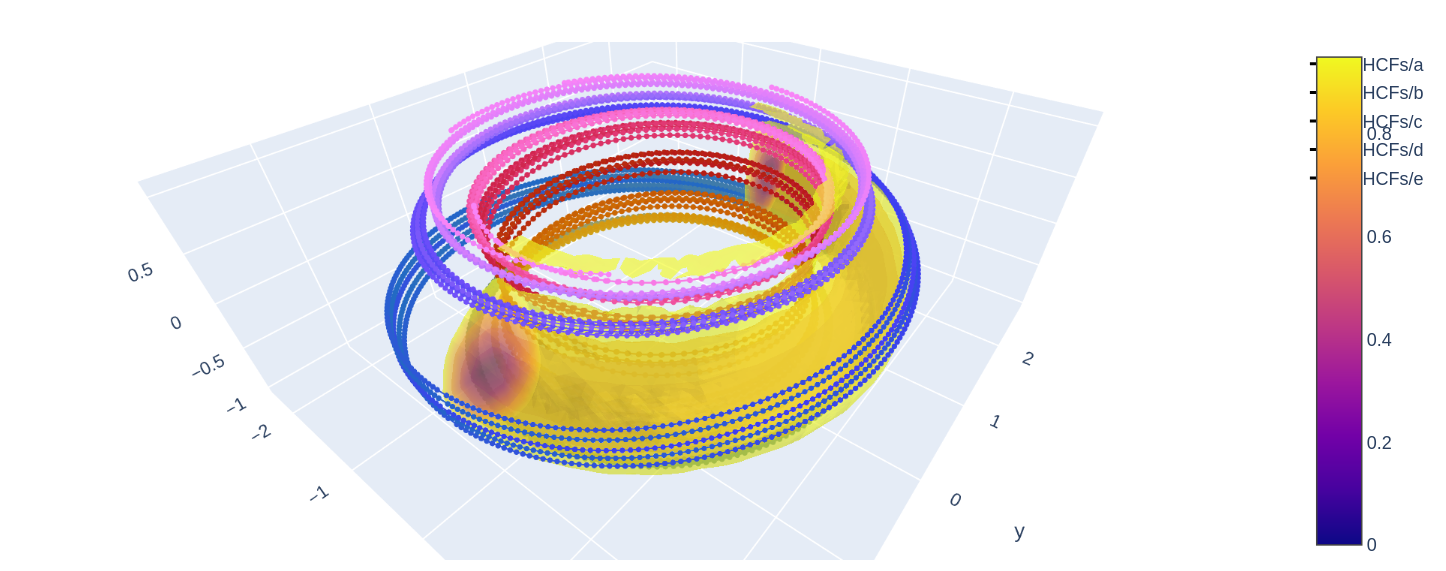
\includegraphics[width=0.47\columnwidth,keepaspectratio]{73999_030400ms_improved/hcfs_east.png}
%   }\hfill
%   \subcaptionbox{\east 上 RMP 线圈(低 n 线圈)、高 m 线圈及在闭合磁面外 15 mm 余处开始延伸的螺旋电流丝结构图。}{%
%   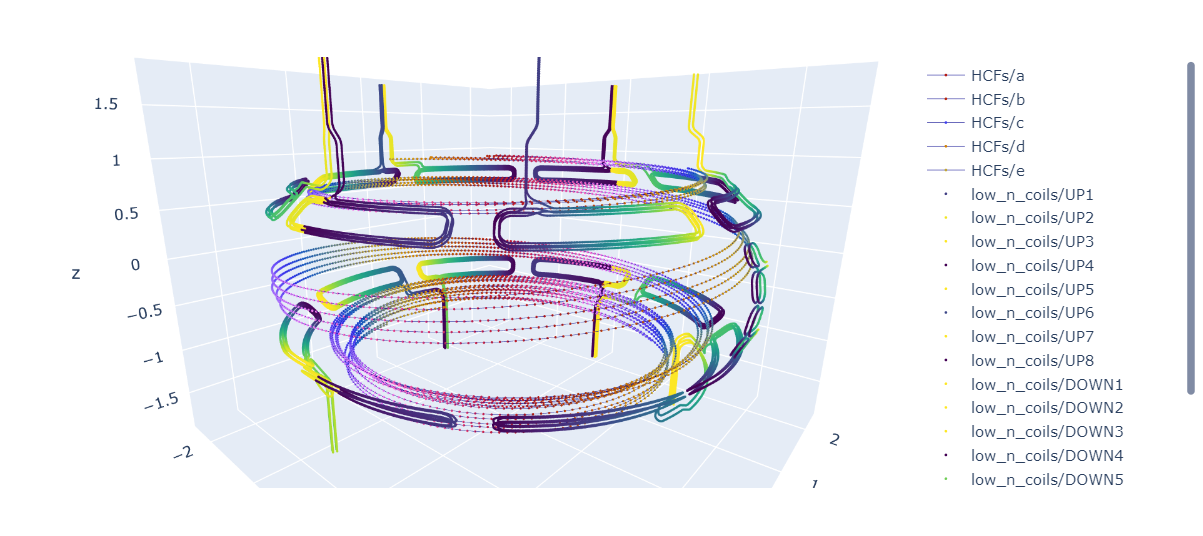
\includegraphics[width=0.47\columnwidth,keepaspectratio]{visual_coilsys.png}
% }
% \end{figure}

  高 m 线圈在 $\varphi$ 正方向上进行移动 $\Delta \varphi$,相当于$\tilde{b}_{m n}^{1}(s)$乘因子 $e^{-i\left(n \Delta\varphi \right )}$。

  下表罗列除了线圈电流幅值、相位及线圈位置等可调参数的可选空间。
  螺旋电流丝的电流强度和位置实验上不太好控制,暂时将其作为给定量,由其他线圈配合它。

  
\begin{table}[htb]
  \centering
  \caption{扰动场可调参量}
  \label{tab:east_parameter}
  \begin{tabularx}{\linewidth}{lXX}
      \toprule[1.5pt]
      变量 & 备注 & 可选区域 \\
      \midrule[1pt]
      $I_{amp~\text{UP}}$ & RMP 线圈上沿电流幅值 & $[-10 \text{kAt}, 10 \text{kAt}]$\\ 
      $I_{amp~\text{DOWN}}$ & RMP 线圈下沿电流幅值 & $[-10 \text{kAt}, 10 \text{kAt}]$\\ 
      $I_{amp~\text{high m, UP}}$ & 高 $m$ 线圈上沿电流幅值 & $[-10 \text{kAt}, 10 \text{kAt}]$\\
      $I_{amp~\text{high m, DOWN}}$ & 高 $m$ 线圈下沿电流幅值 & $[-10 \text{kAt}, 10 \text{kAt}]$\\
      $\Phi_{UP}$ & RMP 线圈上沿电流相位 & $[-\pi, \pi]$\\
      $\Phi_{DOWN}$ & RMP 线圈下沿电流相位 & $[-\pi, \pi]$\\
      $\phi_{\text{high m}}$ & 高 m 线圈环向分布角 & $[-\pi, \pi]$\\
      \bottomrule[1.5pt]
  \end{tabularx}
\end{table}
  
傅里叶变换的线性性、平移性大大减少了计算磁谱的成本。

  \begin{itemize}
    \item 线性性:线圈强度的变化,利用傅里叶变换的线性性减少计算量。
    \item 平移性:高 m 线圈的角度是指其自身物理位置在柱坐标系统沿中心轴进行环向上的旋转的角度,在 $(\theta^*, \varphi)$ 上沿着 $\varphi$ 平移 $\Delta\varphi$,利用傅里叶变换的平移性质,相当于$\tilde{b}_{m n}^{1}(s)$乘因子 $e^{-i\left(n \Delta\varphi \right )}$,。
    $$\Delta\varphi \Rightarrow e^{-i\left(n \Delta\varphi \right )}$$ 类似的,如果在极向角度上改变 $\Delta\theta^*$,则可以乘因子 $e^{-i\left(n \Delta\theta^* \right )}$。
  \end{itemize}  
  


\subsection{优化函数}

    
    这是偏工程方面的优化问题,目标函数有两个条件。一个是尽可能地生成强的边界随机场,这一方面我们用 Chirikov 参数来刻画;另一方面是希望新经典环向粘滞的影响尽可能地小,我们下面给出下面的评估标准。
    
  品质因子定义 (figure of merit, FoM),
  
  \begin{equation}
    FoM=\left[\frac{\langle\sigma\rangle_{s_{1}<s<s_{2}}^{4}}{\left\langle\sum_{m, n(n \neq 0)}\left[b_{m n}^{r}\right]^{2}\right\rangle_{s_{3}<s<s_{4}}}\right]
  \end{equation}
  
\begin{equation}
  b^r = \frac{\vect{B}\cdot\vect{n}}{B_0} = \frac{\vect{B}\cdot \nabla s}{B_0 |\nabla s|}
\end{equation}

我们同样对 $b^r$ 做类似 $\tilde{b}^1$ 的 Fourier 变换

\begin{equation}
  b_{m n}^{r}(s) \equiv \int_{\varphi=0}^{2 \pi} \int_{\theta^{*}=0}^{2 \pi} b^{r}\left(s, \theta^{*}, \varphi\right) e^{-i\left(m \theta^{*}+n \varphi\right)} \frac{d \theta^{*}}{2 \pi} \frac{d \varphi}{2 \pi}
\end{equation}

\begin{equation}
  b^{r}\left(s, \theta^{*}, \varphi\right)=\sum_{m, n=-\infty}^{\infty} b_{m n}^{r}(s) e^{i\left(m \theta^{*}+n \varphi\right)}
\end{equation}

  
其中分母是 $b^r$ 磁谱中分量平方的加和,用它来定性刻画新经典环向粘滞(Neoclassical Toroidal Viscosity, NTV)影响大小。当托卡马克的环向对称性被打破时,会有额外的力矩作用在等离子体上,从而形成共振的环向旋转频率,这被称为新经典粘滞效应。

当只考虑基频分量引起的磁岛时时,$\sigma\propto \sqrt{I_{coil}}$,Chirikov 参数与扰动场幅值成正比,而$b^r_{mn}\propto I_{coil}$,故而 Chirikov 参数取四次幂作为分子,从而扰动场的幅度变化不会影响该品质因子。
% 香蕉粒子在等离子体中以香蕉状轨迹往复运动导致的额外的粘性。


% 而关于

% $\tilde{b}_{r e s}^{1}$ The expression that we use for the physical effective radial RMPs is:
% \[
% b_{r e s}^{r} \equiv \frac{\tilde{b}_{r e s}^{1}}{R_{0}\langle\sqrt{g^{11}}\rangle_{\theta^{*}}}
% \]
% where the brackets represent an averaging over $\theta^{*}:\langle\sqrt{g^{11}}\rangle_{\theta^{*}} \equiv \int_{\theta^{*}=0}^{2 \pi} \sqrt{g^{11} \frac{d \theta^{*}}{2 \pi}} .$ 


  % \begin{enumerate}
  %   \item 在边界共振分量较大为好,越在边界产生的共振分量越重要,积分权重与到有理面共振线的距离成反比 $d=dist(point(n,m),q(\Psi_{pol})n)\downarrow, \rho(m,n,q) \uparrow$。
  %   \item 减去或除去芯部有理面的共振分量,减弱 2/1, 3/1 有理面存在的不稳定性反馈。。
  % \end{enumerate}
    
  % \begin{equation}
  %   \int_{\Psi_{pol}>0.87} \sum_{m,n} \rho(m,n,q) |B_{mn}^r| S(\Psi_{pol})d\Psi_{pol} - \sum_{internal~\Psi_{pol}} \sum_{m,n} \rho(m,n,q) |B_{mn}^r|
  % \end{equation}
  
  % 确定了优化函数后通过共轭梯度法找到一个较优解,或者算力允许的话画等位图。
  
    
  % 取磁面坐标$(s=\Psi^{1/2}_{pol},\theta^*,\varphi)$,


    
  
    




\section{扰动场协同模拟结果}
在协同模拟实验中,各扰动场在对应的场源为 \SI{1}{\kilo\ampere t} 时的扰动场被保存为场数据文件。标记各扰动场源正方向,\textit{(1) RMP 线圈 / 低 n 线圈} 产生的 $B^1$ 在作用的核心区为正即为正  \textit{(2) 高 m 线圈} 确定主要工作模式 $B^1$ 从上至下是 -,+,-,+ 分布,次要工作模式是 -,+,-; \textit{(3) 螺旋电流丝} FLT 电流沿磁场方向即为正方向

\subsection{三者扰动场共同作用}
  
  当首次进行实验时使三种扰动场同时加入到计算中中发现的一些问题。

  
     对于单零位型,上下两侧扰动场线圈产生的扰动场大小明显不同,使得电流相对大小参与到优化中更有必要。

     近期磁谱优化的试验发现,磁谱 $\tilde{b}^1_{mn}$ 的脊线和磁面安全因子对应的曲线贴合程度不足,HCFs 产生的磁场作为基底磁场的影响过大。
    HCFs 基底磁场对应的 figure of Merit 已经达到 $3.56 * 10^7$, 优化后可以达到 $4.11 * 10^7$,但倍增的系数不大,意义不是很明显,RMP 线圈没有怎么发挥作用。令人吃惊的是不合适地选取 RMP 和 高 m 线圈的各项参数可能导致该值降到 $10^5$ 的量级。 

    


  





  \begin{figure}[t]
    \centering
    % \subcaptionbox{三种线圈共同优化后的结果,在 EAST 73999 Shot 上的 $|\tilde{b}^1_{m,n=-2}|$ 。}{%
      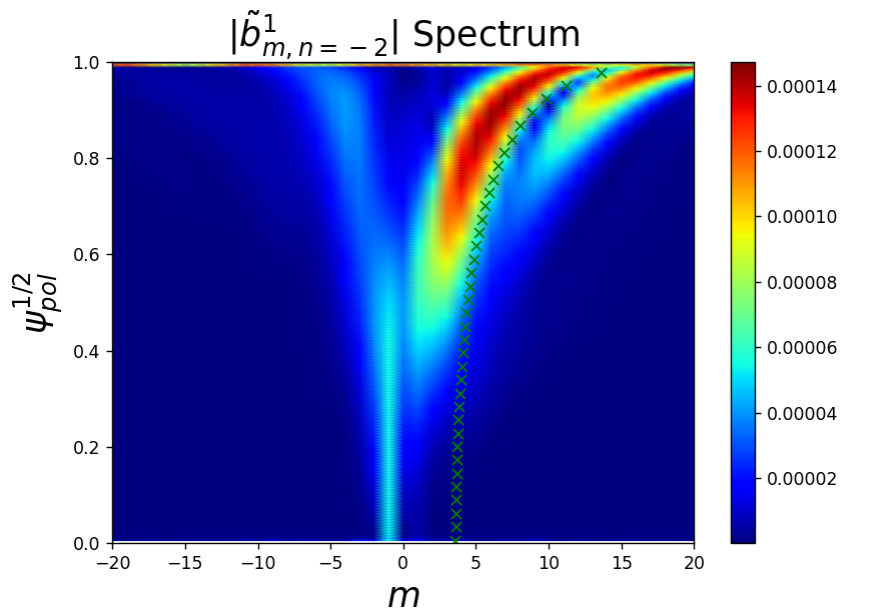
\includegraphics[width=0.7\columnwidth,keepaspectratio]{collab/collab_n=-2_b_sm_nfix_abs.PNG}
    % }
    % \hfill
    % \subcaptionbox{三种线圈共同优化后的结果,在 EAST 73999 Shot 上的 $\tilde{b}^1_{m,n=-2}$ 的相位分布。}{%
    %   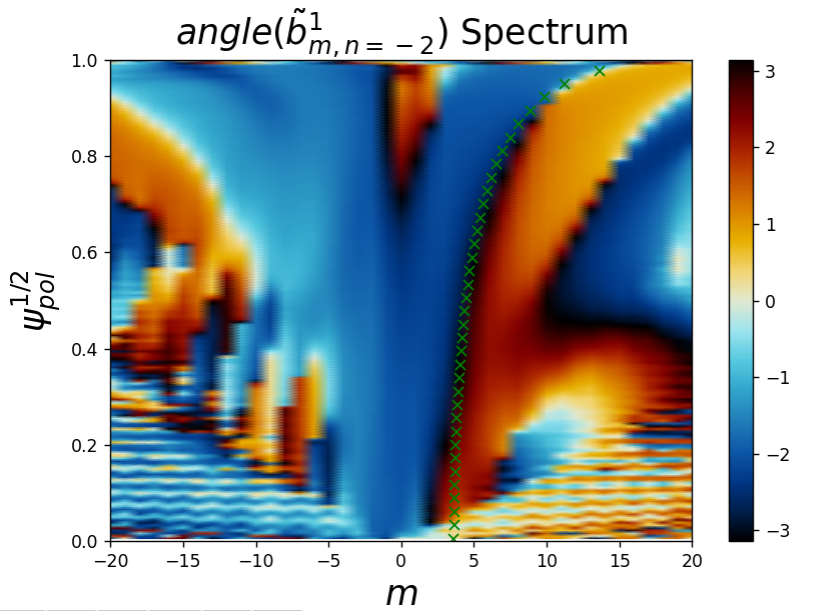
\includegraphics[width=0.47\columnwidth,keepaspectratio]{collab/collab_n=-2_b_sm_nfix_angle.PNG}
    % }%
    \caption{三种线圈共同优化后的结果,在 EAST 73999 Shot 上的 $|\tilde{b}^1_{m,n=-2}|$ 。}
  \end{figure}
  


  
  一开始尝试通过 python 科学计算库 scipy.optimize 函数进行优化得到极值, 但结果中 RMP 线圈的电流值常常在 1 kAt 以下,但高 m 线圈倒是较大,起始以为是陷入了局部极值,随后用了全局随机遍历发现得到的最大值,其对应的磁谱也与上面计算的结果类似,且 RMP 线圈优化得到的电流仍然小于 1 kAt。
  
  

  \begin{figure}[t]
    \centering
    % \subcaptionbox{两种线圈共同优化后的结果,在 EAST 73999 Shot 上的 $\tilde{b}^1_{m,n=-2}$ 的绝对值分布。}{%
      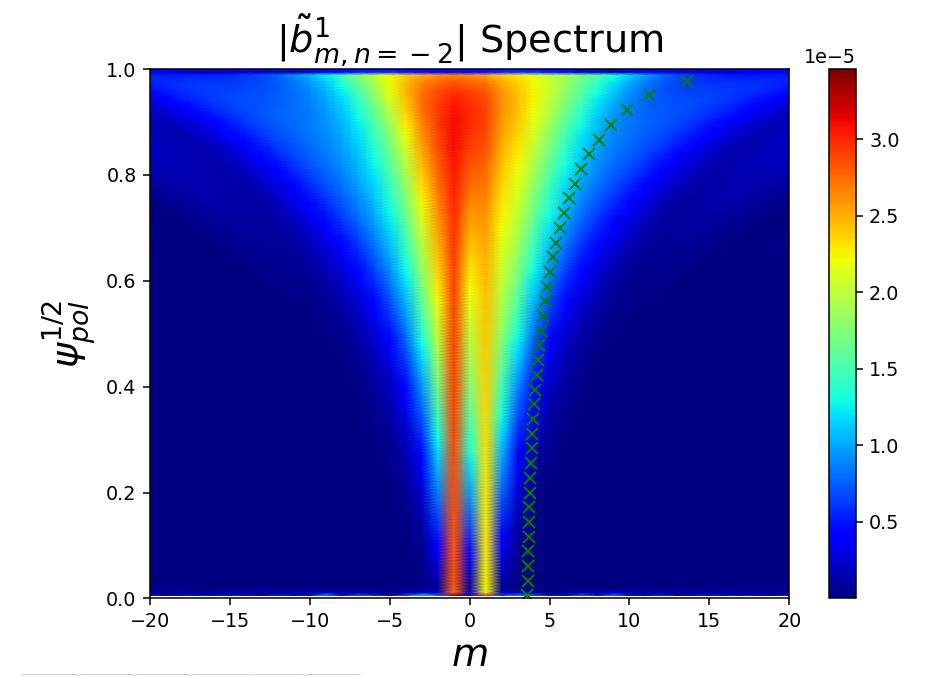
\includegraphics[width=0.7\columnwidth,keepaspectratio]{collab/collab_noHCFs_n=-2_b_sm_nfix_abs.PNG}
    % }%\hfill
    % \subcaptionbox{两种线圈共同优化后的结果,在 EAST 73999 Shot 上的 $\tilde{b}^1_{m,n=-2}$ 的相位分布。}{%
    %   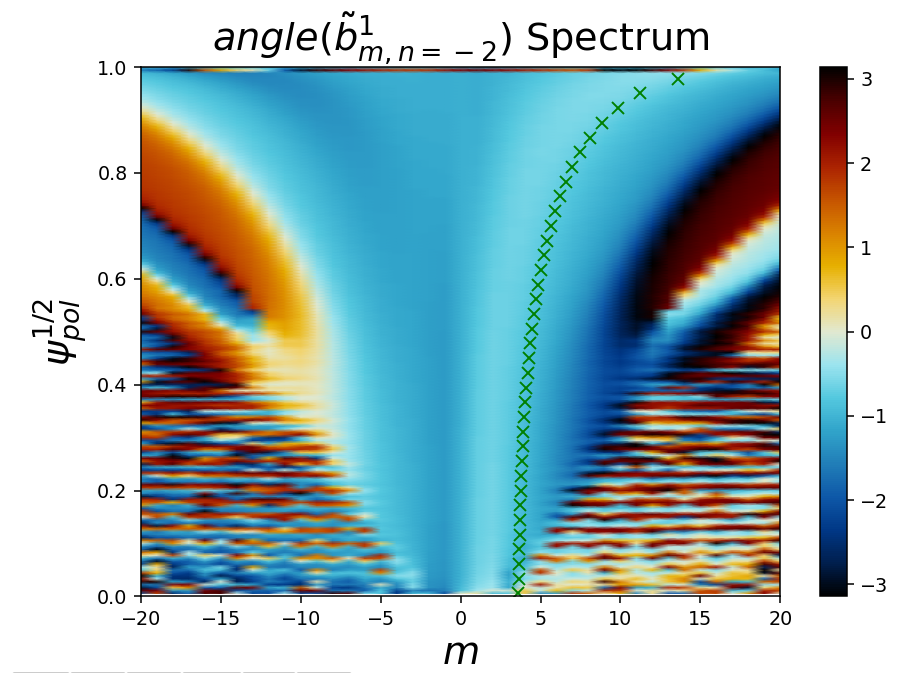
\includegraphics[width=0.47\columnwidth,keepaspectratio]{collab/collab_noHCFs_n=-2_b_sm_nfix_angle.PNG}
    % }%
    \caption{两种线圈共同优化后的结果,在 EAST 73999 Shot 上的 $\tilde{b}^1_{m,n=-2}$ 的绝对值分布。}
  \end{figure}
  
  随机得到的优化值中 RMP 线圈的电流值在 0.1 kAt 以下(高 m 线圈 -9.01486676 kAt),引起了我们进一步的探索。
  
  
  
\begin{figure}[t]
\centering
\label{fig:kAt-FoM}
\subcaptionbox{RMP UP 线圈 kAt 数 - FoM 散点图}{
    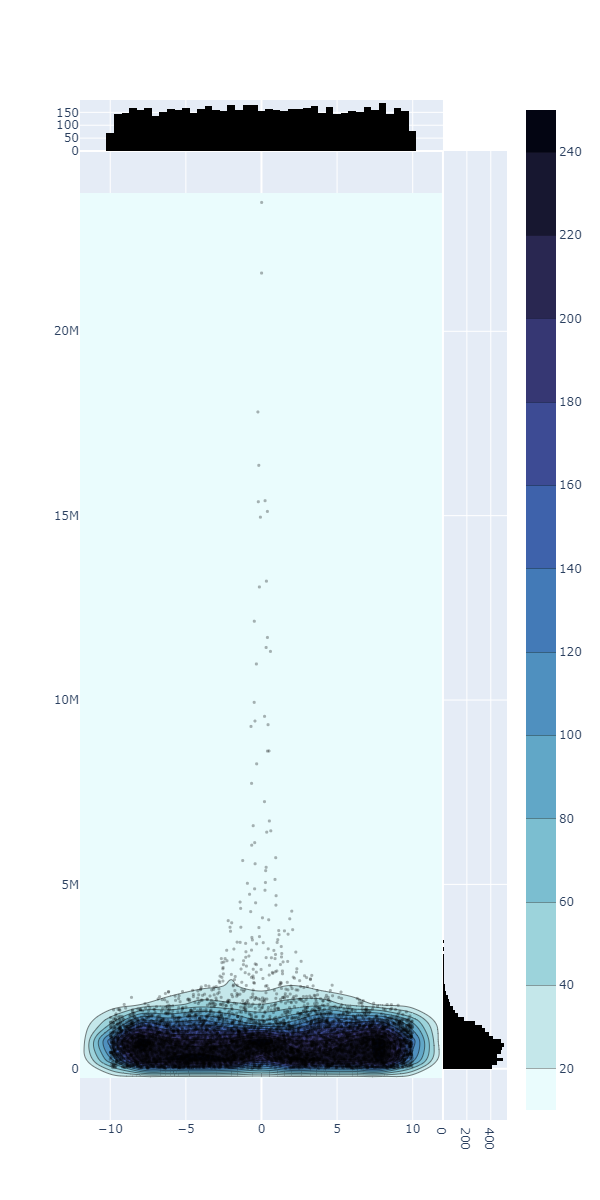
\includegraphics[width=0.32\columnwidth,keepaspectratio]{collab/low_n_UP_FoM.png}
}%\hfill
\subcaptionbox{RMP DOWN 线圈 kAt 数 - FoM 散点图}{
    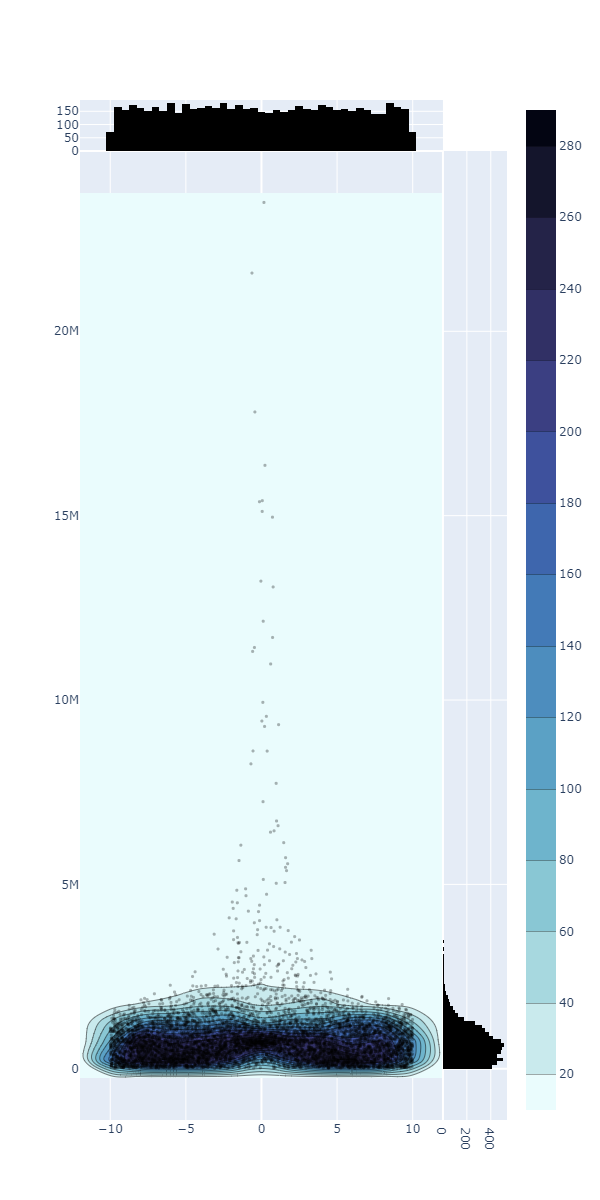
\includegraphics[width=0.32\columnwidth,keepaspectratio]{collab/low_n_DOWN_FoM.png}
}%\hfill
\subcaptionbox{高 m 线圈 kAt 数 - FoM 散点图}{
    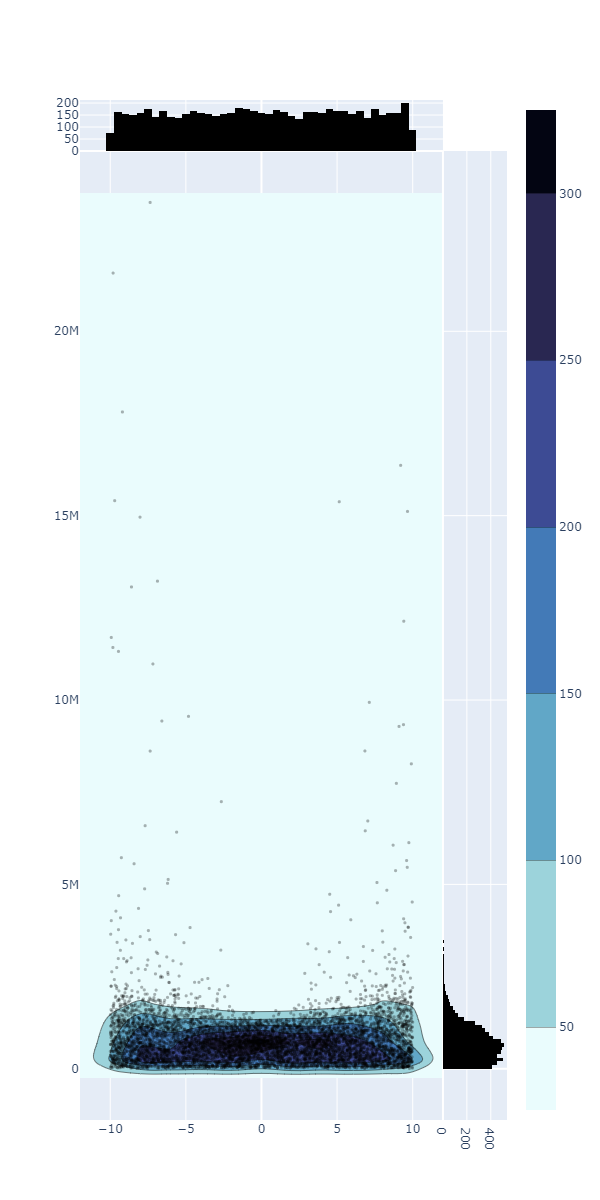
\includegraphics[width=0.32\columnwidth,keepaspectratio]{collab/high_m_FoM.png}
}
\caption{三种线圈电流幅值对品质因子影响的估计}
\end{figure}
  
  

线圈电流幅度对品质因子的影响参见上面几幅图,明显地有着 kAt 数较低 RMP 线圈和较高 kAt 数的高 m 线圈配合有可能产生较高的 FoM 的趋势,。RMP 线圈相位及高 m 线圈旋转角度三者作为坐标轴后作类似上图,未发现明显变化趋势。
  

高 m 线圈的电流幅度的增大会导致高 FoM 时 RMP 线圈的电流幅值容许范围得以增大。
  
  
% \begin{figure}[htbp]
%   \centering%
%       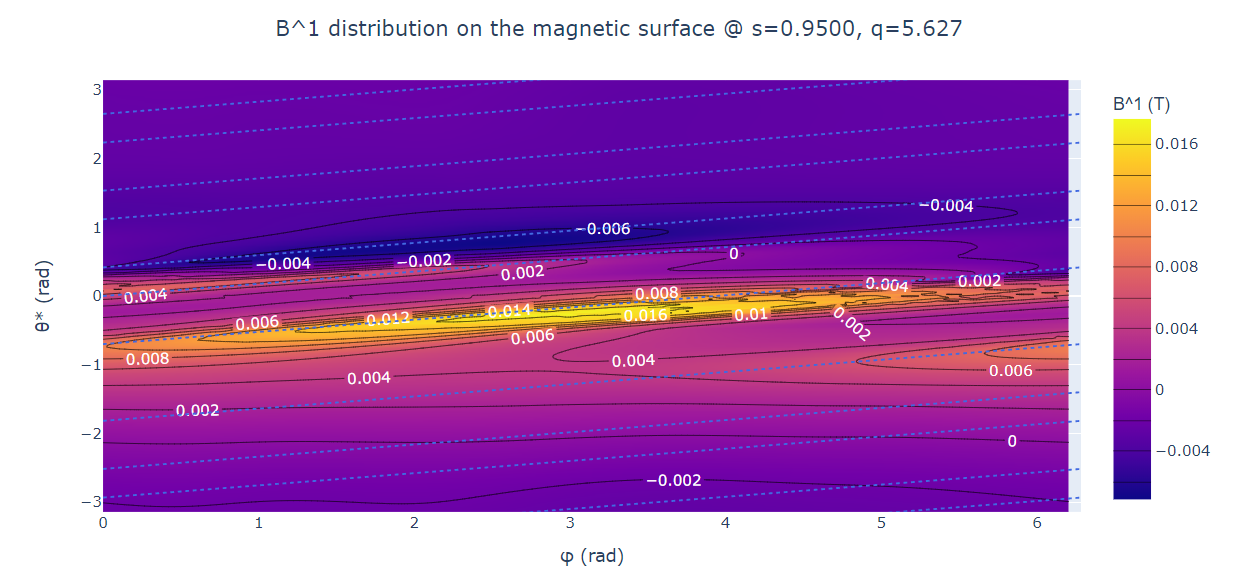
\includegraphics[width=1.0\columnwidth]{hcf/HCFs_uniform.png}
%       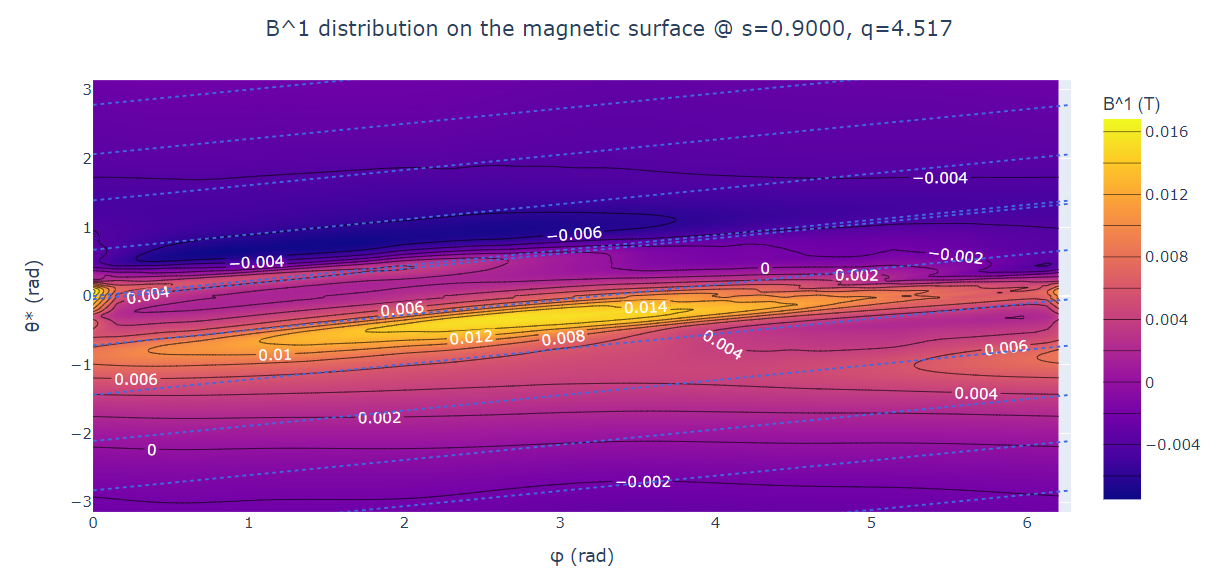
\includegraphics[width=1.0\columnwidth]{collab/collab_n=-2.PNG}
%       \caption{上下图分别为 HCFs 产生的基底磁场和三种扰动场优化后的磁场,各自的 $B^1$ 在磁面上 $s=0.950,0.900$ 的分布。虽然没有控制在一个磁面上,但可见优化后对磁场的影响并不大。}
% \end{figure}
  
  \begin{itemize}
    \item HCFs 产生的磁场太强,忽略它产生的基底磁场重新测试或者增大 RMP、高 m 线圈电流幅值允许范围。
    \item 在 HCFs 的影响下,磁谱脊线并没有向磁面螺旋度对应的曲线靠拢,反倒是原本的脊线最高值变得更高了。 
  \end{itemize}


在上述的问题出现之后,把螺旋电流丝搁置,先研究低 n (RMP) 线圈和高 m 线圈。


\subsection{RMP 线圈与高 $m$ 线圈扰动场共同作用}
随机得到的优化值中 RMP 线圈的电流值在 0.1 kAt 以下(高 m 线圈 -9.01486676 kAt),这意味着和高 m 线圈相耦合的低 n 线圈强度不能过高。该数值实验能帮助我们找到合适的扰动场匹配的大小,比如低 n 线圈(16个)和高 m 线圈(1个)在磁面上的磁通量有数量级的差异,它们应该在磁通量级可比时品质因子有个较好的结果。

\begin{figure}[htbp]
  \centering%
      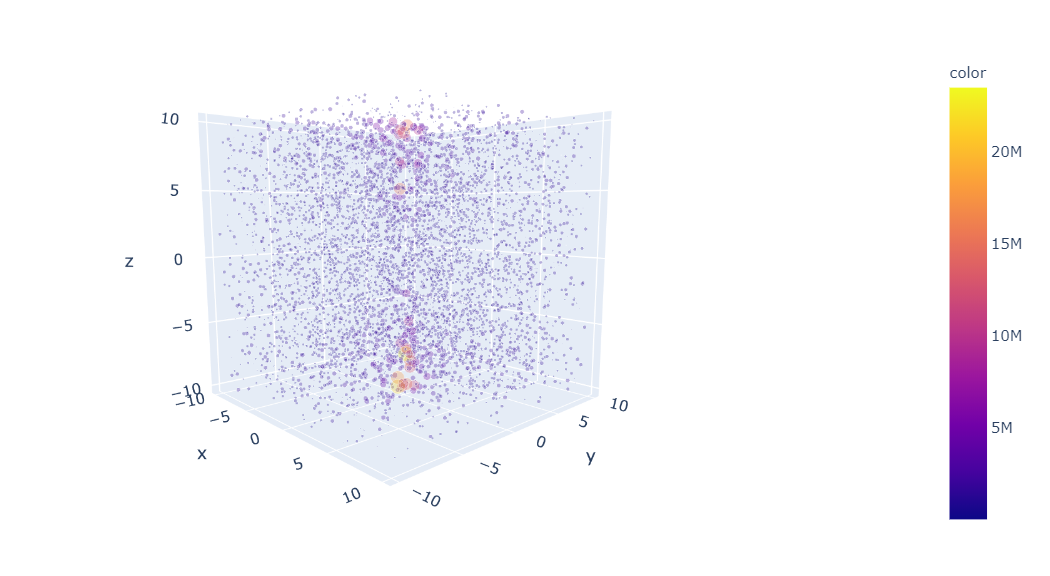
\includegraphics[width=0.5\columnwidth]{collab/Amp_Scatter.png}
      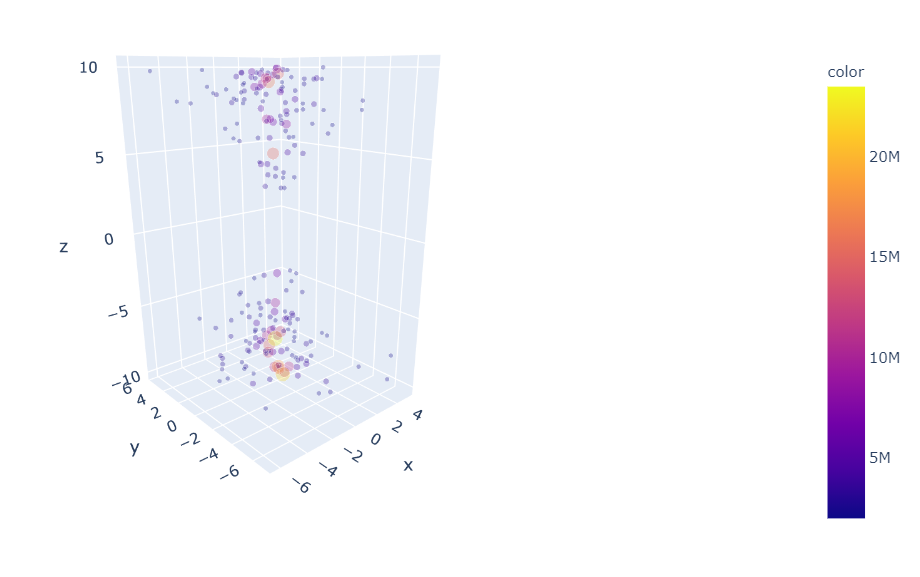
\includegraphics[width=0.45\columnwidth]{collab/Amp_Scatter_FoMthr_2e6.png}
      \caption{左右图均为 RMP 线圈和高 m 线圈进行协同优化后得到的 FoM 分布,marker 的大小和颜色表示 FoM 的大小,坐标轴 XYZ 轴分别为 RMP 线圈上下侧的 电流强度和高 m 线圈的电流强度。右图中过滤去除了 FoM 在 2e6 以下的点。}
\end{figure}

  线圈电流参数对 FoM 的影响参见上面几幅图,明显地有着 kAt 数较低 RMP 线圈和较高 kAt 数的高 m 线圈配合有可能产生较高的 FoM 的趋势。RMP 线圈相位及高 m 线圈旋转角度三者作为坐标轴后作类似上图,未发现明显变化趋势。


  高 m 线圈的电流幅度的增大会导致高 FoM 时 RMP 线圈的电流幅值容许范围得以增大。这告诉我们扰动场的大小要匹配(可以用磁通来衡量扰动场的大小)。


  


  


    
  
% \begin{itemize}
%     \item 对角度 $\varphi$ 这种有界参数,优化问题可以做一个扫描。但一旦引入了各扰动场的相对大小,优化方法可能就必需了。但 ERGOS 只适合串行,考虑将 ERGOS 中计算 Chirikov 径向分布计算等部分单独抽出来。FFT 可以不抽出来,因为线性性和平移性对每个线圈做一次计算就可以了。
% \end{itemize}


    
  

% 以下对三种扰动场仿真模拟细节陈述。


\chapter{扰动场作用下的热负荷分析}


% 在之前的研究中,研究者曾经用 GENRAY 相关代码将场线进行推测。

上一章中我们基于抑制 ELM 的需要提出了扰动场之间互相耦合的优化方法,这一章中我们进一步探究优化后的扰动场是否能够一定程度上缓解\Hmode 面对的热负荷问题。限于时间原因,以螺旋电流丝对热负荷分布的影响作为例子,探究外加扰动场控制热负荷的可能,可以调节材料受热的手段以材料损害。


如果粒子在刮削层中运动时不考虑场的横向方向上的输运,即不考虑碰撞的情况,则难以模拟打到偏滤器上的热负荷分布,粒子流分布非常集中。若是基于蒙特卡洛的思想,在粒子沿磁力线移动时引入横向漂移则可改善这一点。即粒子沿磁力线运动,但是每过一段满足指数分布的随机步长便发生横向漂移,使得粒子在不同磁力线之间可能发生漂移,在磁力线追踪程序的基础上添加了不确定性。
% 通过在一个边界磁面附近以均匀分布的种子为起点,计算打到偏滤器上各种负荷分布的计算。

\section{磁力线追踪与扩散}

  
磁力线追踪(\textit{F}ield \textit{L}ine \textit{T}racing, 磁力线追踪)是在磁场网格中进行插值和常微分方程求解得到真实磁场的磁力线分布的模拟手段。
磁力线追踪准备了插值和 ODE 的程序工具(Runge-Kutta 5 阶),可以产生迹线了(2D+3D),并且切换其他 ODE 数值计算方法相当方便。原有的 ERGOS 磁力线追踪似乎只能在磁面坐标系内进行 磁力线追踪,依据柱坐标进行重写之后可以在闭合磁面外追踪。


$$\dot{\vect{X}}(t) = \vect{B}(\vect{X}) $$

注意改变向量场的大小并不会改变上述常微分方程的轨迹,所以也可以有 $\dot{\vect{X}}(t) = \vect{B}/|\vect{B}| $,它仅改变到达轨迹上某点需要的时间。本论文中采用了 scipy 科学计算库中 integreate.ode 函数提供的龙格-库塔五阶方法,感兴趣的读者还可以在其提供的其他方法中进行选取。


当我们考虑粒子间的碰撞效应,粒子沿磁力线走过随机长度 $x$ 后发生一次横向漂移,

\begin{equation}
    p(x)=\frac{1}{\lambda} \exp \left(\frac{-x}{\lambda}\right),
\end{equation}

其中 $\lambda$ 为电子平均自由程。
横向漂移的方向在垂直于场的平面内随机均匀分布,而步长则在下面区间均匀随机分布,
\begin{equation}
  r \in[0, \sqrt{\frac{12 D_{\perp} \lambda}{v}}]
\end{equation}
其中 $D_{\perp}$ 为唯象的横向扩散系数而 $v$ 是电子速度。通过这种手段加入粒子扩散的因素可以一定程度上估计真实的热负荷分布。




% 尽管前一章节中对边界局域模的抑制是主要的评判扰动场的函数,评估热分布 $h(x,y)$ 优劣的函数,暂时选用梯度绝对值的 $\mathrm{L}^1$ 范数作为品质因子的计量标准,作为给定扰动场对应的热负荷分布的。
% \begin{equation}
%     \operatorname{FoM} =  \iint |\nabla h(x,y)| \mathrm{d} x \mathrm{d} y
% \end{equation}

\begin{figure}[htbp]
    \centering
    % \subcaptionbox{基于蒙特卡洛的磁力线扩散算法产生锯齿状的磁力线}{%
    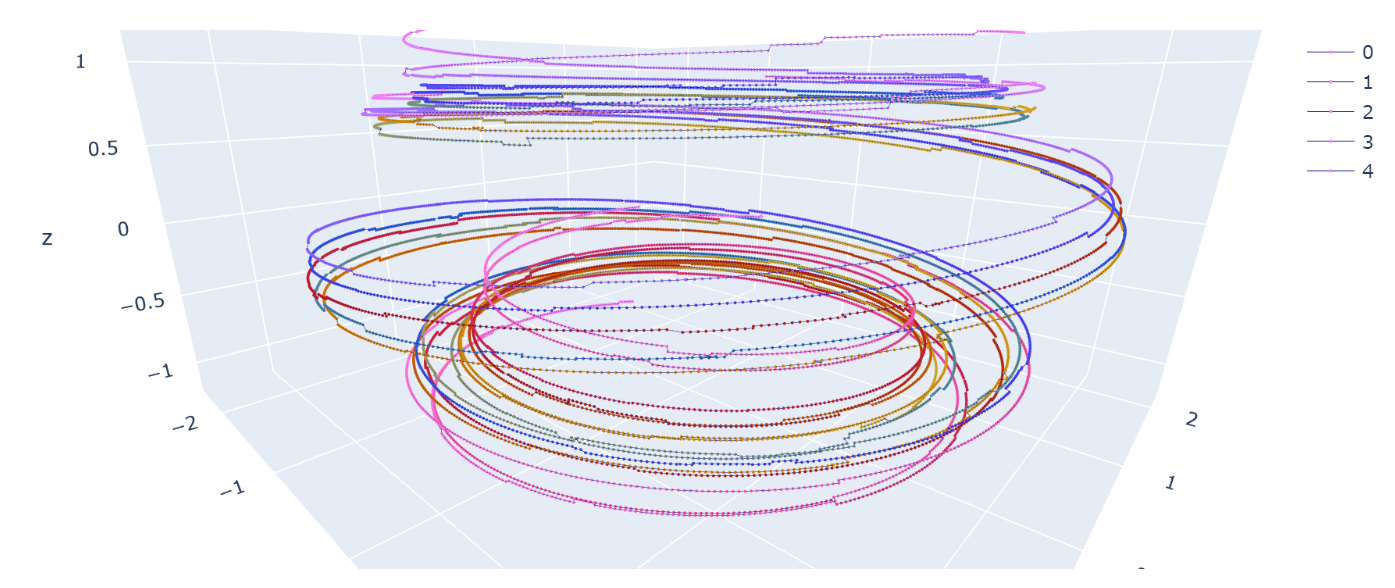
\includegraphics[width=0.80\columnwidth,keepaspectratio]{sawtooth_FLD.png}
    % }%
    \caption{基于蒙特卡洛的磁力线扩散算法产生锯齿状的磁力线}
\end{figure}


% The direction of the steps is uniform in the plane perpendicular to the field, while the step size $r$ is uniform in the interval:


该方法已在 Wendelstein 7-X 上成功应用以预估热负荷分布。

\section{螺旋电流丝作用下的热负荷分布}
我们在这一章中主要是通过磁力线的追踪和扩散技术来观察等离子体边界的磁拓扑变化,先从上偏滤器靶板附近邻域(由于该模拟位型是上单零位型)出发,射出磁力线,测量各磁力线长度和最深渗透 $s$,通过磁力线的长度我们可以判断其磁力线延伸后的簇状结构,即有哪些磁力线在追踪过程中仍是靠近的;通过最深渗透 $s$ 磁坐标半径可以判断能够射入等离子体最外闭合磁面内部的磁力线簇。如果热流和粒子流从等离子体中泵出的话,它们最有可能沿着能够深入等离子体的磁力线到其打击点上。

\subsection{原打击点附近的磁力线追踪模拟}
设置螺旋电流丝总电流大小设为 1.3 kAt,它引起了三维不对称的磁扰动结构,以 $n=1$ 主导,我们以它作为例子研究其引起的热负荷的分布的改变。
  
先在上偏滤器的一个邻域(环向联通)为起点进行磁力线追踪,对磁力线的延伸长度和最深渗透等离子体的 s,即径向半径进行直方图统计。

\begin{figure}[htbp]
  \centering
  
  \begin{subfigure}{0.4\textwidth}
    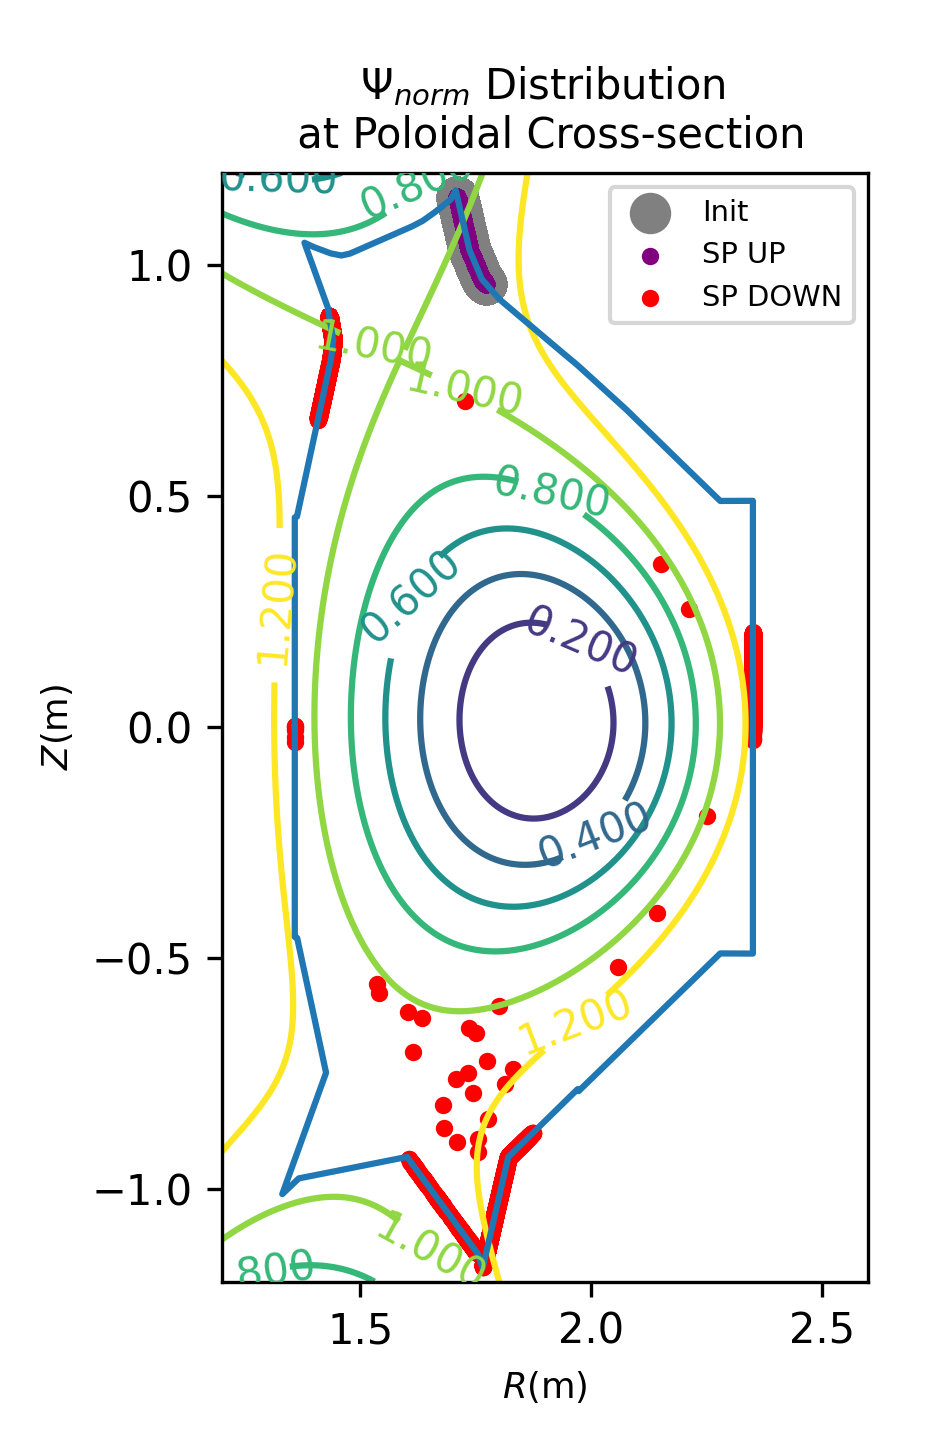
\includegraphics[width=0.9\columnwidth, keepaspectratio]{HCFs_EAST_73999/SP.png}
    \caption{磁力线追踪的起点,前后两个端点在极向切面上的分布,部分 磁力线追踪的计算到了时间限制停在了等离子体内。}
  \end{subfigure}%
  \begin{subfigure}{0.57\textwidth}
    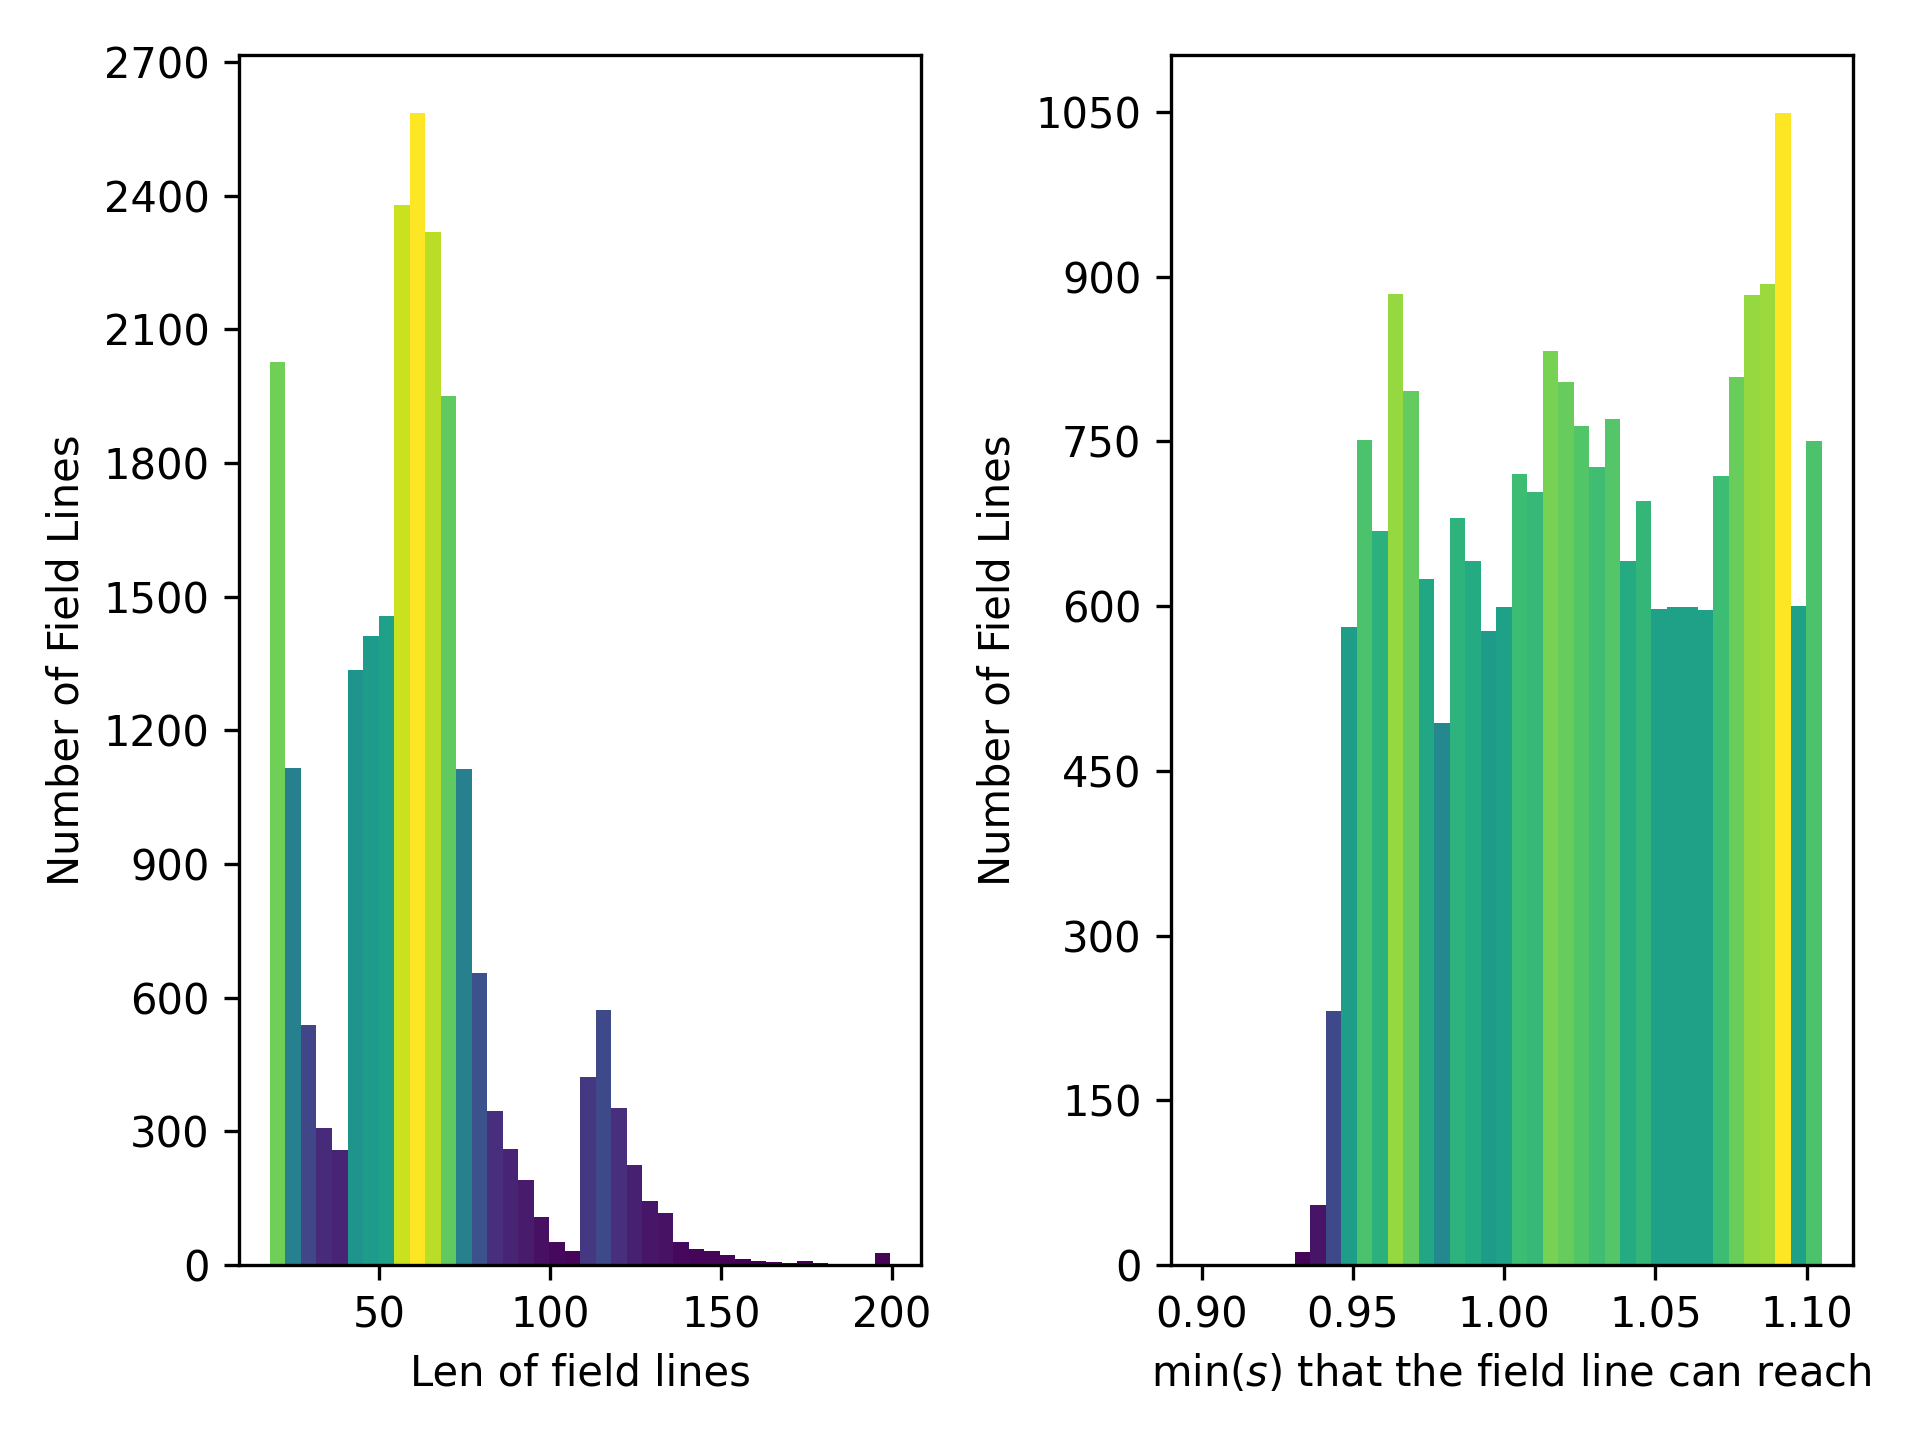
\includegraphics[width=1.0\columnwidth, keepaspectratio]{HCFs_EAST_73999/hist.png}
    \caption{磁力线追踪的长度和最深渗透 $s$ 分布的直方图}
  \end{subfigure}%
  \caption{上沿偏滤器靶板邻域作磁力线追踪的起点的模拟统计结果}
\end{figure}



可以观察到在螺旋电流丝的影响下,能够深入等离子体内部的磁力线追踪在图上出现了打击点分裂的特征,即原有的打击点处于偏滤器固定位置,通过螺旋电流丝引起了偏滤器靶板上打击点的带状分裂。$n=1$ 主导的螺旋电流丝扰动场影响下,其磁力线的扰动也有 $n=1$ 的特征。

\begin{figure}[htbp]
  \centering%
      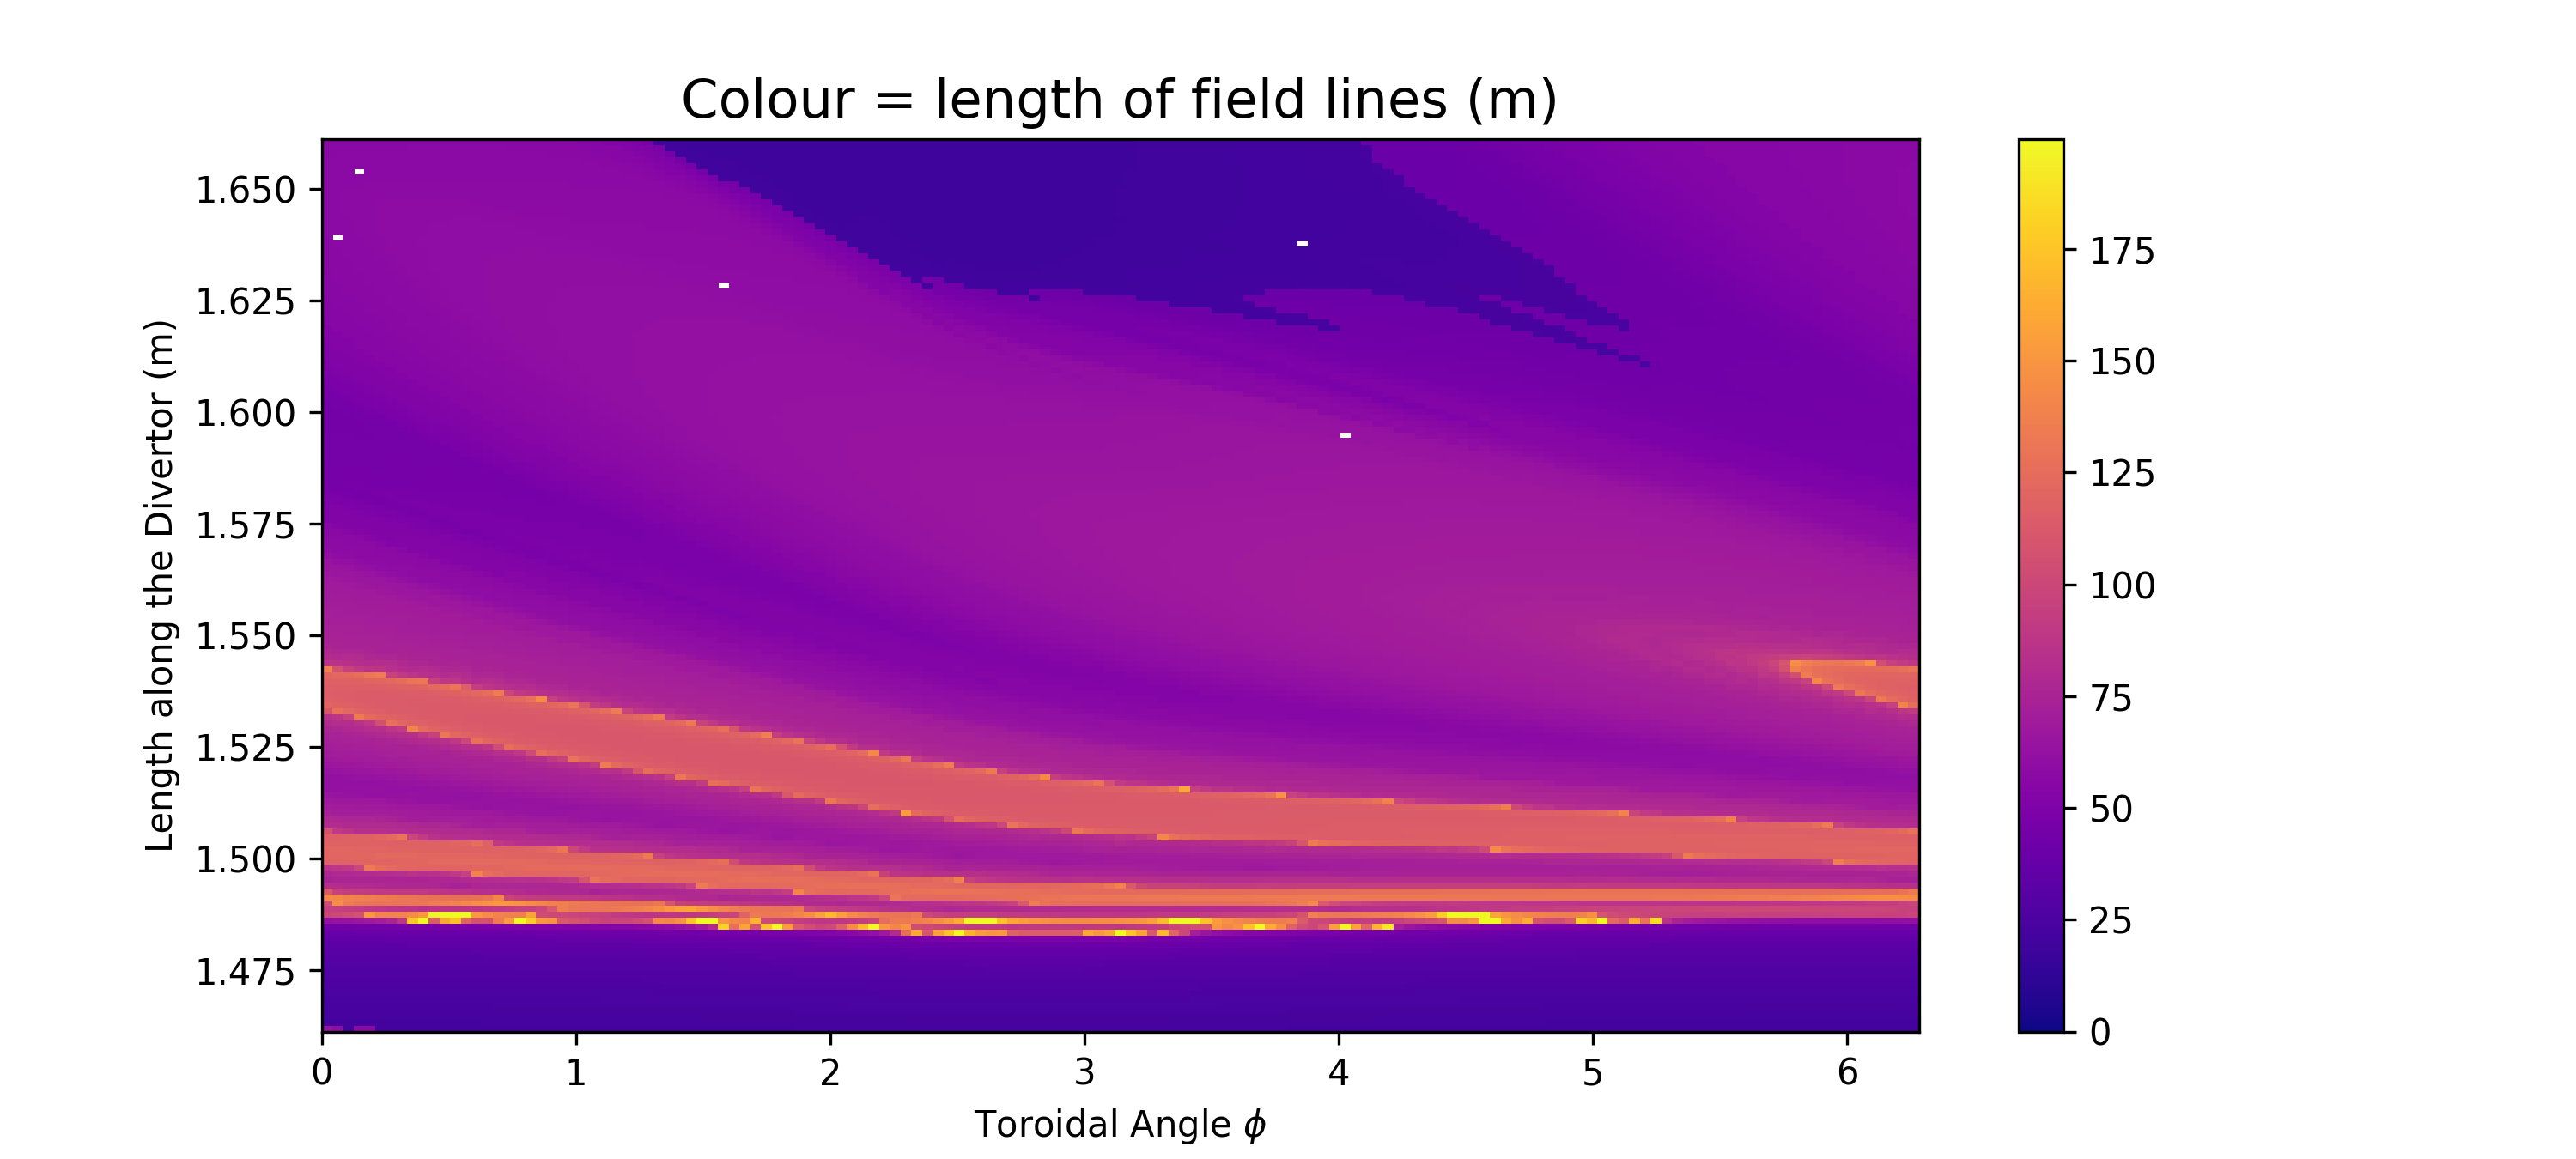
\includegraphics[width=1.0\columnwidth]{HCFs_EAST_73999/length_dist.png}
      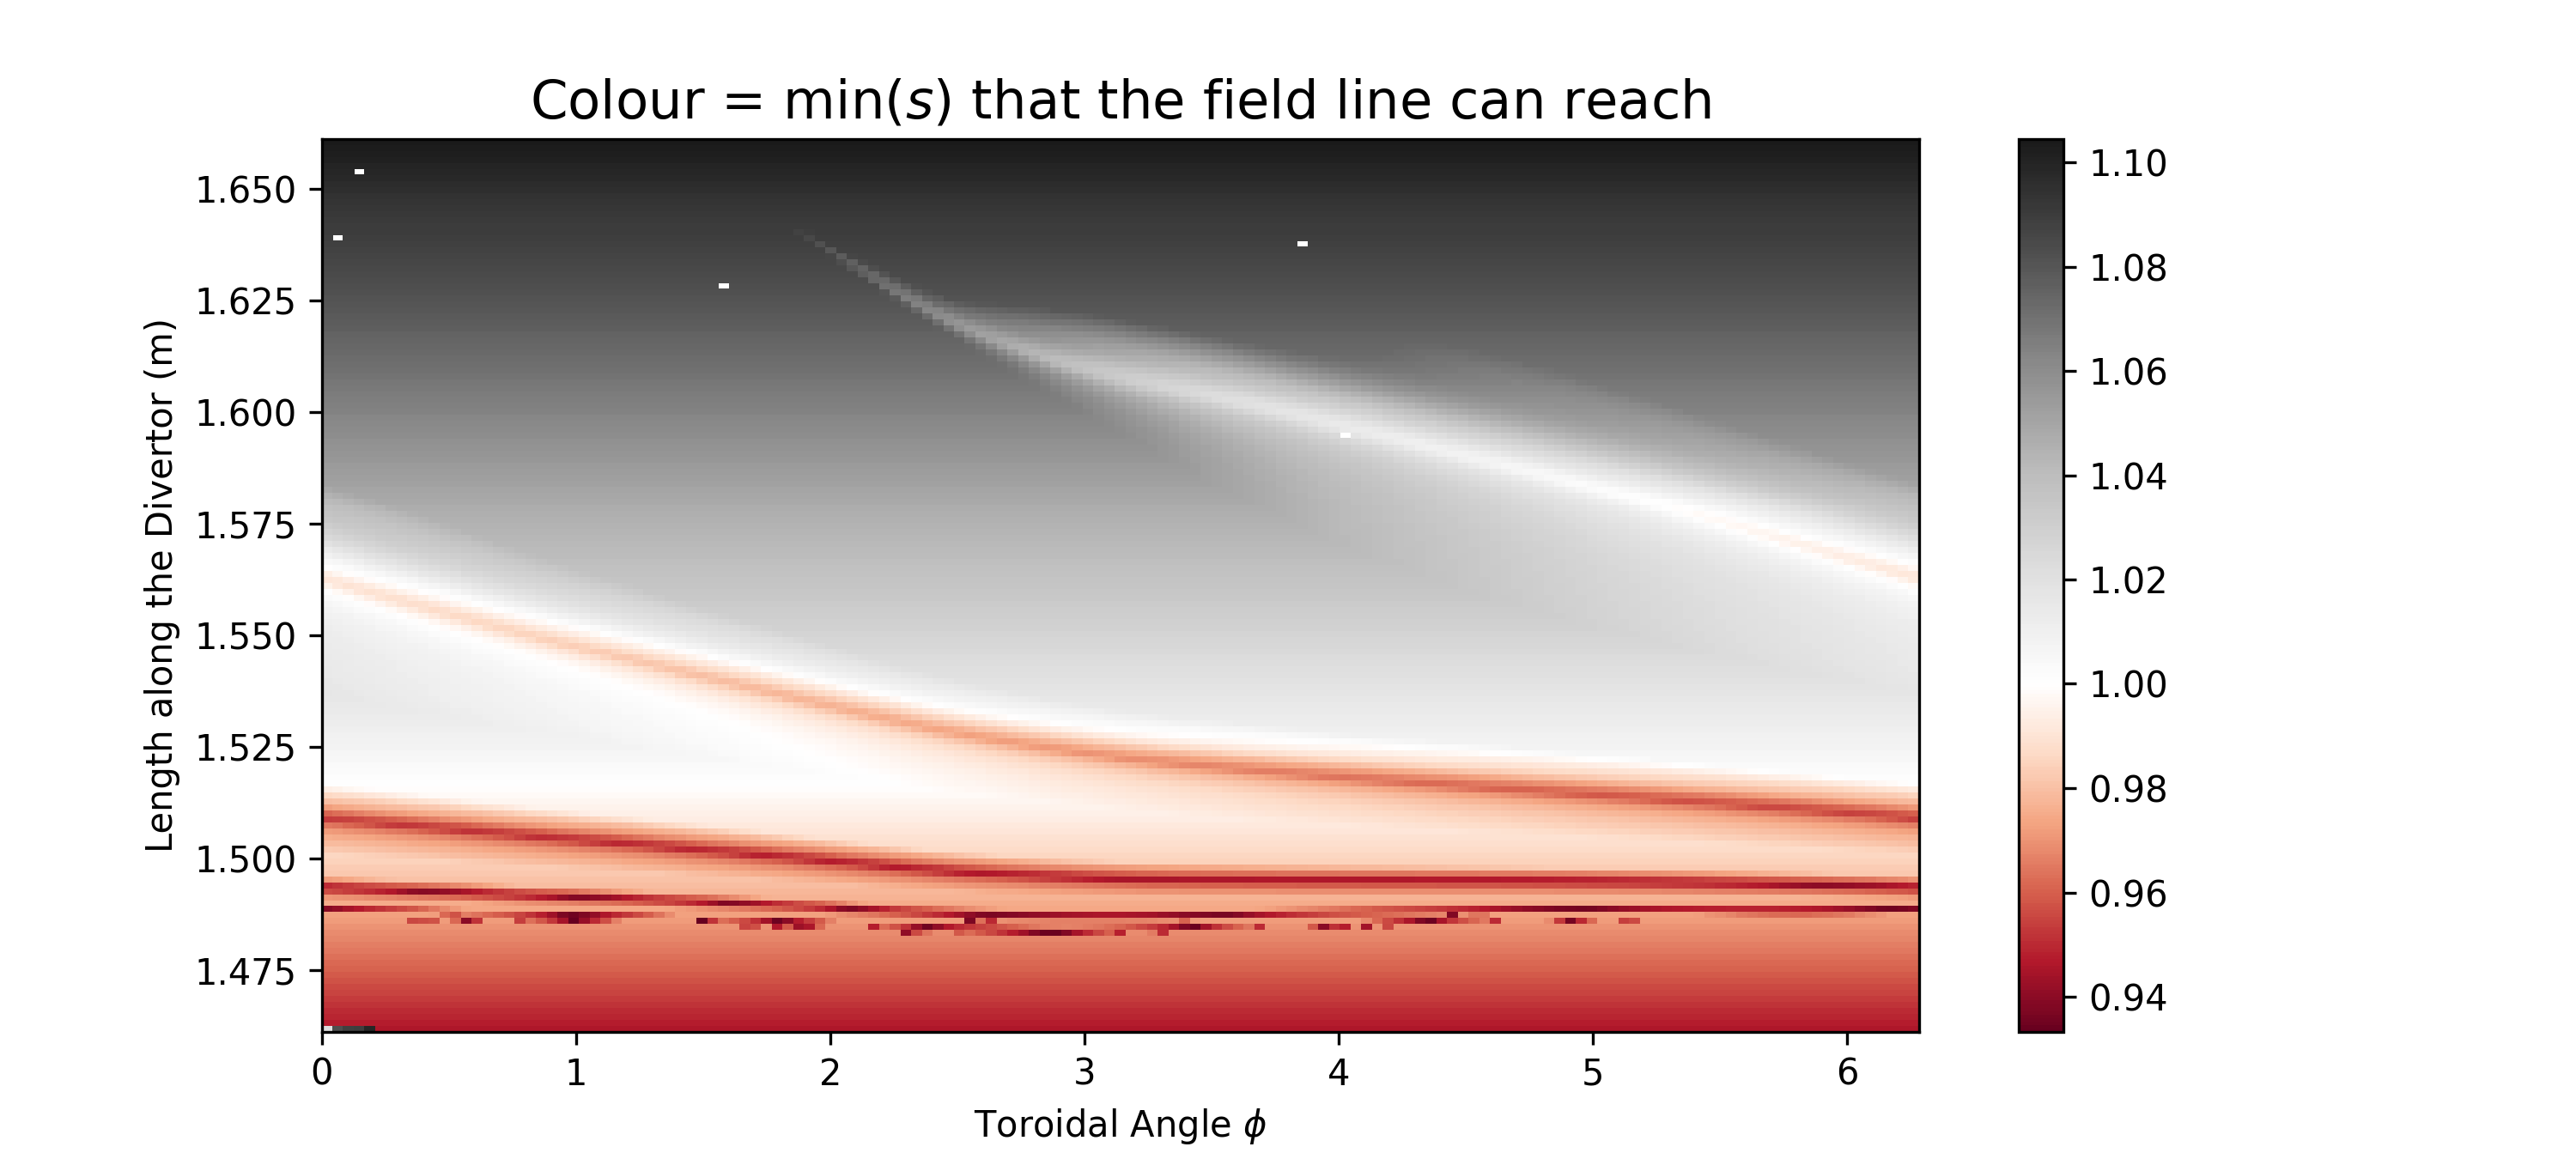
\includegraphics[width=1.0\columnwidth]{HCFs_EAST_73999/min_s.png}
      \caption{上下两图分别显示偏滤器上出发的磁力线的特征参数,上图显示的是磁力线长度,下图显示的是最深渗透 $s$。y 轴表示的是从偏滤器低场侧中心开始算起到磁力线追踪起点的距离。}
\end{figure}

\subsection{等离子体边界附近的磁力线扩散模拟}
现在等离子体边界外围布满磁力线追踪的起点,并且设为具有随机性的磁力线扩散,对其进行统计分析和到偏滤器上的打击点分布分析。 

\begin{figure}[htbp]
    \centering
  \begin{subfigure}{0.4\textwidth}
    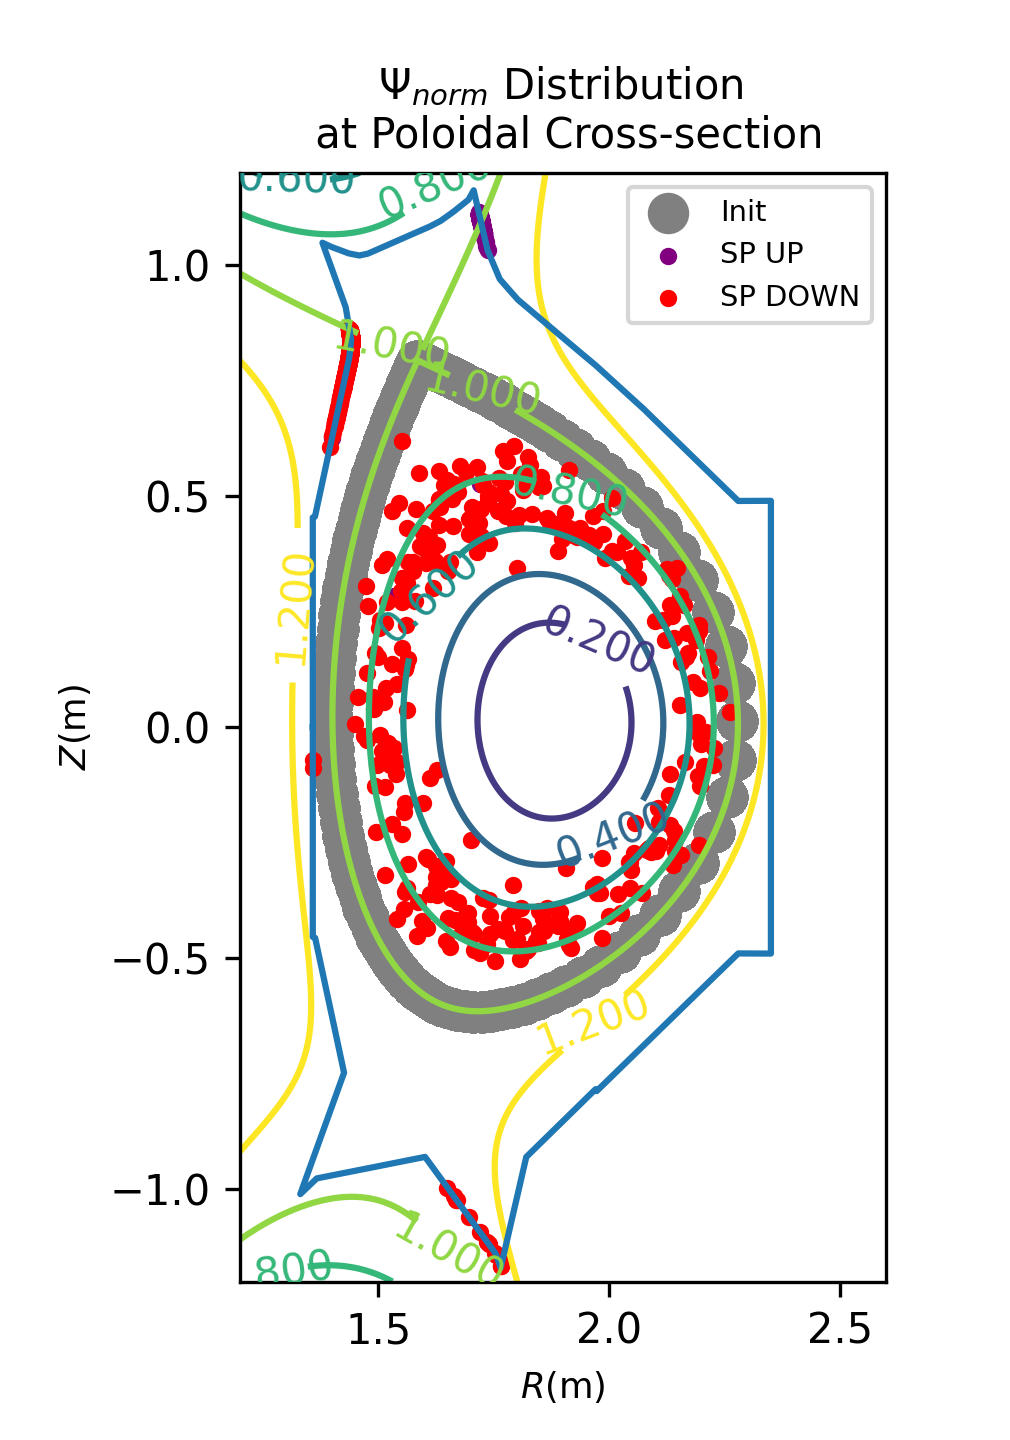
\includegraphics[width=0.9\columnwidth, keepaspectratio]{HCFs_EAST_73999_FLD/SP.png}
    \caption{磁力线追踪的起点,前后两个端点在极向切面上的分布,部分 磁力线追踪的计算到了时间限制停在了等离子体内。}
  \end{subfigure}%
  \begin{subfigure}{0.57\textwidth}
    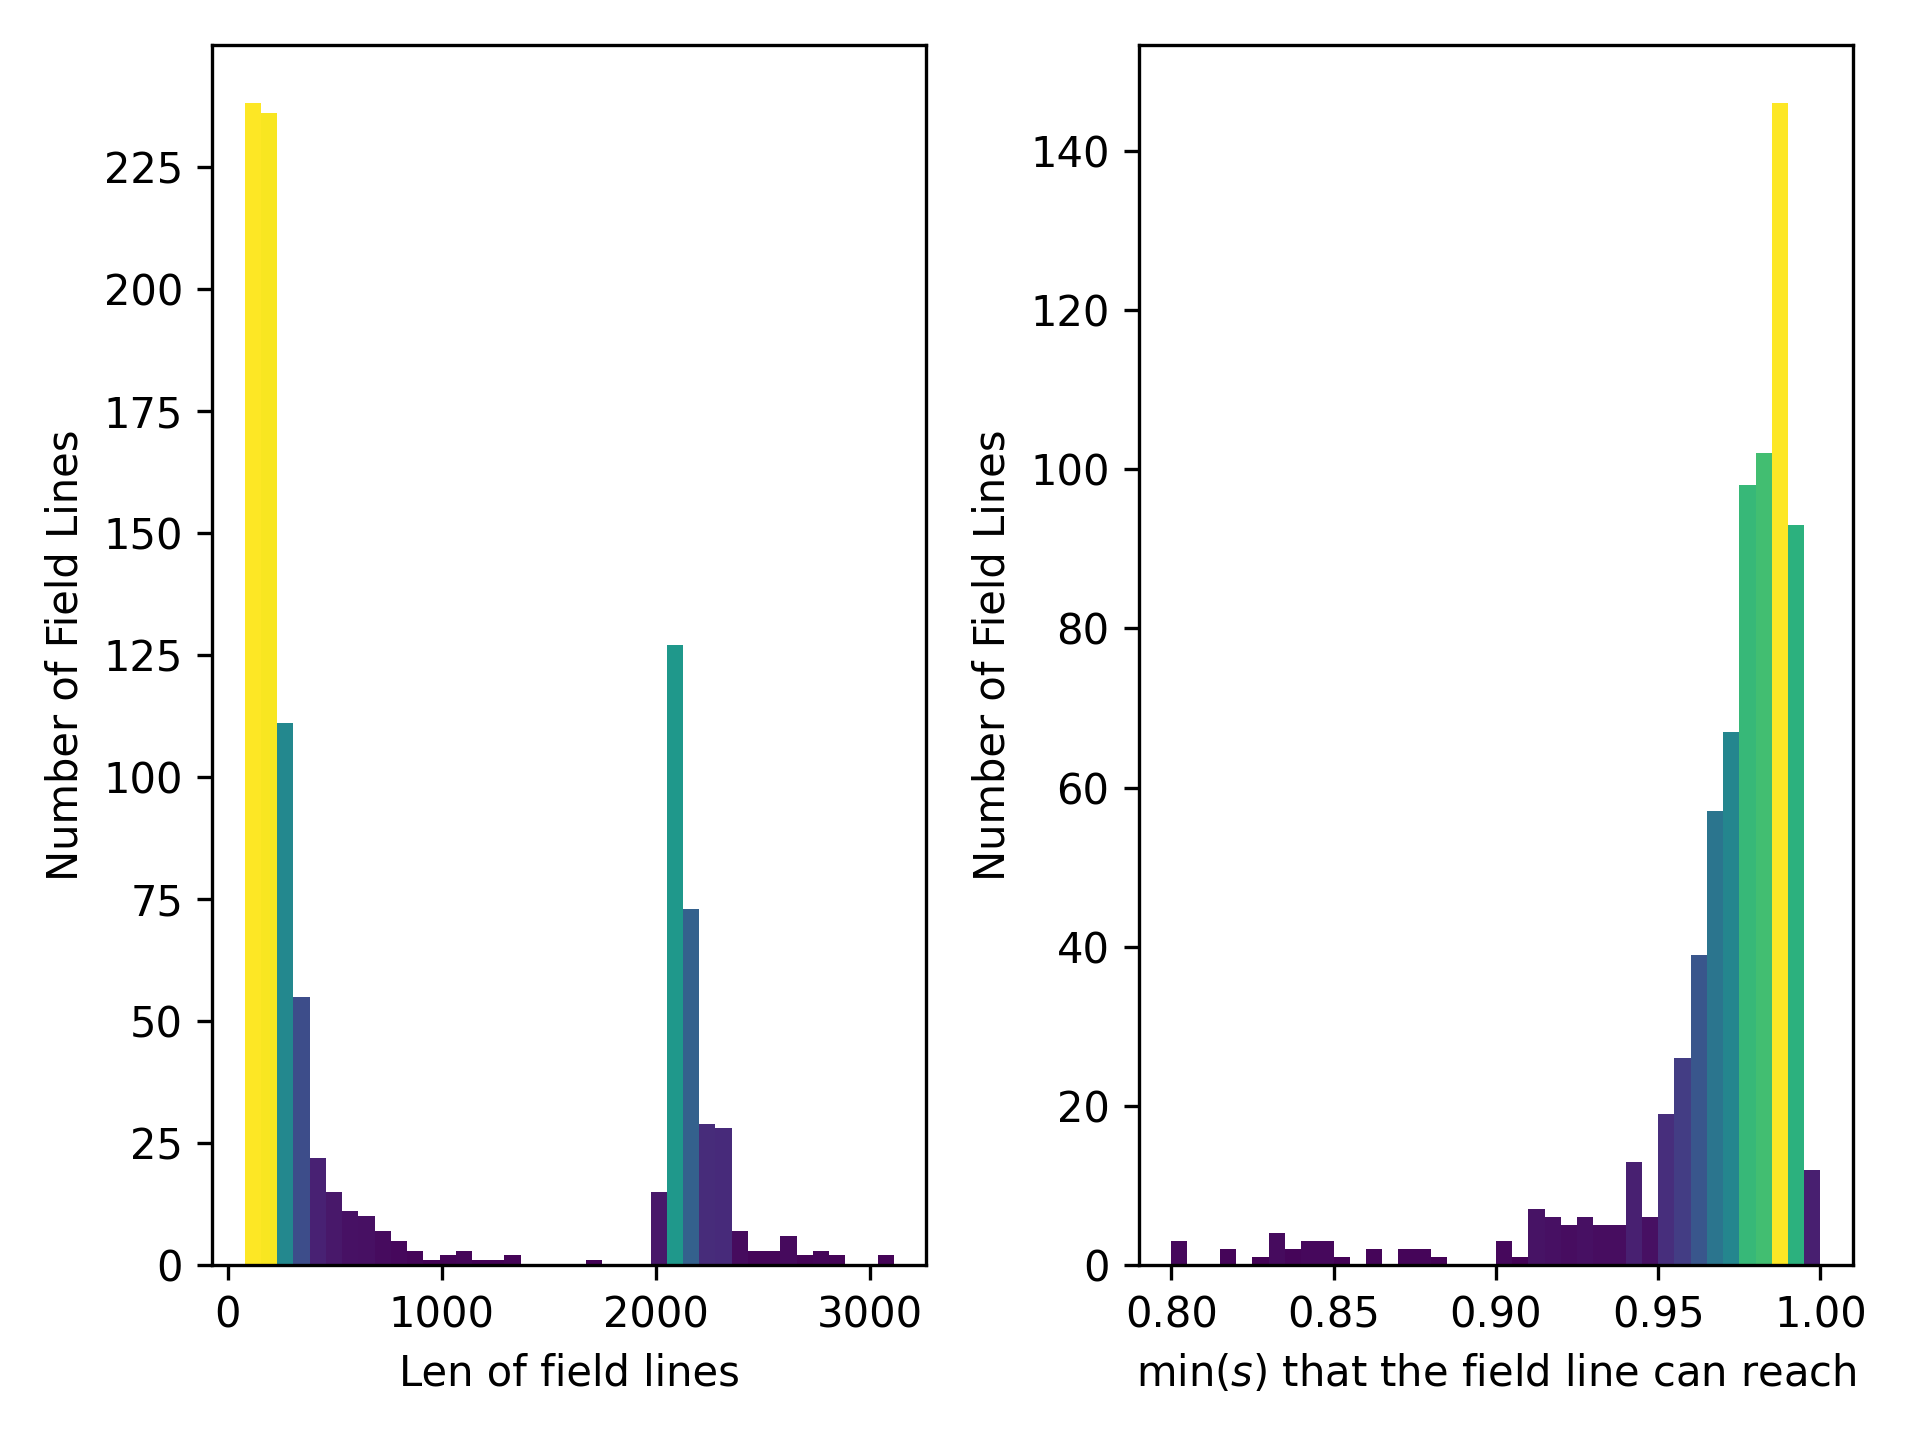
\includegraphics[width=1.0\columnwidth, keepaspectratio]{HCFs_EAST_73999_FLD/hist.png}
    \caption{磁力线追踪的长度和最深渗透 $s$ 分布的直方图}
  \end{subfigure}%
  \caption{以等离子体边界作磁力线追踪的起点的模拟统计结果}
  \end{figure}
  
通过对磁力线在原打击点周围的分布进行计数测量,一定程度上证实了扰动场引起的打击点的分裂,图 \ref{fig:sp-on-divertor}, 但数据量较少。
  
\begin{figure}[htbp]
    \centering%
        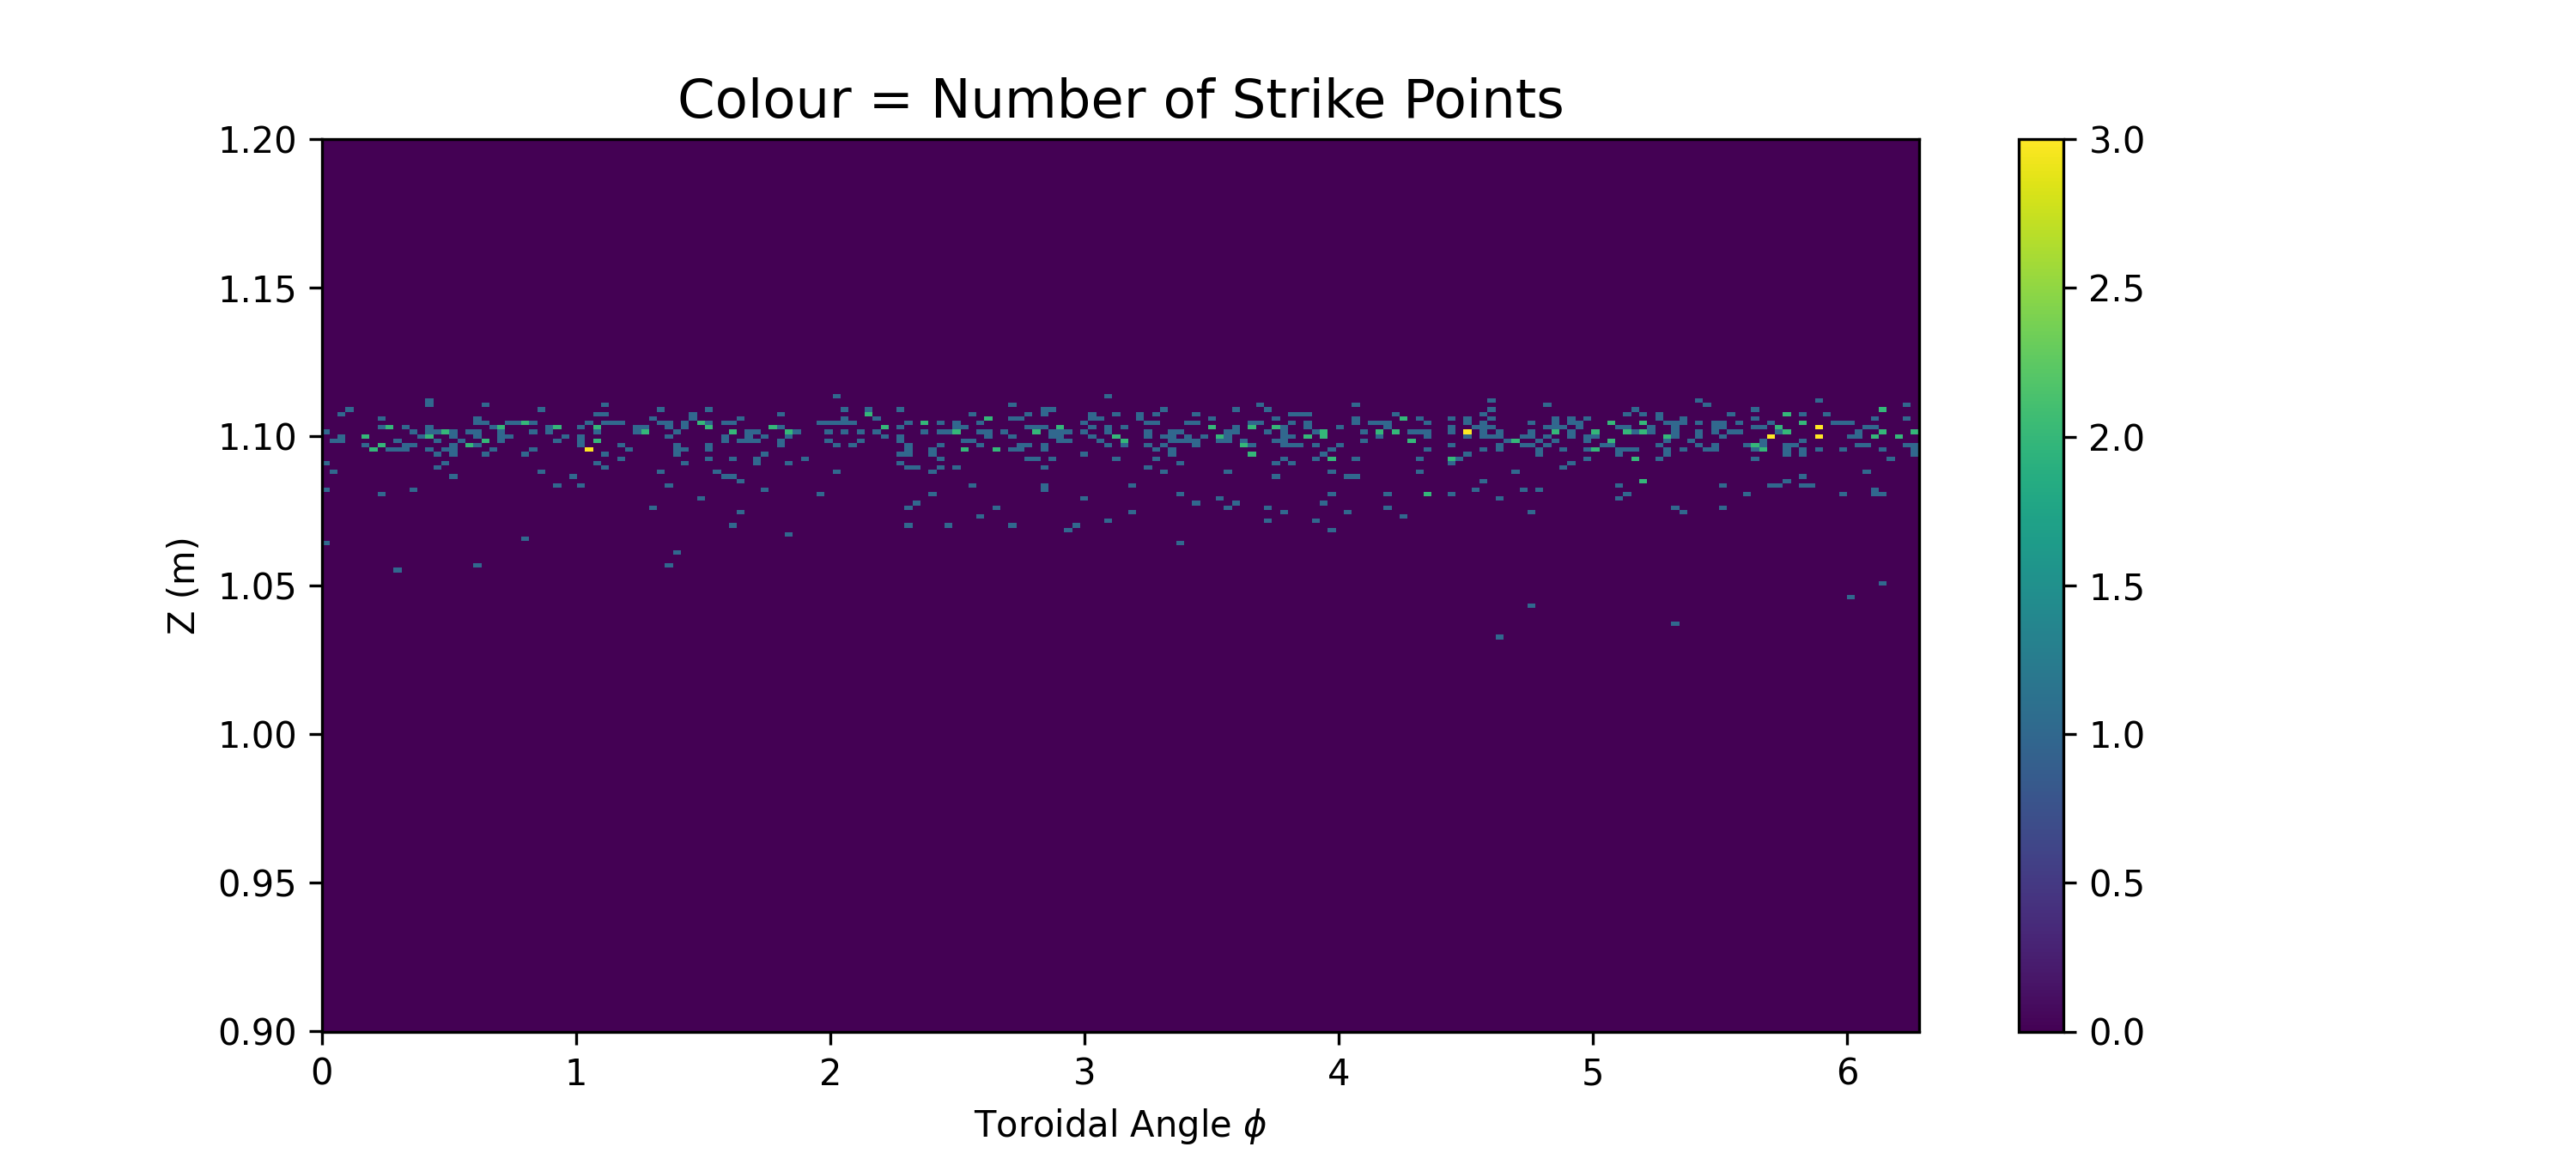
\includegraphics[width=0.70\columnwidth]{HCFs_EAST_73999_FLD/SP_dist.png}
        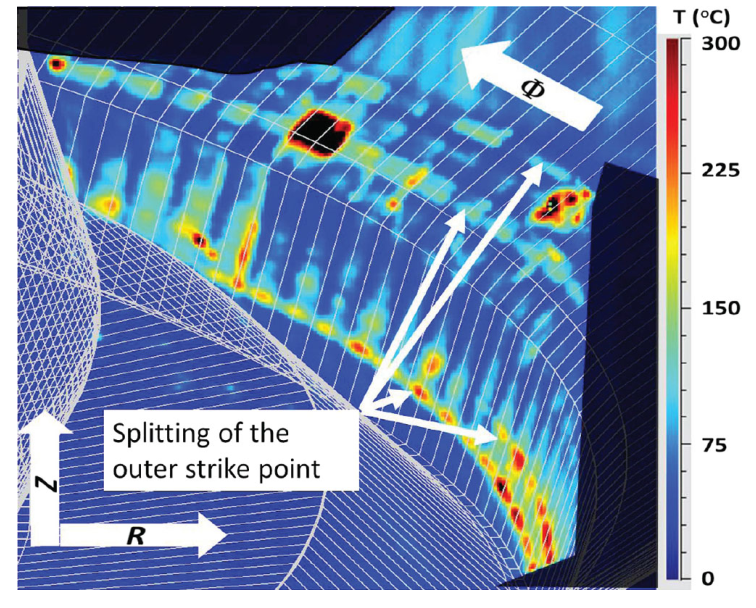
\includegraphics[width=0.29\columnwidth]{translate/liang_4.png}
        \caption{左图为等离子体边界上出发的磁力线扩散打到上偏滤器周围的能流密度(实际为二维直方图,计数为磁力线重点落在方格内的数目),右图为实际螺旋电流丝存在且为下单零位型时的下偏滤器旁温度分布,具体实验细节参见附录。}
        \label{fig:sp-on-divertor}
  \end{figure}

% 平衡场的磁力线追踪结果

% \begin{figure}[htbp]
%   \centering%
%       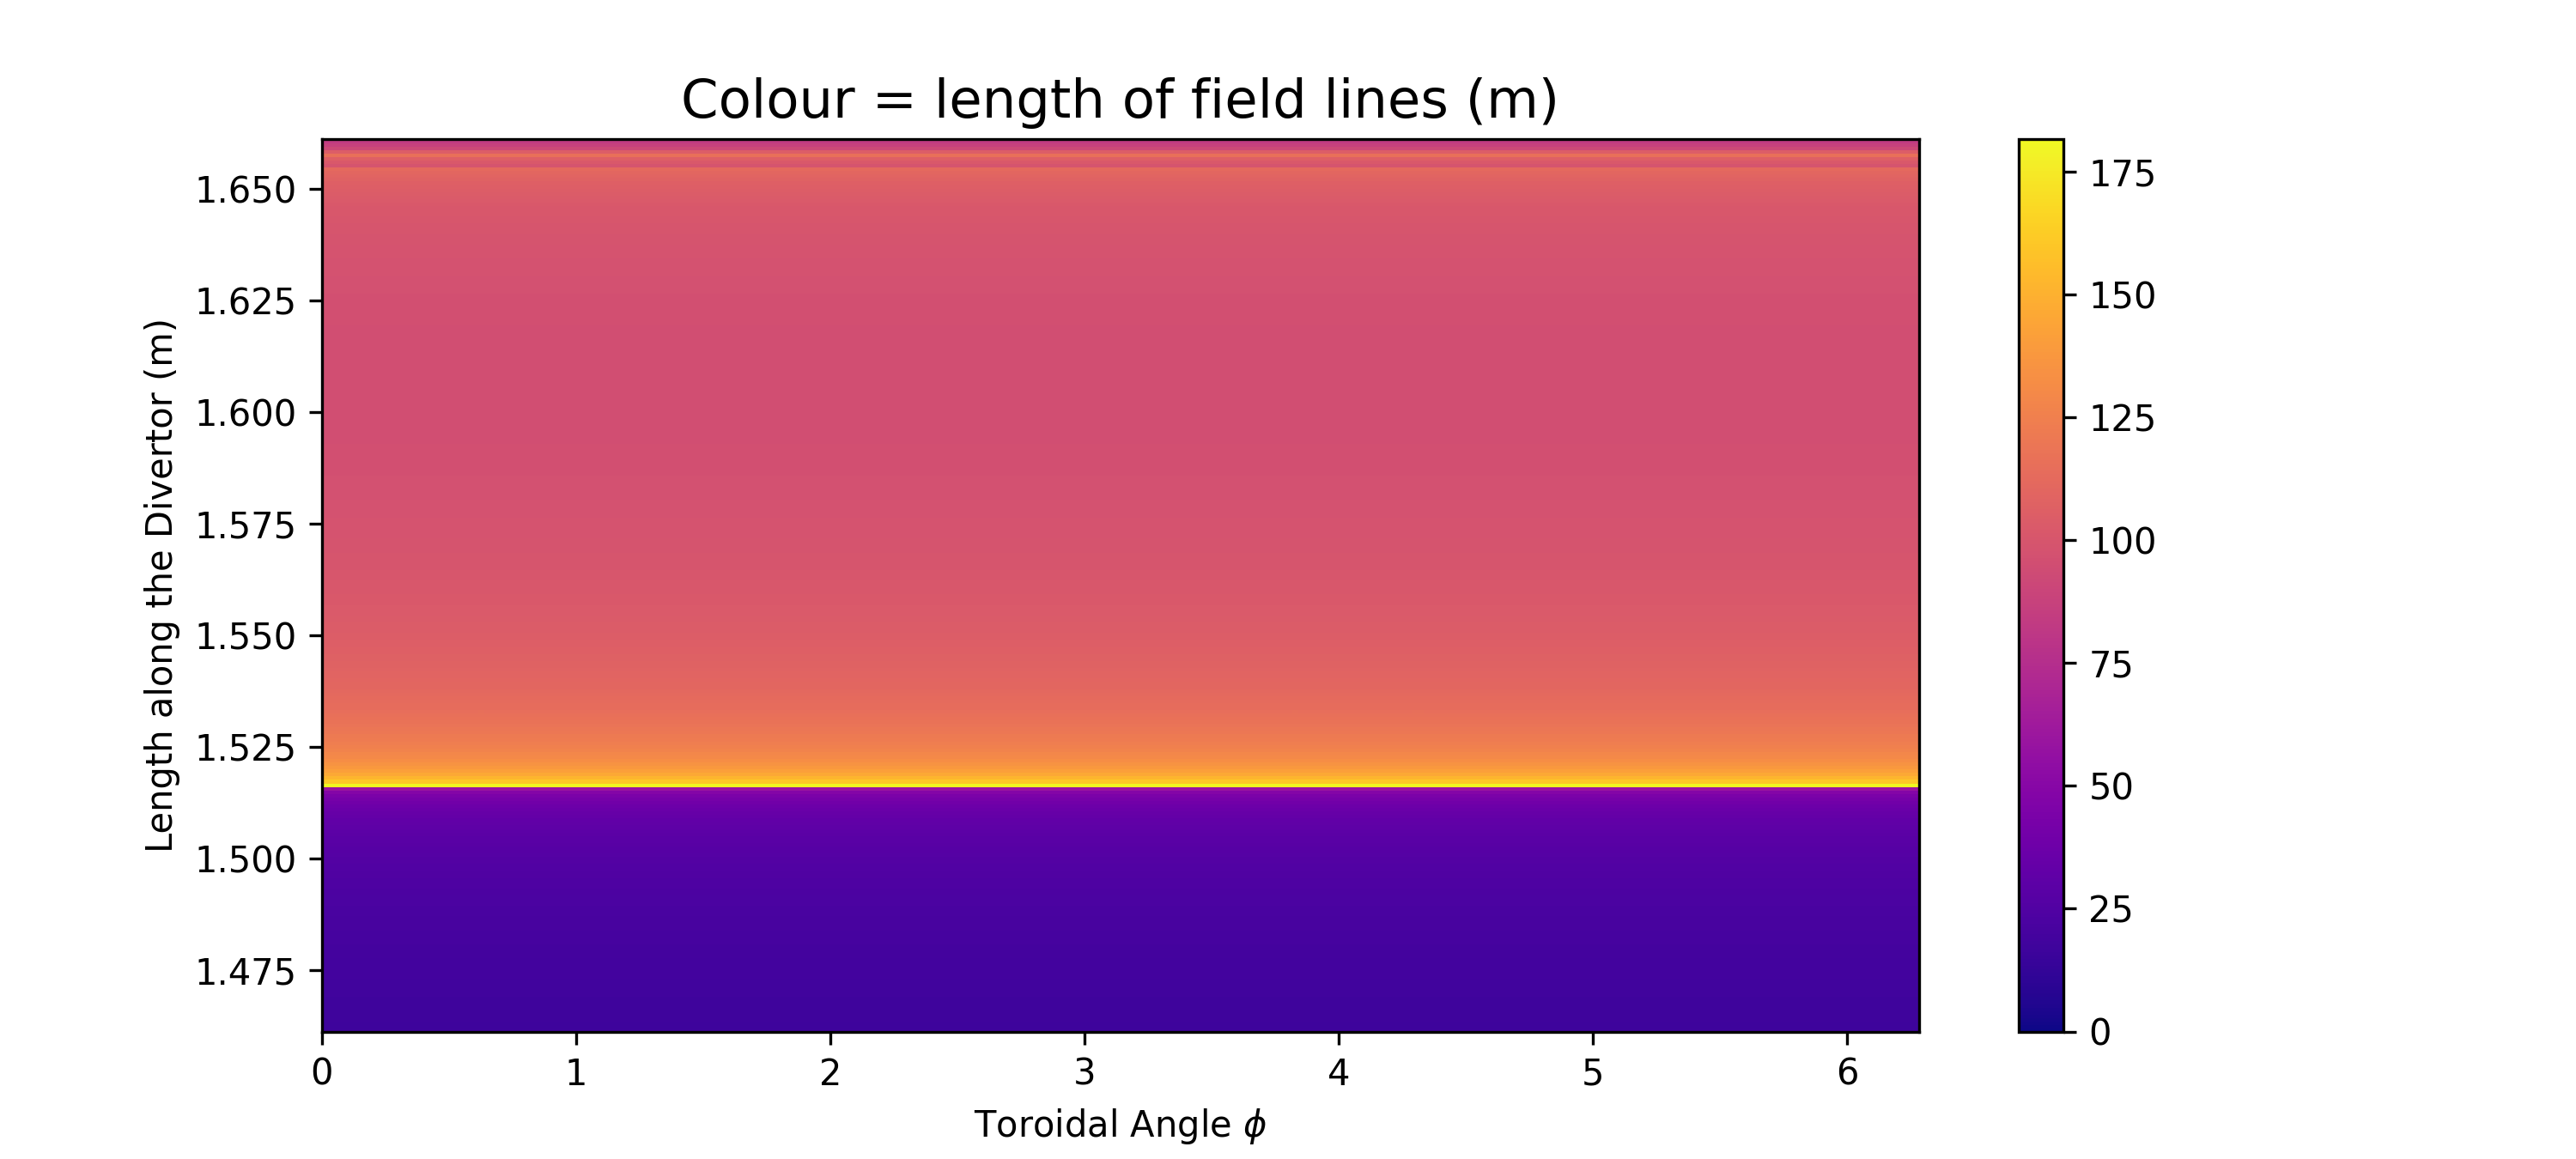
\includegraphics[width=1.0\columnwidth]{equili_EAST_73999/length_dist.png}
%       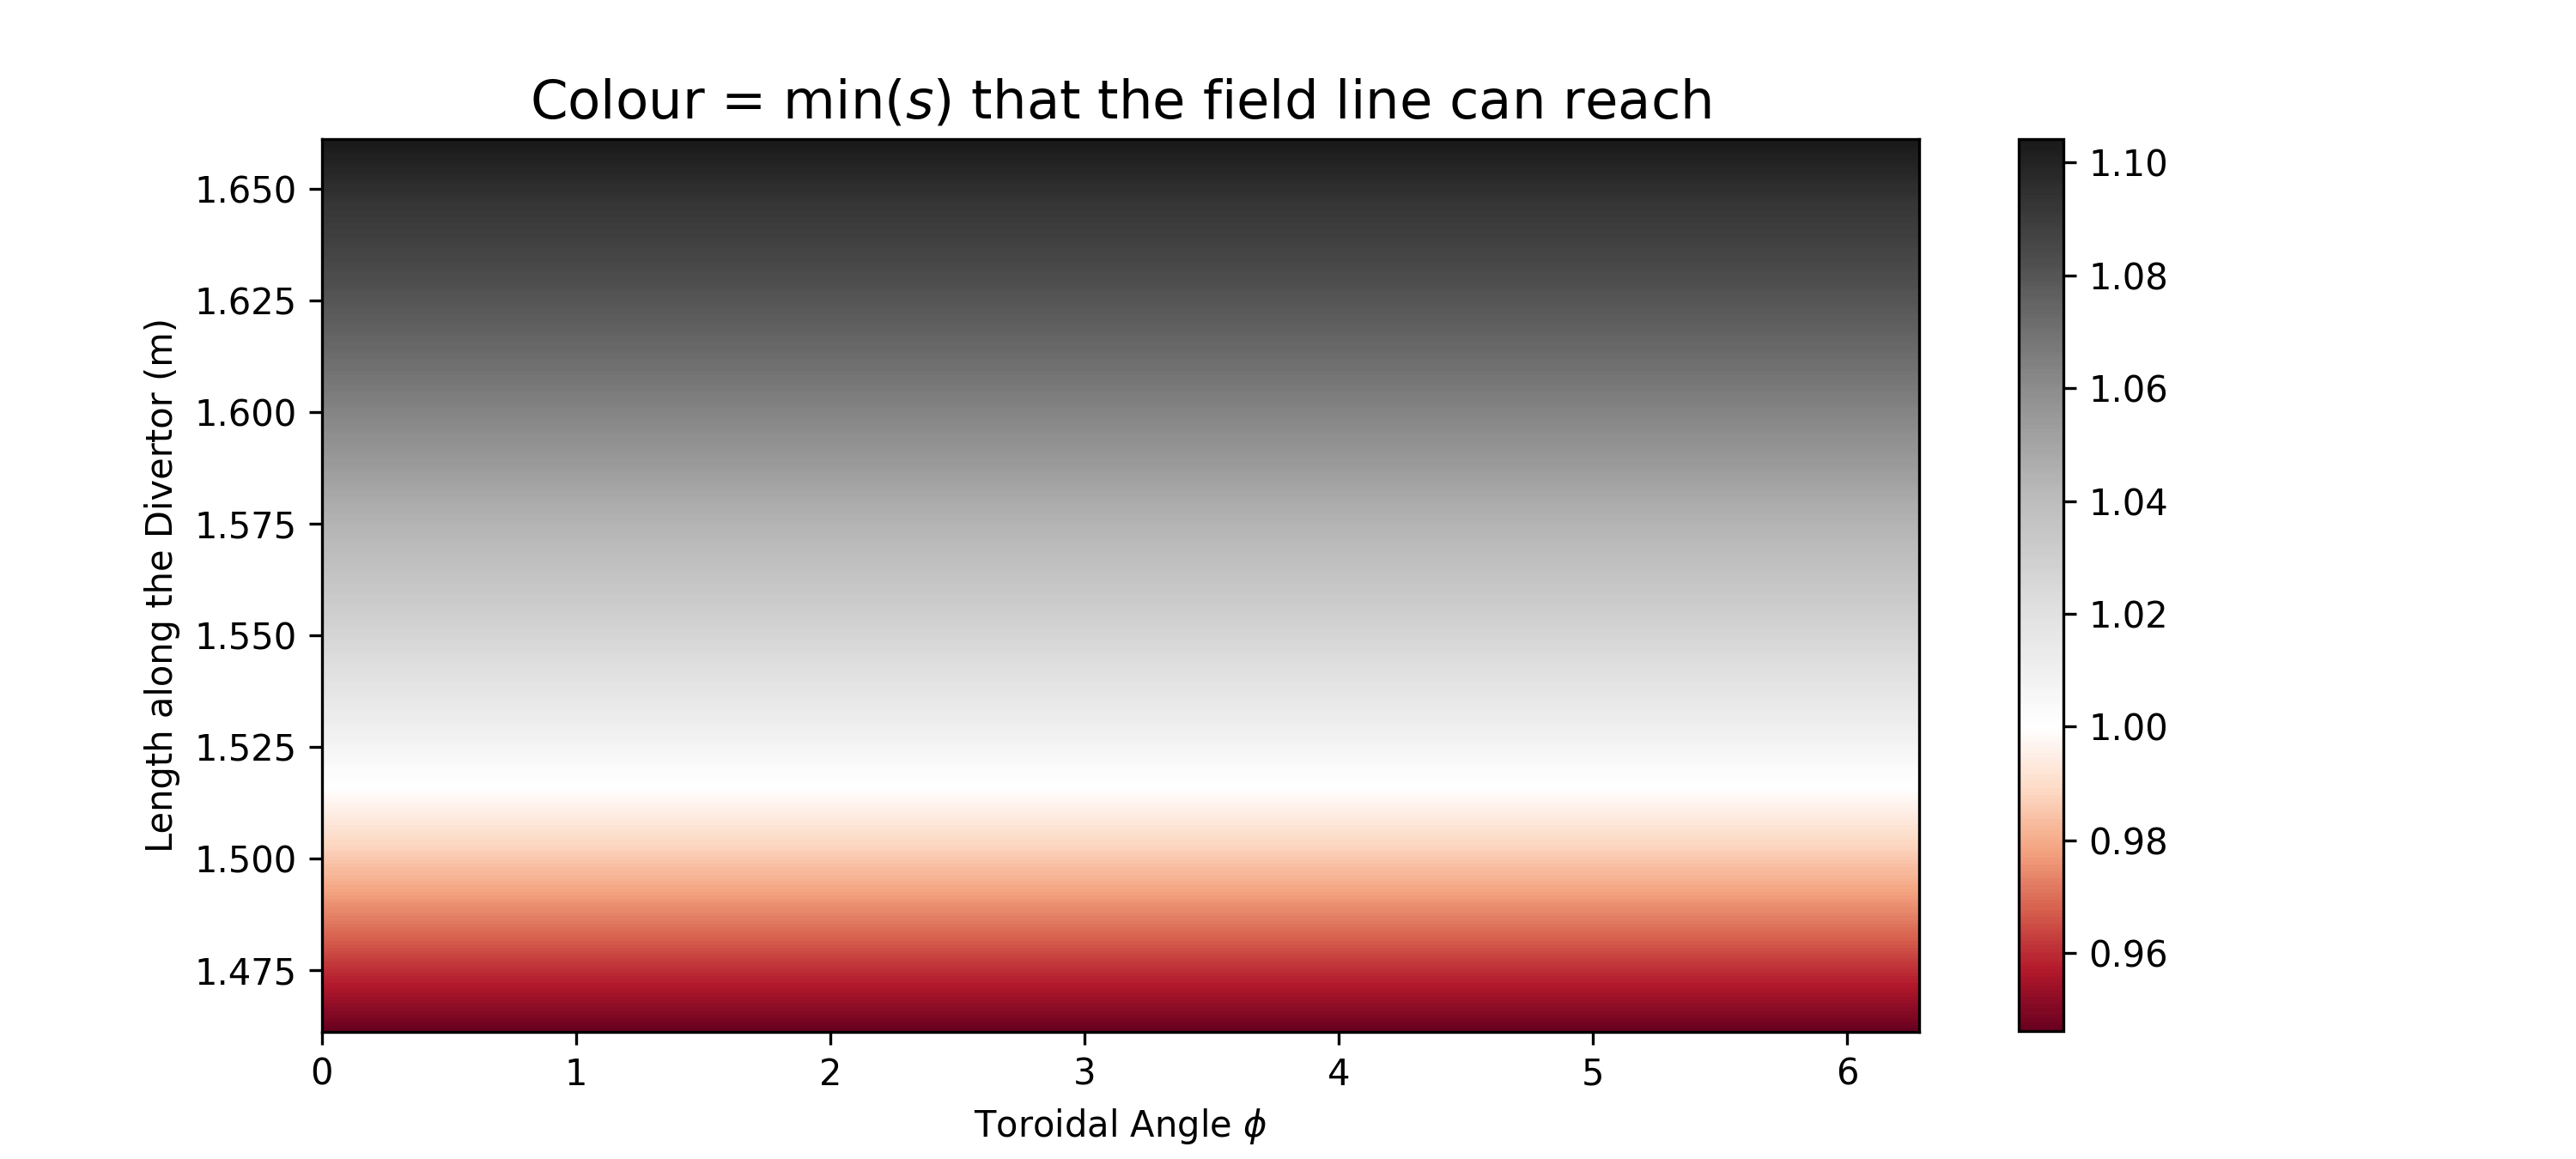
\includegraphics[width=1.0\columnwidth]{equili_EAST_73999/min_s.png}
%       \caption{平衡场的上偏滤器旁邻域内作起点进行 磁力线追踪,其最深渗透深度和长度分布。}
% \end{figure}


\section{小结}

本节通过基于蒙特卡洛思想的磁力线扩散模拟了可能的热负荷在偏滤器平板上的分布,未来该模拟结果可以与实验进行对比,验证热负荷估计的准确性。另一方面,这一结果初步揭示了通过非对称的扰动场,可以调节边界磁拓扑以调整粒子流及热负荷在偏滤器上的分布。

但仅仅如此还是不够的,如何对扰动场作用下偏滤器靶板上的磁力线落点位置进行归类总结,分析其形成的空间三维磁力线簇状结构是一个可以展开研究的重点内容。对这种有组织的三维结构的流场还需要细致的分析,不能单纯满足于算例的数值实验。
\chapter{随机场的湍流输运研究}

如果可以的话,我想从湍流输运的角度解释磁场边界拓扑对输运的影响。但我担心没有时间完成这一部分,Optional.

\chapter{总结}

在本毕设进行过程中几乎完全重构了一遍 ERGOS 程序,使得磁谱分析的工具变得尤其方便使用,从目前的扰动场的模拟结果我们可以看出,螺旋电流丝产生的及其强烈的共振分量有着很强的激发磁拓扑边界随机层的能力。高 m 线圈、低 n 线圈(RMP 线圈)远没有其作用强烈,为了使其磁通适配,需要适当地增加高 $m$ 线圈和 RMP 线圈的电流大小。

\section{单一扰动场}
对 RMP 线圈(低 $n$ 线圈)的研究发现
\section{扰动场协同}
\section{对实验参数的优化指导}

\section{展望}
\begin{enumerate}
    \item 考虑等离子体反馈后会提高有理面产生磁岛所需要的径向扰动共振分量强度,
    未来通过随机场的湍流输运研究可以对它有更深刻的认识。
\end{enumerate}


\subsection{有限体积法}
在有限体积法进行计算的过程中,我们所储存的变量值是偏微分返程中守恒量在网格中的平均值。与之类似但有些不同的是,在有限元法中,我们用试函数使得所计算得到的函数是函数空间中最优的函数。

\subsubsection{双流体模型}
将等离子体视为离子和电子相互渗透的双流体来看待,分别视为服从麦克斯韦分布的等离子体,相比于单流体的模型更能反映出电子和离子的不同响应特性和各自的流体特征。

各种扰动场对 ELM 的发生起到了显著的控制作用,而在扰动场施加时等离子体边界浮现的随机场则对粒子和热输运均影响深远。这一部分的研究设计将模拟中加入**。从湍流输运的角度解释磁场边界拓扑对输运的影响可能有较好的效果。


\subsection{有限元、有限体积法}
偏微分方程的求解问题构成了现代工程领域许多重要的设计工作,计算框架和数值理论在各种高性能计算处理器的基础上的组合计算成为了现代工业设计的重要设计及优化工作。

有限元法(Finite Element Method, FEM)在多物理场分析中很成功,一方面它非常通用,另一方面有限元可以对不同计算域内物理问题适合的算法进行组合,这对于多物理问题而言是一个关键优势。

尽管有限元可以自然地处理弯曲和不规则几何图形,但有限元背后的数学相对有限体积法(Finite Volume Method, FVM)更复杂一些。有限体积法中自然地对物理偏微分方程组中的守恒量进行在网格上进行积分,离散值表示的是单元内该守恒量的积分平均值。于是有限体积法的重点在于如何通过单元(cell)的积分平均值插值表示单元边界的守恒量流量,即流函数。

% 最后,对于时域时间上的仿真,为了效率往往需要使用显式求解器。但是有限元在实施此类技术方面存在困难,因此建议不要使用它。

\begin{itemize}
    \item EMC3-EIRENE
    \item \textit{FEniCS\footnote{\url{https://fenicsproject.org/}}} 是开源(LGPLv3)的偏微分方程计算框架。 FEniCS 中丰富的 Python-C++ 接口使得科学工作者可以迅速地将他们面对的科学模型转化为有限元程序逻辑。在这里我们选取 FEniCS 是因为其后端的 PETSc\footnote{\url{https://www.mcs.anl.gov/petsc/}} 在支持 OpenMP、OpenCL 和 CUDA,在针对 PDE 的硬件优化上几乎无出其右,可以在几乎在任何并行计算硬件平台上得到快速应用。\underline{考虑到毕设时间的有限并且可能将考虑非线性等离子体响应},具备高层接口的 FEniCS 是快速实现偏微分方程的手段\inlinecite{FEniCS_LangtangenLogg2017}。
    \item \textit{SU2\footnote{\url{https://su2code.github.io}}} 工具箱是基于 C++ 偏微分方程的求解分析工具并可以在给定条件基础上进行设计优化。这套工具是为计算流体力学和空气动力学形状优化而设计的,但它也能够进行扩展来处理任意几何的控制方程,例如位势流,弹性问题,电流力学问题,化学反应流以及其他问题。
    \item \textit{MFEM\footnote{\url{https://mfem.org/}}} 与 FEniCS 类似,MFEM 也支持对后端采用 PETSc 进行并行加速。其在电磁场领域有过一些研究,在本论文中被采用作为辅助验证工具。
    \item \textit{\mdddc \footnote{\url{https://w3.pppl.gov/~nferraro/m3dc1.html}}} 由美国普林斯顿大学等离子体实验室开发,是一个聚变等离子体界影响深远的非线性双流体模拟计算工具。但由于中美关系恶化及其代码闭源问题,\mdddc 的数值高精度算法及各类成果在本论文中仅作为数值理论的参考。
\end{itemize}


环向低速转动的低 n 扰动场已经在 J-TEXT 等实验中应用,FEniCS 实现 toy 级别的应用
    
One day in 100+ lines.

\begin{equation}
  \nabla \times\vect{H} = \vect{j}+\frac{\partial \vect{D}}{\partial t} 
\end{equation}

Forward Euler
\begin{equation}
  \int \vect{B}^{n+1}\cdot\vect{B}^* dx =\int \vect{B}^n\cdot \vect{B}^* - \Delta t  \nabla\times\vect{E}^n\cdot\vect{B}^* dx
\end{equation}

TODO:
\begin{enumerate}
  \item 和 ERGOS 静磁学毕奥萨伐尔定律进行单一线圈精度对比。
  \item 比置零更精确的边界条件(PML 或其他吸收层边界)引入。
  \item Maxwell 方程高阶算法和混合元(电磁场错开)的引入。
\end{enumerate}




\begin{figure}[t]
\centering
\subcaptionbox{二维铁包层内外极向均匀分布的异向电流丝产生的磁场分布}{%
    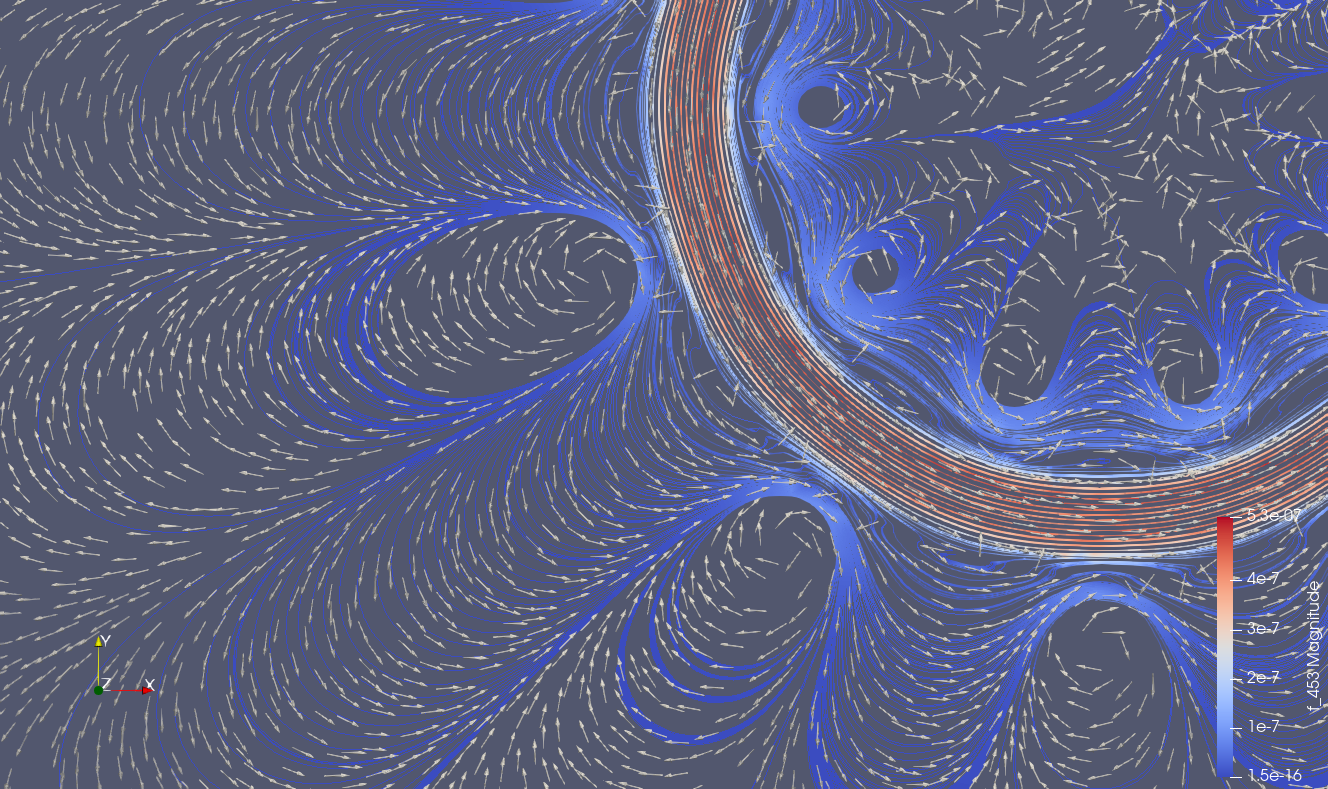
\includegraphics[width=0.45\columnwidth,keepaspectratio]{fenics/test/fenics_electrostatic_case.png}
}\hfill
\subcaptionbox{环形线圈产生的磁场分布示意图}{%
    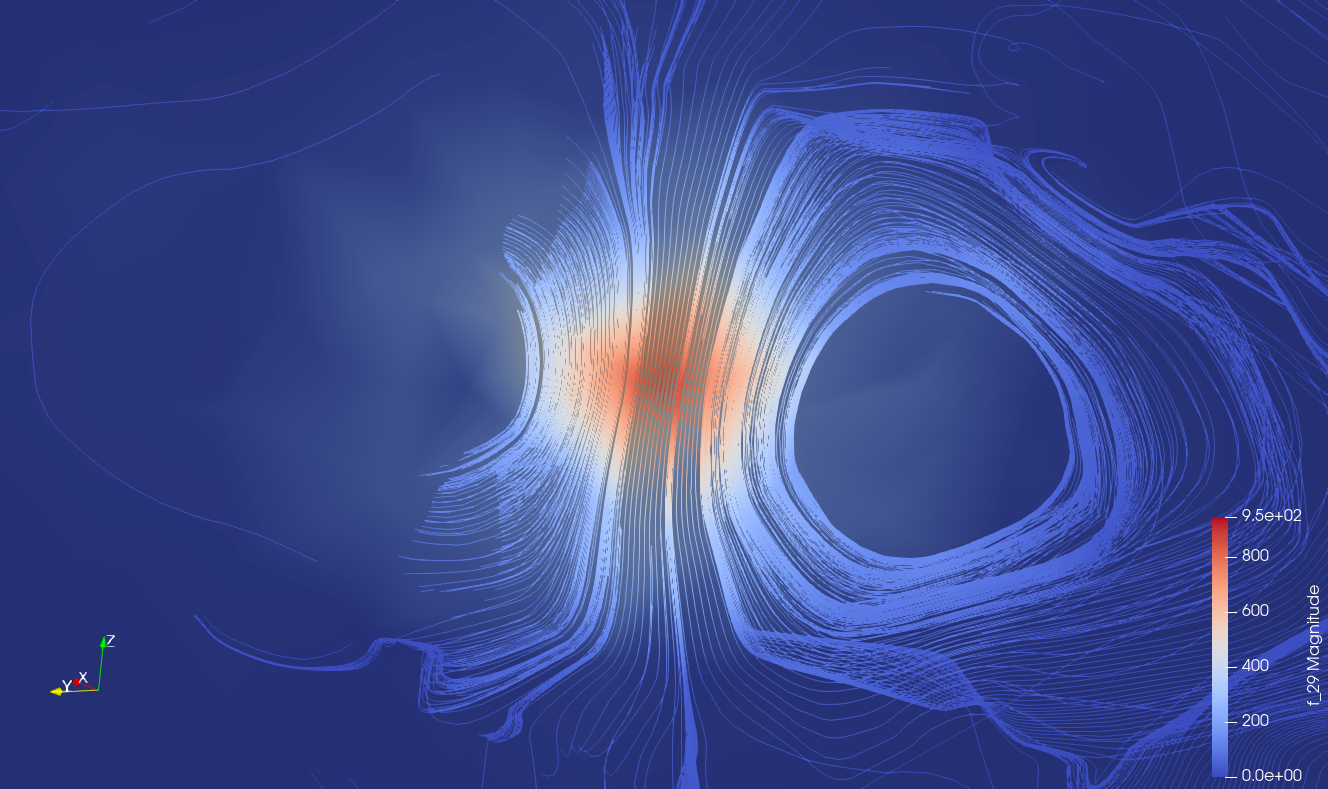
\includegraphics[width=0.45\columnwidth,keepaspectratio]{fenics/test/fenics_coil_B.png}
}%
\label{fig:highm-pos}
\caption{基于 FEniCS 进行的模拟结果}
\end{figure}


% \chapter{Existence and Uniqueness}
\label{cha:exist-unique}

% \chapter{Stability}
\label{cha:stability}
Large amount of attention has been put on the problem of stability of stationary solutions of the Vlasov-Poisson system, both in the stellar dynamics and the plasma physics cases. The energy-Casimir 
method has been used to prove non-linear stability for various conservative systems, and \cite{rein_non-linear_1994} employed the method to prove non-linear stability of the Vlasov-Poisson system in three grometrically different setting. The three settings are the situations where the ion density is replaced by a given fixed ion background, the plasma can be spatially periodic, or can be restricted to a bounded domain. 


With the exception of the first case, stationary solutions exist in these settings and also in the stellar dynamic case. 
In the physics literature there are numerous investigations of the problem of stability of these stationary solutions, both linear and non-linear, and we refer to [1,2]\footnote{Not yet found} and the monographs [4,5]\footnote{Not yet found} for references. In contrast, very little rigorous mathematics exists on this problem. In [2,9]\footnote{Not yet found} non-linear stability of stationary solutions in a spatially periodic, plasma physics setting is established for the Vlasov-Poisson system and the 
relativistic Vlasov-Maxwell system, respectively, see also [lo, 111\footnote{Not yet found}. The problem of linear stability is investigated in [l]\footnote{Not yet found}, both for the plasma physics and the stellar dynamics cases. The phenomenon of Landau damping is established mathematically 
in [ 6 ]\footnote{Not yet found} for the one-dimensional, linearized Vlasov-Poisson system. 
The starting point of the present investigation is a general method to assert 
non-linear stability of stationary solutions for (infinite-dimensional, degenerate) 
Hamiltonian systems, which is presented in [S]\footnote{Not yet found}. We briefly review this method. Let the 
system under consideration be described by the equation of motion 

$$\dot{u} = A(u)$$

on some state space $X , A : D(A) \rightarrow X $ a (non-linear) operator, and let $u_0$ be the 
stationary solution whose stability we want to investigate. The following steps lead to 
a stability result for $u_0$:

\begin{enumerate}
  \item Find the energy (Hamiltonian) $H :X + \bbR$ of the system; $d H ( u ( t ) )/dt = 0$ along 
  solutions. 
  \item Relate $u_0$ to another conserved quantity Casimir functional $C : X + \bbR$ such that $u_0$ is a critical point of $H_C := H + C$, i.e. $DH_C(u_0) = 0$. 
  \item Show that the quadratic part in the expansion of $H_c$ at $u_0$ 
  $$H_C(u) = H_C(u_00) + DH_C(u_0)(u - u_0) + D^2H_C(u_0)(u - u_0, u - u_0) + ... $$
  is positive definite, more precisely, find a norm $|| \cdot ||_a $ on X such that 
  $$H_C(u) - H_C(u_0) - DH_C(u_0)(U - u_0) \geq  C||u-u_0||^2_a \in X,$$ 
  for some $C > 0$. 
  \item Find a norm $||\cdot ||_b$ on $X$ with respect to which $H_c$ is continuous at $u_0$. 
\end{enumerate}


If Steps (1)-(3) can be carried through, then for any solution 

and with Step (4) we conclude that for any $\varepsilon > 0$ there exists $\delta > 0$ such that $||u(0)-u_0||_b < \delta$ implies  $$\left\|u(t)-u_{0}\right\|^{2}_a \leqslant \frac{1}{C}\left|H_{C}(u(0))-H_{C}\left(u_{0}\right)\right| ,$$ \textit{i.e}. $u_0$ is non-linearly stable. 

Though the energy-Casimir method is elegant and appealing, in [S] 
it is pointed out that the appearance of large velocities could cause the method to run into trouble.



%%% 其它部分
\backmatter

%% 本科生要这几个索引,研究生不要。选择性留下。
% 插图索引
\listoffigures
% 表格索引
\listoftables
% 公式索引
\listofequations


%% 参考文献
% 只能选择一种参考文献格式
% \bibliographystyle{thuthesis-numeric}      % 顺序编码制
% \bibliographystyle{thuthesis-author-year}  % 著者-出版年制
\bibliographystyle{thuthesis-bachelor}     % 本科生参考文献的著录格式
\bibliography{ref/refs}


%% 致谢
% 如果使用声明扫描页,将可选参数指定为扫描后的 PDF 文件名,例如:
% \begin{acknowledgement}[scan-statement.pdf]
\begin{acknowledgement}
  衷心感谢导师梁云峰教授给我的毕设选题,它在原理上不是特别困难,是让我熟悉磁拓扑结构很好的练手。其基础的 ERGOS 程序的架构问题确实已经造成了相关研究者很长时间的困扰。从我收到的师兄的反馈而言,重构 ERGOS 的愿望确实较为强烈,于是我的毕设过程中便将其重构了一遍以便于并行化。也许对于单个线圈的分析工作还可以忍受原本的程序架构,但一旦涉及到优化问题中的十余个线圈的协同模拟则会让人感到头疼。梁老师常常抽时间和我一聊就是两三个小时,解答我的疑惑并跟进课题进展。此次所幸题目主要是模拟工作,疫情造成的影响主要在生活琐事上的,与毕设实验的同学相比起来算是幸运了不少。
  
  感谢本科期间高喆教授给我的诸多帮助,不论是本科的学习生活还是研修经历,高喆教授都帮了我许多。我已经占了高老师办公室将近一个年头的工位了,虽然有些不舍得但今年就要搬走了。感谢高喆老师在本科期间对我各种冒失的宽容和支持。谭熠老师在每次组会上也常常和我交流,感谢两位老师在组会上给出的意见。
  
  感谢各位等离子体所认识的师兄师姐,大家在我问问题的时候几乎知无不言,很快就能给我反馈。特别要感谢贾曼妮师姐和张华祥师兄,两位都曾在我的毕设相关方面做过研究,给了我一定程度的帮助。同时还要感谢廖亮师兄和刘少承老师,疫情期间他们常常与我沟通等离子体所的具体情况。

  感谢在全国高性能计算大赛中认识的比赛组织者,中国信通院的郑立同学。文章中的计算任务大部分都是在他提供的服务器上进行运算的,希望我们以后还能长久合作。

  感谢我的家人,如我的二伯母、母亲等亲人,在疫情期间给了我尽可能的支持,起先于湖北家乡过年的日子里确实是非常困难,但所幸终是过去了,那段时间基本都是靠乡里亲人接济着。后来疫情缓解后随父母回到广东,那时国内境况便好了很多。家人的支持使得我能够持之以恒地完成论文,如果没有他们的支持的话这篇论文着实难以为继。


  % 对磁拓扑结构的研究是个可深可浅的课题,这篇文章受限于时间原因主要讨论的是真空场的情况,期待结题后的暑期能够结合磁流体引擎对等离子体反馈做出更进一步的研究。
\end{acknowledgement}


%% 附录
\begin{appendix}
\chapter{外文资料原文}
\label{cha:engorg}

\title{The title of the English paper}

\textbf{Abstract:} As one of the most widely used techniques in operations
research, \emph{ mathematical programming} is defined as a means of maximizing a
quantity known as \emph{bjective function}, subject to a set of constraints
represented by equations and inequalities. Some known subtopics of mathematical
programming are linear programming, nonlinear programming, multiobjective
programming, goal programming, dynamic programming, and multilevel
programming$^{[1]}$.

It is impossible to cover in a single chapter every concept of mathematical
programming. This chapter introduces only the basic concepts and techniques of
mathematical programming such that readers gain an understanding of them
throughout the book$^{[2,3]}$.


\section{Single-Objective Programming}
The general form of single-objective programming (SOP) is written
as follows,
\begin{equation*} % 如果附录中的公式不想让它出现在公式索引中,那就请
                             % 用 equation*
\left\{\begin{array}{l}
\max \,\,f(x)\\[0.1 cm]
\mbox{subject to:} \\ [0.1 cm]
\qquad g_j(x)\le 0,\quad j=1,2,\cdots,p
\end{array}\right.
\end{equation*}
which maximizes a real-valued function $f$ of
$x=(x_1,x_2,\cdots,x_n)$ subject to a set of constraints.

\newcommand\Real{\mathbf{R}}
\newtheorem{mpdef}{Definition}[chapter]
\begin{mpdef}
In SOP, we call $x$ a decision vector, and
$x_1,x_2,\cdots,x_n$ decision variables. The function
$f$ is called the objective function. The set
\begin{equation*}
S=\left\{x\in\Real^n\bigm|g_j(x)\le 0,\,j=1,2,\cdots,p\right\}
\end{equation*}
is called the feasible set. An element $x$ in $S$ is called a
feasible solution.
\end{mpdef}

\newtheorem{mpdefop}[mpdef]{Definition}
\begin{mpdefop}
A feasible solution $x^*$ is called the optimal
solution of SOP if and only if
\begin{equation}
f(x^*)\ge f(x)
\end{equation}
for any feasible solution $x$.
\end{mpdefop}

One of the outstanding contributions to mathematical programming was known as
the Kuhn-Tucker conditions\ref{eq:ktc}. In order to introduce them, let us give
some definitions. An inequality constraint $g_j(x)\le 0$ is said to be active at
a point $x^*$ if $g_j(x^*)=0$. A point $x^*$ satisfying $g_j(x^*)\le 0$ is said
to be regular if the gradient vectors $\nabla g_j(x)$ of all active constraints
are linearly independent.

Let $x^*$ be a regular point of the constraints of SOP and assume that all the
functions $f(x)$ and $g_j(x),j=1,2,\cdots,p$ are differentiable. If $x^*$ is a
local optimal solution, then there exist Lagrange multipliers
$\lambda_j,j=1,2,\cdots,p$ such that the following Kuhn-Tucker conditions hold,
\begin{equation}
\label{eq:ktc}
\left\{\begin{array}{l}
    \nabla f(x^*)-\sum\limits_{j=1}^p\lambda_j\nabla g_j(x^*)=0\\[0.3cm]
    \lambda_jg_j(x^*)=0,\quad j=1,2,\cdots,p\\[0.2cm]
    \lambda_j\ge 0,\quad j=1,2,\cdots,p.
\end{array}\right.
\end{equation}
If all the functions $f(x)$ and $g_j(x),j=1,2,\cdots,p$ are convex and
differentiable, and the point $x^*$ satisfies the Kuhn-Tucker conditions
(\ref{eq:ktc}), then it has been proved that the point $x^*$ is a global optimal
solution of SOP.

\subsection{Linear Programming}
\label{sec:lp}

If the functions $f(x),g_j(x),j=1,2,\cdots,p$ are all linear, then SOP is called
a {\em linear programming}.

The feasible set of linear is always convex. A point $x$ is called an extreme
point of convex set $S$ if $x\in S$ and $x$ cannot be expressed as a convex
combination of two points in $S$. It has been shown that the optimal solution to
linear programming corresponds to an extreme point of its feasible set provided
that the feasible set $S$ is bounded. This fact is the basis of the {\em simplex
  algorithm} which was developed by Dantzig as a very efficient method for
solving linear programming.
\begin{table}[ht]
\centering
  \centering
  \caption*{Table~1\hskip1em This is an example for manually numbered table, which
    would not appear in the list of tables}
  \label{tab:badtabular2}
  \begin{tabular}[c]{|m{1.5cm}|c|c|c|c|c|c|}\hline
    \multicolumn{2}{|c|}{Network Topology} & \# of nodes &
    \multicolumn{3}{c|}{\# of clients} & Server \\\hline
    GT-ITM & Waxman Transit-Stub & 600 &
    \multirow{2}{2em}{2\%}&
    \multirow{2}{2em}{10\%}&
    \multirow{2}{2em}{50\%}&
    \multirow{2}{1.2in}{Max. Connectivity}\\\cline{1-3}
    \multicolumn{2}{|c|}{Inet-2.1} & 6000 & & & &\\\hline
    \multirow{2}{1.5cm}{Xue} & Rui  & Ni &\multicolumn{4}{c|}{\multirow{2}*{\thuthesis}}\\\cline{2-3}
    & \multicolumn{2}{c|}{ABCDEF} &\multicolumn{4}{c|}{} \\\hline
\end{tabular}
\end{table}

\subsection{Nonlinear Programming}

If at l EAST  one of the functions $f(x),g_j(x),j=1,2,\cdots,p$ is nonlinear, then
SOP is called a {\em nonlinear programming}.

A large number of classical optimization methods have been developed to treat
special-structural nonlinear programming based on the mathematical theory
concerned with analyzing the structure of problems.
\begin{figure}[h]
  \centering
  \includegraphics{thu-lib-logo.pdf}
  \caption*{Figure~1\quad This is an example for manually numbered figure,
    which would not appear in the list of figures}
  \label{tab:badfigure2}
\end{figure}

Now we consider a nonlinear programming which is confronted solely with
maximizing a real-valued function with domain $\Real^n$.  Whether derivatives are
available or not, the usual strategy is first to select a point in $\Real^n$ which
is thought to be the most likely place where the maximum exists. If there is no
information available on which to base such a selection, a point is chosen at
random. From this first point an attempt is made to construct a sequence of
points, each of which yields an improved objective function value over its
predecessor. The next point to be added to the sequence is chosen by analyzing
the behavior of the function at the previous points. This construction continues
until some termination criterion is met. Methods based upon this strategy are
called {\em ascent methods}, which can be classified as {\em direct methods},
{\em gradient methods}, and {\em Hessian methods} according to the information
about the behavior of objective function $f$. Direct methods require only that
the function can be evaluated at each point. Gradient methods require the
evaluation of first derivatives of $f$. Hessian methods require the evaluation
of second derivatives. In fact, there is no superior method for all
problems. The efficiency of a method is very much dependent upon the objective
function.

\subsection{Integer Programming}

{\em Integer programming} is a special mathematical programming in which all of
the variables are assumed to be only integer values. When there are not only
integer variables but also conventional continuous variables, we call it {\em
  mixed integer programming}. If all the variables are assumed either 0 or 1,
then the problem is termed a {\em zero-one programming}. Although integer
programming can be solved by an {\em exhaustive enumeration} theoretically, it
is impractical to solve realistically sized integer programming problems. The
most successful algorithm so far found to solve integer programming is called
the {\em branch-and-bound enumeration} developed by Balas (1965) and Dakin
(1965). The other technique to integer programming is the {\em cutting plane
  method} developed by Gomory (1959).

\hfill\textit{Uncertain Programming\/}\quad(\textsl{BaoDing Liu, 2006.2})

\section*{References}
\noindent{\itshape NOTE: These references are only for demonstration. They are
  not real citations in the original text.}

\begin{translationbib}
\item Donald E. Knuth. The \TeX book. Addison-Wesley, 1984. ISBN: 0-201-13448-9
\item Paul W. Abrahams, Karl Berry and Kathryn A. Hargreaves. \TeX\ for the
  Impatient. Addison-Wesley, 1990. ISBN: 0-201-51375-7
\item David Salomon. The advanced \TeX book.  New York : Springer, 1995. ISBN:0-387-94556-3
\end{translationbib}

\chapter{外文资料的调研阅读报告或书面翻译}

\title{英文资料的中文标题}

{\heiti 摘要:} 本章为外文资料翻译内容。如果有摘要可以直接写上来,这部分好像没有
明确的规定。

\section{单目标规划}
北冥有鱼,其名为鲲。鲲之大,不知其几千里也。化而为鸟,其名为鹏。鹏之背,不知其几
千里也。怒而飞,其翼若垂天之云。是鸟也,海运则将徙于南冥。南冥者,天池也。
\begin{equation}\tag*{(123)}
 p(y|\mathbf{x}) = \frac{p(\mathbf{x},y)}{p(\mathbf{x})}=
\frac{p(\mathbf{x}|y)p(y)}{p(\mathbf{x})}
\end{equation}

吾生也有涯,而知也无涯。以有涯随无涯,殆已!已而为知者,殆而已矣!为善无近名,为
恶无近刑,缘督以为经,可以保身,可以全生,可以养亲,可以尽年。

\subsection{线性规划}
庖丁为文惠君解牛,手之所触,肩之所倚,足之所履,膝之所倚,砉然响然,奏刀騞然,莫
不中音,合于桑林之舞,乃中经首之会。
\begin{table}[ht]
\centering
  \centering
  \caption*{表~1\hskip1em 这是手动编号但不出现在索引中的一个表格例子}
  \label{tab:badtabular3}
  \begin{tabular}[c]{|m{1.5cm}|c|c|c|c|c|c|}\hline
    \multicolumn{2}{|c|}{Network Topology} & \# of nodes &
    \multicolumn{3}{c|}{\# of clients} & Server \\\hline
    GT-ITM & Waxman Transit-Stub & 600 &
    \multirow{2}{2em}{2\%}&
    \multirow{2}{2em}{10\%}&
    \multirow{2}{2em}{50\%}&
    \multirow{2}{1.2in}{Max. Connectivity}\\\cline{1-3}
    \multicolumn{2}{|c|}{Inet-2.1} & 6000 & & & &\\\hline
    \multirow{2}{1.5cm}{Xue} & Rui  & Ni &\multicolumn{4}{c|}{\multirow{2}*{\thuthesis}}\\\cline{2-3}
    & \multicolumn{2}{c|}{ABCDEF} &\multicolumn{4}{c|}{} \\\hline
\end{tabular}
\end{table}

文惠君曰:“嘻,善哉!技盖至此乎?”庖丁释刀对曰:“臣之所好者道也,进乎技矣。始臣之
解牛之时,所见无非全牛者;三年之后,未尝见全牛也;方今之时,臣以神遇而不以目视,
官知止而神欲行。依乎天理,批大郤,导大窾,因其固然。技经肯綮之未尝,而况大坬乎!
良庖岁更刀,割也;族庖月更刀,折也;今臣之刀十九年矣,所解数千牛矣,而刀刃若新发
于硎。彼节者有间而刀刃者无厚,以无厚入有间,恢恢乎其于游刃必有余地矣。是以十九年
而刀刃若新发于硎。虽然,每至于族,吾见其难为,怵然为戒,视为止,行为迟,动刀甚微,
謋然已解,如土委地。提刀而立,为之而四顾,为之踌躇满志,善刀而藏之。”

文惠君曰:“善哉!吾闻庖丁之言,得养生焉。”


\subsection{非线性规划}
孔子与柳下季为友,柳下季之弟名曰盗跖。盗跖从卒九千人,横行天下,侵暴诸侯。穴室枢
户,驱人牛马,取人妇女。贪得忘亲,不顾父母兄弟,不祭先祖。所过之邑,大国守城,小
国入保,万民苦之。孔子谓柳下季曰:“夫为人父者,必能诏其子;为人兄者,必能教其弟。
若父不能诏其子,兄不能教其弟,则无贵父子兄弟之亲矣。今先生,世之才士也,弟为盗
跖,为天下害,而弗能教也,丘窃为先生羞之。丘请为先生往说之。”
\begin{figure}[h]
  \centering
  \includegraphics{thu-whole-logo.pdf}
  \caption*{图~1\hskip1em 这是手动编号但不出现索引中的图片的例子}
  \label{tab:badfigure3}
\end{figure}

柳下季曰:“先生言为人父者必能诏其子,为人兄者必能教其弟,若子不听父之诏,弟不受
兄之教,虽今先生之辩,将奈之何哉?且跖之为人也,心如涌泉,意如飘风,强足以距敌,
辩足以饰非。顺其心则喜,逆其心则怒,易辱人以言。先生必无往。”

孔子不听,颜回为驭,子贡为右,往见盗跖。


\title{ EAST  托卡马克上低杂波引起的磁拓扑变化,及其对边界局域模的显著影响}

{\heiti 摘要:} 当低杂波和离子回旋共振加热作用在 H-mode 的等离子体,在  EAST  上观测到了强烈的减弱边界局域模的作用。这种效果是由于低杂波引起的螺旋电流丝沿着磁力线在刮削层中不断流动的效果。和共轭磁扰动的效果类似,在低杂波运作期间也出现了束流在偏滤器上落点分裂的现象。通过在磁力线追踪程序中加入螺旋电流丝,本文也定性地模拟了其对磁拓扑结构的改变的作用。

% TODO Add figure & citation


对聚变能源研究及相关技术的巨大挑战来自于如何将炽热的等离子体约束住,使得接触等离子体的材料在运行期间维持一个可以接受(稳态和瞬态)的热负荷及粒子束流强度。
当托卡马克中的等离子体工作在高约束(\Hmode)状态的时候,等离子体能量约束时间显著增长。然而其后果则是等离子体边界上压强有着更大的梯度,连带着还有边界上增强了的电流密度,它可以超过阈值以驱动磁流体不稳定性,这被称为边界局域模。边界局域模会导致近似周期性的大量能量和粒子从本应受约束的区域损失,同时又会导致对接触的等离子体材料的严重损害,下一代的聚变设备,如 ITER 和 DEMO 装置,需要一种可靠的手段来控制或者抑制剧烈的边界区域模。

共轭磁扰动(RMP)改变了等离子体的磁拓扑结构,已经被用在 DIII-D 装置内完全抑制边界局域模,或者在实验中,抑制边界区域,这个的意思是增加边界局域模的频率,而减低每一次边界局域模发生的幅度,must和ORG装置上面得到实验。尽管这个物理机制还不是很清楚,。不同装置上得到的实验结果都表明是拓扑,有着一个很关键的作用,在整体约束中,以及边界磁流体稳定性,何等的相互作用,特别是对于,偏滤器


目前来说,在所有现存的以共轭磁扰动减弱或抑制边界局域模的实验中,磁扰动均由腔内或者腔外的线圈系统所激发。腔内的磁扰动线圈已在 ITER 设计上被考虑并做出了设计,用于抑制边界局域模的发生。但在未来的聚变反应堆中,(DEMO)腔内的磁扰动线圈可能不现实。于是通过其他机制改变磁拓扑来控制边界局域模,对于下一代的托克马克提供了一个有吸引力的解决方案。

最近 EAST 上面的研究结果表明,低杂波和共轭磁扰动的效果类似,通过改变磁拓扑,可以作为一种有效的减弱或者抑制边界局域模的手段。这篇快报阐述了低杂波对边界局域模表现的影响及偏滤器平板上的热负荷分布;同时记录了低杂波驱动下产生的,在刮削层中沿着磁力线流动的螺旋电流丝的实验结果(该螺旋电流丝并不随时间旋转)。观测到的由螺旋电流丝引起的三维边界磁拓扑改变和磁力线迹线程序所做的估计之间进行了对比。

EAST (大半径和小半径分别是 \SI{1.85}{\metre} 和 \SI{0.45}{\metre}) 是为了实验稳定的长脉冲、高参数的 H-mode 等离子体而建造的装置,它的位型与加热设备 ITER 类似,即有着灵活可调的 double null, lower single null (SN) 或 upper (SN) 极向偏滤器位型并主要是射频加热。EAST 中的低杂波系统工作在 \SI{2.45}{\giga\hertz},一个阵列由 20 个波导天线组成,四列五行,安装在低场侧中间,最大输出功率是 \SI{2}{\mega\watt}。其最初被设计用于芯部等离子体电流驱动,通过将电子朗道阻尼将动量转移给等离子体。峰值平行方向波折射率约 2.1。并且这套低杂波系统可以在没有离子回旋共振加热(ion cyclotron resonance heating, ICRH)的条件下仍实现长脉冲下的\Hmode 。然而和其他设备上的实验类似,显著的低杂波功率会损失在等离子体边界上面,特别是当等离子体密度较高时,这是由快波和粒子之间复杂的耦合问题所导致的。

低杂波对于边界局域模的特性影响,通过在离子回旋共振加热占主导的\Hmode 等离子体中调制低杂波功率中进行了研究。在这项实验中,目标 \Hmode 等于几?有一个,下SM配置这个高\Hmode 等议题主要是由你只会控制驱动的,他的输入功率是 \SI{1}{\mega\watt},在一个相对高密度的区域啊,在礼毕包成之后,problem。在边界上的安全系数是3.8。同时还有一个还相等于是电流在500千左右,以及还现场,1.8特斯拉,底部的三角系数是0.45。在等式中中心线密度的平均密度10是4.7×10的19次幂\SI{4.7}{},每立方米,以及,Greenwald 系数约 0.9,H 系数(H98y)在 \Hmode 阶段约 0.8。

这套低杂波系统功率设置在 \SI{1.3}{\mega\watt}。调制频率为 \SI{10}{\hertz}。运转时长占周期比例 50\%,于是,低杂波关闭的一个项相位时间是\SI{50}{\milli\second},这个时间大概是能量约束时间的一半,如果没有低杂波系统的话,边界局域模的频率是非常规律的,大概在 \SI{150}{\hertz}左右,当低杂波系统打开之后,人家就用膜消失了,或者problem,很奇怪的,出现在一个非常高的频率,大概在600号之后只左右,如图一所见。边界局域模,风之利刃,刘强出现了显著的下降。大概有一个因子,2,并且有一个显著的增强在边界局域模之间的粒子数强,也是系数大约是。但仍然低于在l模工作室。这一现象在p7平板上面观测到了,在使用低杂波的时候,。等于其所具有的能量,大概有一个,因此为2的涨幅,从五十千焦到一百千焦,一旦\Hmode 。一旦\Hmode 成功啊。并且在低杂波功率调制期间,它的变化幅度比较微弱,大概在$\pm 5\%$区间之内。只有两个天然气平板所接收到的女子刘蔷,一旦关闭了低杂波系统,就会有一个迅速的衰弱,这可能揭示着低杂波功率,不仅仅是在本心不被吸收,同时他也,沉积在了刮削层中。

EAST 实验中,不管是\Lmode 还是\Hmode ,低杂波运行期间刮削层中都观测到了 5 条螺旋辐射带(Helical radiation belt, HRB)。螺旋辐射带的数量和低杂波天线阵列的行数是一样的。EAST 使用氦气放电使其结构更清楚而不改变其总的特性。作为一个典型例子,图 2 表示了两个切向方向上可见光波段的照片,这是氦气等离子体放电过程中,从 EAST 环形腔两侧 低杂波应用过程中所出现的图片。



这艺术目标等于几,300千安,磁感应强度两个特斯拉,$B=\SI{2}{\tesla}$, $q=0$安全系数为8左右,试油等,是由低杂波加热,大概功率有 \SI{0.7}{\mega\watt},他的拓普卫星是一个 double null 的配置。再等一日起,分割面以及,外层中央平面显示器之间的间隔大概在 \SI{8}{\centi\metre}。螺旋辐射带,沿着刮削层流动,在低场次,他同时向上面和下面的偏滤器,沿着磁场线同时流动,在天线前面。p刮削层中的磁力线,大概在等于己边界一厘米之外,就在低杂波天线前面。实验和模拟计算结果在位置和 pitch 角度上面都有很好的吻合。

% FIXME pitch angle

在等离子体边界螺旋丝状结构中流动的电流所激发出来的磁扰动,已经通过 Mirnov 线圈观测到了,发生在低杂波系统调试过程中。在这项实验中低杂波功率,用方波对它进行调整,功率周期性在\SIrange{0}{1.2}{\mega\watt}之间转换,它的重复频率是\SI{100}{\hertz},运转时长占周期 50\%。螺旋电流丝的产生是相当快速的,约\SI{2}{\milli\second}之内,这么短的时间对应着低杂波系统的启动时间。这就是系统开始的时候,螺旋电流丝,电流好散,在几个毫秒之内,电流丝所启动的拓朴结构改变,是在极向和环向上都是对称的,它表明了。等离子体结构的三维扭曲,。总的螺旋电流丝,电流强度。可以通过乔昌江模拟中,计算的扰动场强度与实验中的进行配合,被发现它的强度在。左右,在这项实验中。

在偏滤器上落点(Strike points, SP)的分裂,在低杂波加热系统运转的时候被观测到了。其分裂落点的效果和共轭磁扰动相似,可以在偏滤器平板上的热负荷分布上所观察到。图 4 显示了通过一个红外摄像头测量的外侧下部偏滤器平板的表面温度。平板上面,热负荷。。参照图片是。在低杂波使用过程中,外侧低处的天然气平板上面,表面温度,他表现出一个和原有的打击点,所截然不同的多分裂模式。间的距离,取决于环向角,这表明低杂波造成的磁拓扑是三维结构。另外落点分裂还取决于边界的安全系数,这一点,欧姆加热主导的和离子回旋加热主导的等离子体中都没有发现。
% FIXME Connection Length
% FIXME equilibrium 
% FIXME lobe
通过在磁力场线追踪的程序中考虑螺旋电流丝,如图 5 ,本文定性地模拟了磁拓扑结构的改变。在实验平衡态磁场基础上,加上从螺旋电流丝来的磁扰动场,电流丝测量到的电流强度为 \SI{1.3}{\kilo\ampere},以此来计算磁力线的重联长度。螺旋电流丝产生的磁场,在 X 点附近形成了数瓣有着较长重联长度的磁力线,直达外侧偏滤器平板造成打击点的分裂,使得落点发生了分裂,这一过程被红外摄像头所识别。计算结果表明,等离子体边界的剧烈变化,取决于边界的安全系数,和流经电流丝的电流强度。还要注意该螺旋电流丝模型没有考虑进去等离子体反馈,并且模拟的结果,只能定性地解释,螺旋电流丝激引起的落点分裂。
% FIXME small ELM
过去的的实验结果已经表明低杂波可以引起震荡型的边界局域模\Hmode 在 SN 偏滤器位型上(JET),也可以在限制器位型下产生没有边界局域模的\Hmode 等离子体(JT60),然而,它具体的物理机制还没有被充分研究。在 EAST 上,对离子回旋共振加热占主导的较低密度等离子体($n_e/n^{GW}<0.5$,这里 $n^{GW}$ 为 Greenwald 密度极限),用恒定的低杂波功率可以得到一个边界局域模较平稳的\Hmode 等离子体,其边界局域模有着混合的 type-I 和小类型的。通过降低离子回旋共振加热对低杂波加热的比例,再提高等离子体密度,达到了一个持续发生小类型边界局域模的\Hmode 等离子体,并且保持了32秒。低杂波激发的螺旋电流丝及其造成的磁拓扑改变迹象合理地解释了为什么低杂波可以减弱或者抑制边界局域模,并且显著地改变对偏滤器平板上的热负荷分布。对于这种现象背后物理机制的理解,需要考虑这种抑制效果关于以下几个因素的依赖关系,(i) 锂壁涂层,(ii) 等离子体碰撞,(iii) 安全系数,它们将会在未来 EAST 上的实验进行进一步的研究。

由于低杂波天线几何因素的影响,由螺旋电流丝所驱动的共轭磁扰动场主要是 n=1 的分量,在这里 n 指环向模数。基于实验参数计算出来的磁扰动场的谱表明螺旋电流丝的次扰动场共轭能力较好,从图 6 中可以看到,等离子体边界共振面和共轭磁扰动途中的脊线相贴合的。另外,由螺旋电流丝所引起的磁扰动,更多地位于等离子体边界,没有对核心部分显著的影响,这主要是由于螺旋电流丝在等离子体边界的刮削层中沿着磁力线进行流动。因此,螺旋电流丝的迹线总是紧密地贴合着边界磁力线的 pitch,而与边界安全系数无关。

还需要提到,尽管低杂波在刮削层中引起电流的现象已经被许多设备上观察到了,然而它的物理机制依然不清楚,在 Alcator C-Mod 的实验装置上面,当我们将低杂波注入方向改变的时候,刮削层中的电流方向并不会发生改变。Alcator C-Mod 上,在低杂波功率约 \SI{850}{\kilo\watt} 时,若等离子体运转在高密度状态,在刮削层中估计电流强度可以高达约 \SI{20}{\kilo\ampere},而 EAST 上低杂波功率为 \SI{1.3}{\mega\watt} 时,极向上积分得到的螺旋电流丝则约\SI{7}{\kilo\ampere}。
用 GENRAY-CQL3D 程序对考虑碰撞阻尼的二维刮削层模型模拟表明,EAST 上运行的高密度等离子体, 大概 10\% 的低杂波功率沉积在了刮削层中。实验观测到的结果,表明刮削层中的电流过大以至于不能通过直接的电流驱动,,引起对低杂波的碰撞吸收,来解释,不过要注意,刮削层中的低杂波功率吸收会对偏滤器区域中性粒子的电离有所贡献,从而增强了,沿着刮削层中的磁力线从较热较稀疏的偏滤器平板到较冷较稠密的偏滤器平板的热电电流,。
% thermoelectric current
EAST 过去的研究表明,随着低杂波功率或者等离子体密度的增长,螺旋电流丝电流强度均会增长。然而,螺旋电流丝所处的径向位置在刮削层中的分割面附近,而此处重联的磁场线长度远远大于电子的平均自由程。为了用低杂波实现对边界局域模和偏滤器平板上热负荷主动的控制,螺旋丝中电流强度对实验参数的依赖关系将会在 EAST 上面更进一步地被研究。

总的来说,低杂波对于边界局域模强烈的影响已经在 EAST 上面得到了呈现,它表明边界局域模在其作用下会消失,或者偶尔出现,它的频率会从 ~150 增加到 ~\SI{600}{\hertz},当低杂波进行驱动的时候,低杂波似乎通过驱动沿着刮削层磁力线且不随时间环向旋转的螺旋电流丝,来引起磁拓扑上显著的改变。这导致了在偏滤器上的落点分裂,与共轭磁扰动引起的效果相仿。在磁力线追踪程序中引入螺旋电流丝能较好地复现出来磁拓扑所观测到的改变。这为下一代的聚变反应堆(ITER 或 DEMO)提供了一种很有吸引力的手段来优化热负荷分布,并且同时抑制或者削弱边界局域模导致的极大的瞬态热负荷和粒子流强。

这项研究由中国国家磁约束聚变科学项目支持,项目序号为 No. 2013GB106003 和 No. 2011GB107001。在这里还要致谢德国亥姆霍兹协会的亥姆霍兹大学青年研究者团体  VH-NG-410。



\title{EAST 托卡马克上共振磁扰动驱动的从削弱边界局域模到完全抑制的非线性转换}

{\heiti 摘要:} 本文呈现了 EAST 托卡马克上如何用共轭磁扰动使得边界局域模从被减弱到被抑制住的非线性转换。这是第一次对射频加热占主导且缓慢旋转的等离子体的边界局域模用共轭磁扰动的方法进行抑制。在转化发生之后,边界磁拓扑的改变有两个迹象,线性磁流体动力学和真空的模拟结果等离子体反馈场渐变的相移和骤然的射向偏滤器的三维粒子束流。转换的阈值依赖于共轭磁扰动场的磁谱、等离子体自身的旋转及扰动场的幅度。这表明非线性等离子体反馈引起的边界磁拓扑结构改变在用共轭磁扰动的手段抑制边界局域模时很重要。


无论是在实验室等离子体物理研究中还是在空间等离子体物理研究中,磁场重联及其导致的拓扑变化在等离子体动力学中扮演了一个重要角色。通过共振磁扰动所引起的边界随机场,被认为是抑制等离子体边界周期性 crash 发生的合理理由,其也被称为边界局域模,在 DIII-D 托卡马克中,边界局域模会导致瞬态的热负荷,到等离子体,到直接面对等你写的材料中,并且可能使得它们性能下降,并且可能导致他们无法完成,工作在下一代的,即便设备中。在边界压力梯度和电流中储存的自由能,他们可能会由于产的随机性而减小的随机性加等于几?引入一个更稳定的区间,来对抗边界局域模,这样成功的实验,促进了边界局域模控制的技术发展,通过。共轭。共轭磁扰动。然而等离子体的响应效应,通常会屏蔽,外界施加的共轭磁扰动,并且写可能显著的,减低磁场的随机性,这使得这一机制能否应用德打上了一个问号。我洗碗了。与拓朴结构的改变不同,线性的feeling like10磁流体动力学响应,已经被发现扮演了一个重要的角色在边界局域模控制中,非线性的等离子体响应,已经在jet托卡马克中被观测到了。然而,在边界局域模被完全抑制和削弱之间的关键性区别仍不清楚,以及线性和非线性的等离子体反馈在边界局域模抑制上的作用仍有待研究。

,在这篇快报中,我们报告了。列举一模完全的意志,通过外置的低的,放置于底部的,嗯,环向傅立叶魔术n等于n的共轭磁扰动,在缓慢的旋转的本体中,他有着射频波加热主导的加热机制,这可能对于这项技术在未来聚变设备上的应用,有着较为重要,有着潜在的重要价值,这是第1次观测到,完全的边界局域模一致,通过共轭磁扰动,在介质等离子体碰撞区在等车中,并且它拓展了之前,边界局域模一致的观测结果,在DC和Kstar上面。?我发现。不仅是在边界附近的磁场还有超过一支水平的词,托福改变,包括等离子体响应都在最终的边界局域模一事中起着重要作用,这一发现也揭示了,在线性和非线性响应效应中,非线性和非线性响应,在边界局域模意志中的不同角色。一套灵活的腔内,工作场线圈系统,包括两个阵列,2×8=16,安装在低场侧,在超导托卡马克 EAST 中,于2014年,我们已经成功的实现了,包括意志和完全的消除,一类型的边界局域模,通过环向傅立叶,4=1的和2的共轭线圈在缓慢的旋转的等离子体,这个等离子体的加热是由射频波主导的,在 EAST 托卡马克中。完全的边界局域模一致通过环向傅立叶魔术,n等于1的共轭产线圈。被观测到在完全的视频锅加热,等于是体重在一食堂里面,当扰动场强度超过了一个阈值的时候,图1显示,边界局域模的表现在缓慢的启动过程中n等于1的,共轭线圈,宫娥共轭磁扰动产线圈,共轭老动线圈电流中,在 EAST 内,序号为55274,额外的加热功率来自于低杂波电流驱动的,其功率为三个兆瓦,以及离子回旋共振加热。粒子回旋共振,加热功率为1.4个照啊,保持着常速。方向上的旋转在等离子体中心,非常接近于0,小于4,k微点,通过x射线晶体成像技术,环向强度为2.25个特斯拉,在表面上的安全因子。其95\%的正规划极向场,刘强,q95约等于5.7,等离子体电流等于0.45个照安培,规划的贝塔为0.8,以及规划的碰撞率在平台顶部是差不多,约等于1,就如图一所示。像一个阶梯一样的,电子密度减弱,以及边界局域模频率的增强,都在共轭线圈应用的时候被观测到了,在他升到8000陪之前,而在边界局域模完全被抑制之,在此之后边界局域模被完全的抑制住了。

真空模拟的磁场强度,占据的面积,已经在图一中得到呈现,在这里试试参数表示指导纯洁的条件和市政规划的,规划过了的,极向直通。等离子体响应,在边界局域模的削弱和抑制阶段是完完全全是非常显著的不同。n=1共轭磁扰动场的幅度,由于试题响应所造成的,在实验中观测到的结果,但通过词。测量在图一中得到的结果如图所示,像台阶一样的,电子密度下降趋势以及边界局域模频率的增长,在完全的抑制之前,可能是由于不同谐波频率的穿透,他们有着不同的穿透日子,这表明,磁拓扑结构改变的程度,也考虑,如果把,也将等于直接响应考虑进来,在最终的边界局域模日记中扮演了一个重要的角色,这。激励我们进一步的研究,细致的等级响应,演化过程在边界局域模的削弱和意志之间转化。边界局域模的削弱和解粒子转化过程中,被单线圈和下线圈的相位差扫描所检测到,你们。明天就走了,或者等价的。通过共振分量的强度来观测,徒儿展示了边界局域模控制机制,我们有一个连续性的扫描,相差。通过旋转下面的线圈电流,再一个,\SI{0.5}{\hertz}的频率,并且保持上面的线圈电流禁止,有一个常数的幅度,嗯,一个千安培。该目标等离子体,有着边界局域模的频率大概在100赫兹左右。和另一个括号中的情况是类似的,除了有一点点在加热机制上的不一样,及。他有着 \SI{0.7}{\mega\ampere} 的反向电流,中性束注入,而不是电子回旋共振加热,它仍然是射频主导的加热等离子体,电子密度的改变。和边界局域模频率,可重复性比较好,在两个阶段。它有着明显的33各项阶段,在第1个阶段。强烈的密度和边界局域模削弱,但是边界局域模的频率增强了,因此大概在5~10左右膜再向阶段二中完全的抑制住了,在一个突然的电子密度下落之后,在第三阶段,相位差的其余部分。相当相当弱,并且总是保持着一个阐述在一个突然的转换中,边界局域模意志中,拖出来,电子密度和温度。形貌的变化,在图中有所展示。从中我们可以看到电子密度下降了,但温度上升了,在工厂缠绕中的应用阶段,等离子体能量约束,在边界局域模的意义削弱中,是似乎有一些轻微的便好,更多的储存能量,当然更低的密度。比赛共轭磁扰动,应用之前要好,和边界局域模的意志相削弱相比,完全的抑制,有一个更强,强得多的密度潘博奥效应,和一个轻微的。边界平台温度下降,能量约束,下降了大约10\%,从边界局域模的削弱到完全抑制阶段。边界局域模控制效果的普依赖性表明的,嗯,中达到了一个玉字,是一个必要条件对于共轭磁扰动的抑制效果,而在另一个实验装置中观测到的类似最好的相位差,对于边界局域模意志来说,和共振分子接近,通过这次通过,谢谢磁流体扰动磁流体动力学模拟程序,模拟得到的结果类似,而这个适合真空中共振分子计算出来的,结果是不一样的,然而,。等离子体密度的时间演化,是一个完全不同的。何在,低CD上观测到的结果完全不同,实验中观测到的等于是体密度,潘博奥和词,磁场规定,总是改变,像一个波函数,在相位差扫描过程中,这表明线性的等一级响应,在动力学中的变化。

实验测量结果表明,我们有直接的证据说明,非线性的等级响应和非线性的转化或者分叉,在边界局域模削弱和抑制之间。观测到的等离子体反馈场演化是通过全套的环向阵列极向磁场感应传感器在低场次,图如图三所示,主要的分量是傅立叶魔术,环向魔术等于1的谐谐波量,通过傅立叶分解,这个,嗯,反馈厂。共轭磁扰动产出等离子体响应,通过 MASS-F code模拟出来的结果,在图三中,较好的重现了总体的趋势,观测到的总体趋势,有一点小小的不一样。在时间等于3.9秒,套数为55272的平衡态中,这被用来做。下面的模拟,由于没有显著的变化,在等离子体响应预测上,在等你一起享用上,预测试通过,用一种不同的平衡态,有或者没有,磁扰动的边界局域模抑制效应,在饭店中发现,然而。这表明共振磁扰动被屏蔽掉了,在边界局域模的削弱过程中,和。啊,跟着局玉磨完全抑制阶段,这个穿透却可以发生,这是因为穿透的共振,分量有相同的相位。和真空中的一样,儿臣地产有一个相位偏上位,偏宜相对于真空的那一个,在前面的非线性模拟中预测的,这意味着,最终的黑边界局域模意志,需要铲穿透,我这不能通过线性模拟来揭示,这也能够解释,这可能也能解释一个类似的差别在我在d市第一中,1~11月中所观测到的,穿透效应不一样,在这里穿透的分量职场环向模式数目,适合贝斯佳的一样。



反馈场的相位逐渐的和真空箱真空厂商为不断逼近,而这工厂是从边界局域模削弱到完全一致,过程中,就如图 4 所示。

这表明不同的谐频分量穿透轮回穿透。并且。边界拓扑变化增强了,在这一阶段逐渐增强,穿透了阈值,对于不同的截屏分量来说可能是不一样的,因此,一个可能的解释是,这里有。对于不同的谐频分量来说,穿透阈值可能是不一样的。于是一种可能的,因此一种可能的理由是,有多种截屏分量,一次穿透,在这个转化过程中再解释了,这也解释了,像阶梯一样的电子密度转化。和边界局域模频率变化,在共轭产,共磁扰动电流,上山之前,在最终的边界局域模完全抑制之前,就如图一所示。因此边界,拓扑结构的改变程度,逐渐增强,随着总的共轭死共轭磁扰动,幅度增强,这包括了等离子体反馈,和,并且它导致了最终的边界局域模意志。突然的反向转化从跟着局玉磨抑制,二阶段到比较弱的边界局域模削弱阶段表明这些共振分量,中证,谐频分量,又再一次被屏蔽掉了,几乎同时,并且三维的资产结构消失了,单总的共轭持,共轭磁扰动强度变的,低于一个月之后。。在边界局域模抑制阶段,由共轭磁扰动引起的粒子流强打击在偏滤器上的落点的分裂,和边界拓扑结构改变的变化是一致的,三维的打击点,旨在本人实体屏蔽效应削弱的时候,被观测到在l模等离子体滴滴设置中,共轭磁扰动产,超过一个月之后,一个三维的打击点,不管是粒子刘强还是热敷后的刘强,热负荷,在偏滤器上,都伴随着一个突然的热负荷增强和等离子体密度的减弱,这表明边界随机性的形成,这已经在l模等离子体中被观测到了在max上面。这种分裂模式再强的边界局域模削弱阶段和抑制阶段,被观测到时用一个极向阵列的兰缪探针,在上偏滤器,在phi角等于327度的时候,观测到图3,这和真空的三维模拟,打几点去的?结果是相吻合的,显著的粒子流强增加,也表明了俺的穿透和磁拓扑结构改变,在这些阶段,因为这是一个机的sn味型,其中的两个分割面之间的距离大概在一厘米,再一次说明了,边界拓谱的改变,在边界局域模,抑制发生的时候。

。边界垂直转动,有一个额外的增加都在从边界局域模削弱到完全抑制过程中,被观测到了,这再一次说明,边界痛苦的拓扑结构改变的重要性,完全的抑制的时候。边界转动的加速。是边界随机性形成的一个证据图5显示了一个对比,边界局域模控制效果在两个数之间,他们有着相同的,共轭磁扰动为行,和目标等于日期,磁场强度为1.7特斯拉,电流0.45兆安培贝塔n约等于1.5和q95,约等于4.5,除了。那也行,顺电流方向的。中性束,功率为。从两个兆瓦到1.2的照啊,就如图5所示,一个阶梯,旋转共轭此共轭磁扰动,有着这样子的类型,相位保持着常速的电流7度。在这两个号上面都有所应用,强烈的边界局域模削弱,大概是有一个因子5\%。嗯。嗯,以及一个。以及边界局域模频率的增长,被观测到了,在共轭磁扰动的应用之后,完全的词跟我完全的,嗯,边界局域模抑制,只有在一个额外的瞬间增长,什么增长呢?边界垂直旋转增长之后才会实现在一个缓慢的衰弱,等一起旋转衰弱之后,由于这个中性束功率的衰减,然后米尔诺夫信号,被用来作为一种测量手段。表明边界局域模的破裂,因为它是更加对小的边界局域模破裂敏感,在强削弱的时候,如图五所示。边界垂直旋转的突然增加,用多普勒反射系统观测到了,立刻在共轭磁扰动应用之后,这表明,边界拓扑结构的改变,就如图5所示,受评估的电子流起,垂直旋转,何时电场搭乘磁场?在平台顶部变得非常接近于0,在应用了共轭辞共轭磁扰动之后,因为旋转,根据一个近期的等离子体响应理论和模拟结果,共轭的评分量在平台的顶部,那你的欧米伽约等于0,可能会穿透。在边界局域模抑制时,角速度变得很接近于0,近于零,在平台顶部,no等于0.9的位置,而且要速度,一插逼变得完全平坦,在lo等于0.92以内,一些更多的模式可能能够穿透,这导致了最终的边界局域模抑制,这也说明强的边界局域模削弱效果,和的穿透以及边界拓朴结构改变是有关的,并且最终的转化从并且最终得到边界局域模完全一致的转化要求,边界拓扑结构的改变超过一定的玉子阈值。

总结来说。边界局域模削弱到完全一致的非线性转化的证据,通过用n=1和2的,共轭词共轭磁扰动,这样子的话他们已经在  EAST  托卡马克中被观测到了。在d旋转的等离子体中,如果是以供啊,如果是以射频加热为主导的话。这可能有潜在的价值,对于未来的聚变设备中。线性的,磁流体理论模拟结果揭示了总的公安迟早动产强度包括等离子体贡献,而不是真空的那个,决定了最优化的,决定了优化的线圈卫星,对于完全的边界局域模抑制,反馈场的相位逐渐的偏离了现实的结果,并且接近真空的场,从边界局域模削弱到抑制的过程中。

这表明不同的谐频分量穿透依次穿透。并且边界拓朴,改变的程度不断加深在这个过程中,这也解释了,被观测到的阶梯状的改变,电子密度阶梯状的改变和边界局域模频率的改变,在共轭吃少动,启动的过程中,在边界局模抑制之前,打击点的分裂和突然的粒子增长粒子刘翔增长,粒子刘翔打到偏滤器上的增长也支持着边界拓扑改变在边界局域模抑制阶段。边界垂直旋转触发,边界垂直旋转的急剧增加触发了,从变局我削弱到完全异质的转化,并且这也表明,存在着一个玉字,在边界拓扑结构改变的过程中来达到完全一致。然而非线性等离子响应对于各个词共轭磁扰动的响应的模拟仍然是一个巨大的挑战,在未来的研究中,更多的努力将会被投入到理解,非线性等离子体响应特别在于对于转化和分差的关键问题。




% \chapter{其它附录}
% 前面两个附录主要是给本科生做例子。其它附录的内容可以放到这里,当然如果你愿意,可
% 以把这部分也放到独立的文件中,然后将其 \cs{input} 到主文件中。

\chapter{GENRAY-CQL3D}
以下对磁力线定迹和射线定迹问题中用到的两个程序的原理进行简单的介绍。
\section{GENRAY}
GENRAY 采用柱坐标系统 $\vect{r}=(R, \varphi, Z)$, 对应的折射率坐标 $\vect{N} = c\vect{k}/\omega = (N_r, M= rN_\varphi, N_z)$. $\vect{k}$ 波矢, $c$ 光速, $\omega = 2\pi f$, $f$ 波频。


当物理问题中,光波波长小于局部空间尺度且频率大于介质参数变化时间尺度的逆时,便可以用几何光学的方法处理问题。几何光学中光波可以用缓变的幅度 $\vect{E}(\vect{r},t)$ 和快变的相位部分 $e^{i\psi(\vect{r},t)}$ 来描述。相位 $\psi$ 决定了波矢 $\vect{k}(\vect{r},t)$ 及角频率 $\omega = \omega(\vect{r},t)$, $\vect{k} =\nabla \psi$,$\omega=-\partial \psi/\partial t$。 $\vect{k}$ 和 $\omega$ 都为缓变函数。

$N_{\parallel}=(\vect{N} \cdot \vect{B}) / B$ 是折射率沿磁场的纵向分量,$\vect{N}_{\perp}=\vect{N}-\vect{N}_{\parallel}$ 是其垂直分量。局部正交坐标系统建立 $(\vect{e}_x,\vect{e}_y,\vect{e}_z)$ 如下


\begin{equation*}\vec{e}_{z}=\vec{B}/B, \vec{e}_{x}=\vec{N}_{\perp}/N_{\perp}, \vec{e}_{y}=\left[\vec{e}_{z} \times \vec{e}_{x}\right]\end{equation*}

  
$$\vec{E}=E_{x} \vec{e}_{x}+E_{y} \vec{e}_{y}+E_{z} \vec{e}_{z} \qquad \vec{N}=N_{\perp} \vec{e}_{x}+N_{\parallel} \vec{e}_{z}$$


几何光学的近似得到波动方程

\begin{equation}\nabla \times \nabla \times \vect{E}-\mu_0\varepsilon_0 \tens{\varepsilon} \cdot \vect{E}=0\end{equation}

化为张量形式即为
\begin{equation}
  \tens{D} \cdot \vec{E}=\vec{0}
\end{equation}

$$\tens{D}=\tens{D}_{\alpha \beta}=\varepsilon_{\alpha \beta}+N_{\alpha} N_{\beta}-N^{2} \delta_{\alpha \beta}$$

\begin{equation}\left(\begin{array}{ccc}
  \varepsilon_{x x}-N_{\|}^{2} & \varepsilon_{x y} & \varepsilon_{x z}+N_{\|} N_{\perp} \\
  \varepsilon_{y x} & \varepsilon_{y y}-N^{2} & \varepsilon_{y z} \\
  \varepsilon_{z x}+N_{\|} N_{\perp} & \varepsilon_{z y} & \varepsilon_{z z}-N_{\perp}^{2}
  \end{array}\right)\left(\begin{array}{c}
  E_{x} \\
  E_{y} \\
  E_{z}
\end{array}\right)=0\end{equation}

电场强度解的任意性要求 $\tens{D}$ 张量作为矩阵的行列式等于 0
\begin{equation}D\left(\vec{R}, N_{\parallel}, N_{\perp}, \omega\right)=\operatorname{det} D_{\alpha \beta}=0\end{equation}

从而得到射线的移动迹线及折射率
\begin{equation}\begin{aligned}
  &\frac{d R}{d t}=-\frac{c}{\omega} \frac{\partial D / \partial N_{r}}{\partial D / \partial \omega}, \quad \frac{d N_{r}}{d t}=\frac{c}{\omega} \frac{\partial D / \partial R}{\partial D / \partial \omega}\\
  &\frac{d \varphi}{d t}=-\frac{c}{\omega} \frac{\partial D / \partial M}{\partial D / \partial \omega}, \quad \frac{d M}{d t}=\frac{c}{\omega} \frac{\partial D / \partial \varphi}{\partial D / \partial \omega}\\
  &\frac{d Z}{d t}=-\frac{c}{\omega} \frac{\partial D / \partial N_{z}}{\partial D / \partial \omega}, \quad \frac{d N_{z}}{d t}=\frac{c}{\omega} \frac{\partial D / \partial Z}{\partial D / \partial \omega}
  \end{aligned}\end{equation}

\section{CQL3D}
CQL3D 是用来计算托卡马克中辅助加热的效果,它基于碰撞平均的 Fokker-Planck 方程进行了维度上的简化,计算了二维动量空间和径向空间上的的离子电子分布函数,大大简化了所需的计算维度。它和其他计算加热机制能量沉积的程序进行耦合之后可以对辅助加热的效率进行估计。

% \emph{TODO,以下语音文字未转换完成}
% 中性束注入功率,以及一个扩散,镜像输运模型,这个计算是通过一列平均的work plan,求解器进行的,运行在飞飞圆形的磁表面,给出了稳态下,环向平均。射频近视。射频波扩散,近似线性的扩散。同步辐射,中性束注入和镜像好散,扩散。CK13d和。射线确定继续向耦合,可以用来电子共振,电子回旋,低杂波和快播,一个中性束注入程序内,到一个。我们在这里描述这个程序,提供一个表达式和方法论来计算,AP系数从他每一项的过程中,并给出标定应用来检验程序主要部分的有效性。

% 一个完全的folk,plank处理手段对射频波获中迅速加热在托卡马克中,时间尺度超过碰撞时间。通常要求,一个方程的解,至少需要在速度空间上有两个维度,并且要求在。卫星空间上有两个维度,也就是说我们假设,电子和离子的分布函数,都依赖于和环向方位角和背景磁场的方位角无关,并且和托卡马克中心对称轴的环向角,无关。在对称方向,托卡马克的对称方向。和通常的情况相吻合,其中,我MIGA私事,粒子的回旋频率。并且达到环向平衡态的时间,在一个层面上,相对来说是短的,相对于,碰撞平均时间和输液时间

% 。你原来的进一步的维度简化,发生在单钻。历史的一段时间,相对于碰撞时间来说是短的时候,目前的。目前这一带的大型托卡马克实验装置,经常工作在大部分等离子体位于碰撞相交区,而且,通常情况下来说,非麦克斯韦的粒子也是就是有辅助加热和电流驱动产生的他们通常在低通胀率区,在这样的情况下,碰撞平均。环向移动,历史的皇上移动。或者碰撞平均是合适的,将blank方程,变成了一个真的稍微的问题,因为粒子的分布函数,变成了一个依赖于极向脚的分布函数,变成了常数,但被表达用来做。无碰撞,阐述运动常数。我们用剩下的三个变量作为。单位质量动量幅度。螺纹角c塔,从磁场方向。从最小磁场的方向。在一个层面上,和一个镜像坐标,这些坐标都是相对独立的,对一个三维碰撞平均,QQ blank程序,也就是这篇论文的焦点,我们的这篇文章的重点在于将这个程序细致的描绘,并且通过一些重要的标定应用托卡马克中中的应用来检验它程序,他从CPU中继承过来,包含了一个二维的动量空间分布多粒子相对论性碰撞平均碰撞是线性的IP层方程,求解器,运行在一个径向分布的,非圆形漆面上。可以和射频波极限竞技程序或者中性束,乘机程序相配合。FC方程中的粒子原来源于辅助加热系统。伴随着逻辑自洽的非麦克斯韦分布,变形分布函数。

% cql三d程序,他从c区l中继承过来的基础上进行发展,包括了一个动量空间二维的,多粒子的,相对论性的碰撞平均的,碰撞的和近似线性的FC方程求解器,运行在一个镜像,镜像吃面飞圆形石面上。镜像书韵也被考虑进来了,通过考虑静下扩散和粒子螺旋转子。加减算子。于是这个程序提供了对于书院来说的。完全分布函数。在目前的输赢程序对比中。这个程序,书韵,分布函数的所有动量而不紧,而不是三个动量。密度能量。行,环向动量,然而q13d,目前并不提供一种自洽的节和时间变化的安排法拉第定理,这个程序和3.3d是比较类似的。等等等等程序,但她因为一些地方而有所不同,更大的通用性,支持多粒子运算。更大数量的耦合成绩包,支持非圆形的吃面和其他方面,包括数值计算方法。

% 得到一个碰撞平均径线性射频,plank常数的方法,由于结合朗道,移动时间和回旋粒子相互作用,是新的,并且有大福的,有大量篇幅进行讨论,同步辐射,对电子的非热效应显著的增强了,并且我们在此描述了对我们对此过程的模型,镜像书院包含一些新的特性。


% 程序在下面4个应用中得到了实践,这些应用主要是为了对程序进行标定,但也。说明了程序应用范围,可能的应用范围。对香蕉区欧姆电阻,电导率再低的或者高的你环境比精确的吻合,之前的分析计算。电子回旋阻尼通过射频,你线性算子和相对论性设上关系,得到了,我和她较好的店子,回旋阻尼。在内衣特的等离子体中中性束,电流驱动,被计算了。它和电流驱动的吻合比较好,在一个完全全粒子的,对粒子分布函数的对待中。和一个APP程序求得的解,对只有离子分布函数加上一个合适的解析计算电子贡献的计算,对于中线束电流驱动,我们也说明。逃逸电子的上坡,散播。。通过定向输运在一个典型的托卡马克请坐。

\end{appendix}

%% 个人简历
\begin{resume}

  \resumeitem{个人简历}

  1998 年 4 月 10 日出生于 湖北省 省 赤壁 市。

  2016 年 9 月考入 清华 大学 工程物理 系 工程物理 专业攻读 本科 学位至今。%xxxx 年 7 月本科毕业并获得 xx 学士学位。

  %xxxx 年 9 月免试进入 xx 大学 xx 系攻读 xx 学位至今。

  \researchitem{发表的学术论文} % 发表的和录用的合在一起

  无
  % 1. 已经刊载的学术论文(本人是第一作者,或者导师为第一作者本人是第二作者)
  % \begin{publications}
  %   \item Yang Y, Ren T L, Zhang L T, et al. Miniature microphone with silicon-
  %     based ferroelectric thin films. Integrated Ferroelectrics, 2003,
  %     52:229-235. (SCI 收录, 检索号:758FZ.)
  %   \item 杨轶, 张宁欣, 任天令, 等. 硅基铁电微声学器件中薄膜残余应力的研究. 中国机
  %     械工程, 2005, 16(14):1289-1291. (EI 收录, 检索号:0534931 2907.)
  %   \item 杨轶, 张宁欣, 任天令, 等. 集成铁电器件中的关键工艺研究. 仪器仪表学报,
  %     2003, 24(S4):192-193. (EI 源刊.)
  % \end{publications}

  % 2. 尚未刊载,但已经接到正式录用函的学术论文(本人为第一作者,或者
  %    导师为第一作者本人是第二作者)。
  % \begin{publications}[before=\publicationskip,after=\publicationskip]
  %   \item Yang Y, Ren T L, Zhu Y P, et al. PMUTs for handwriting recognition. In
  %     press. (已被 Integrated Ferroelectrics 录用. SCI 源刊.)
  % \end{publications}

  % 3. 其他学术论文。可列出除上述两种情况以外的其他学术论文,但必须是
  %    已经刊载或者收到正式录用函的论文。
  % \begin{publications}
  %   \item Wu X M, Yang Y, Cai J, et al. Measurements of ferroelectric MEMS
  %     microphones. Integrated Ferroelectrics, 2005, 69:417-429. (SCI 收录, 检索号
  %     :896KM)
  %   \item 贾泽, 杨轶, 陈兢, 等. 用于压电和电容微麦克风的体硅腐蚀相关研究. 压电与声
  %     光, 2006, 28(1):117-119. (EI 收录, 检索号:06129773469)
  %   \item 伍晓明, 杨轶, 张宁欣, 等. 基于MEMS技术的集成铁电硅微麦克风. 中国集成电路,
  %     2003, 53:59-61.
  % \end{publications}

  % \researchitem{研究成果} % 有就写,没有就删除
  % \begin{achievements}
  %   \item 任天令, 杨轶, 朱一平, 等. 硅基铁电微声学传感器畴极化区域控制和电极连接的
  %     方法: 中国, CN1602118A. (中国专利公开号)
  %   \item Ren T L, Yang Y, Zhu Y P, et al. Piezoelectric micro acoustic sensor
  %     based on ferroelectric materials: USA, No.11/215, 102. (美国发明专利申请号)
  % \end{achievements}

\end{resume}


%% 本科生进行格式审查是需要下面这个表格,答辩可能不需要。选择性留下。
% 综合论文训练记录表
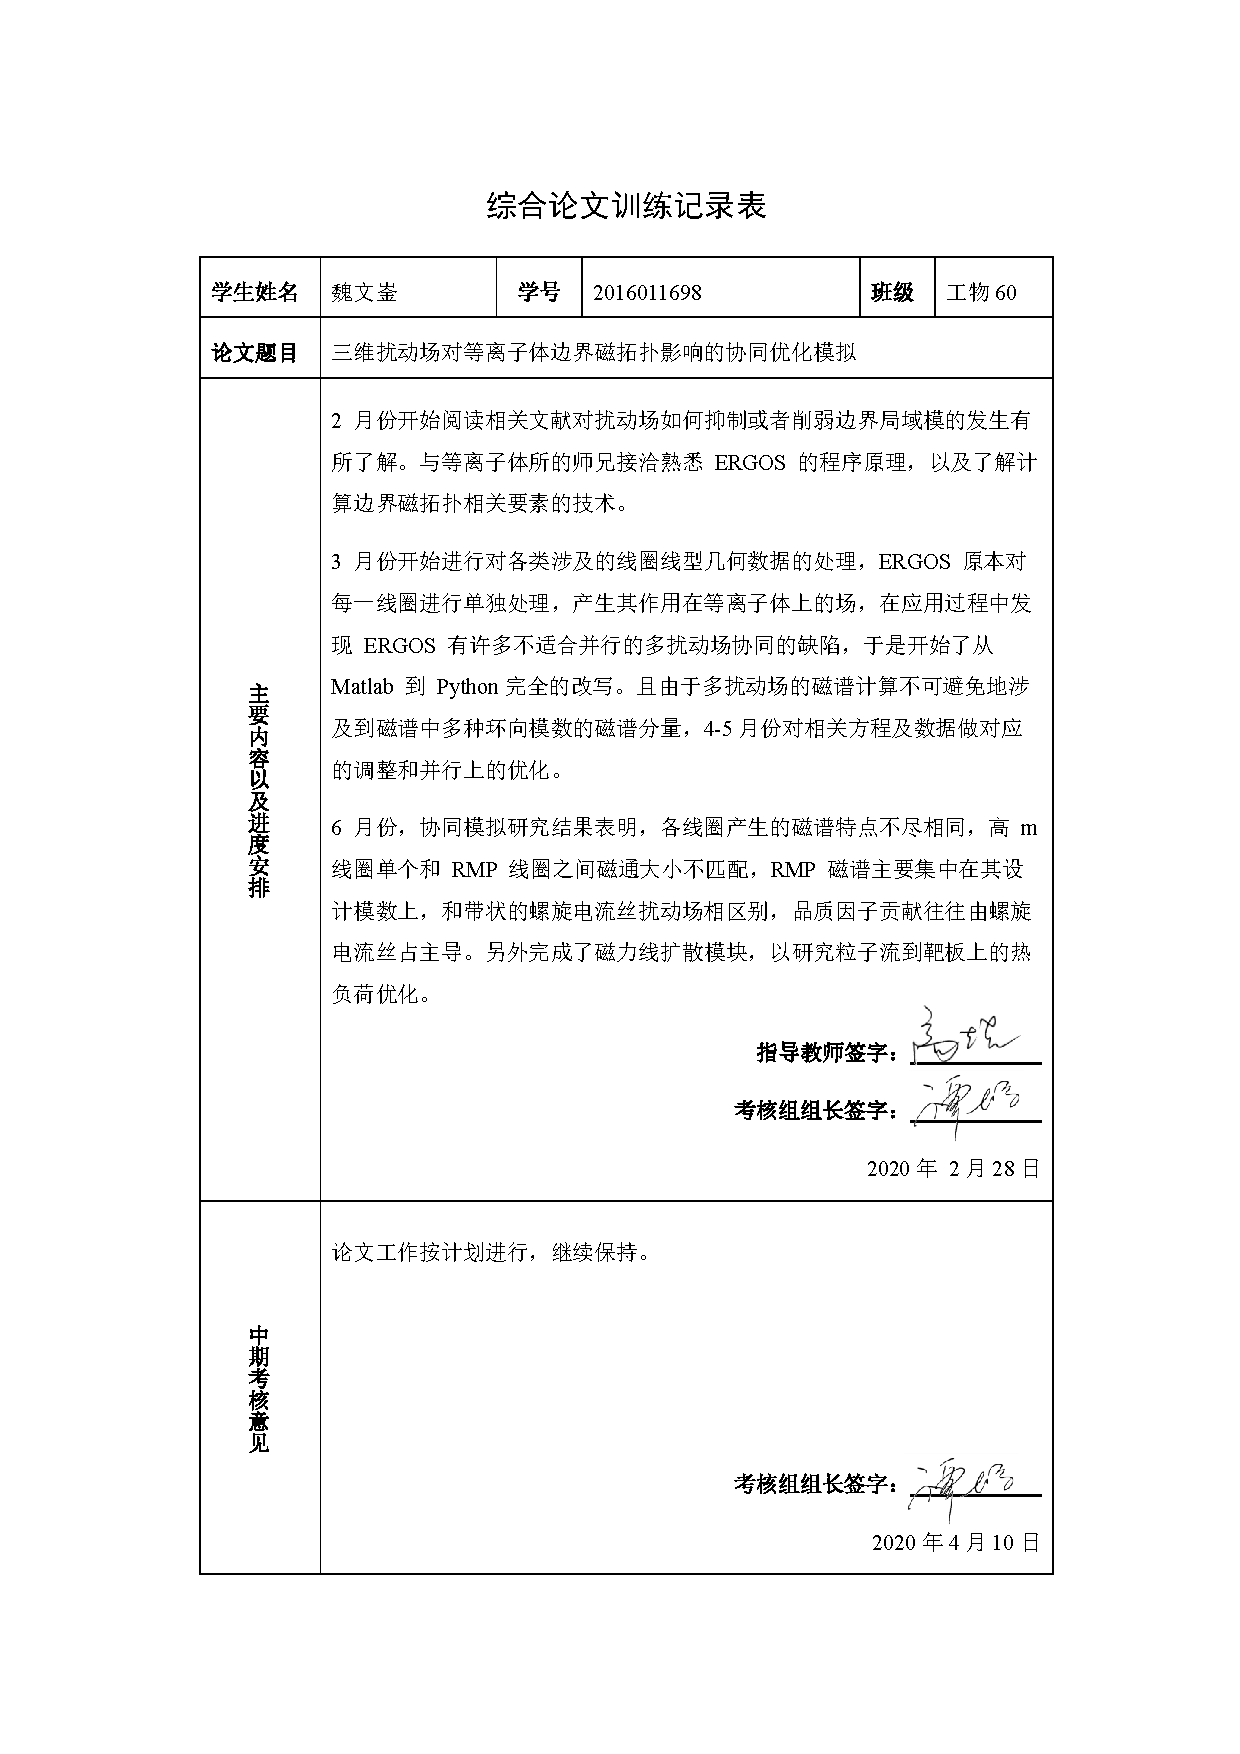
\includepdf[pages=-]{scan-record.pdf}
\end{document}
